\documentclass{book}
\usepackage{physics}
\usepackage{graphicx}
\usepackage{caption}
\usepackage{amsmath}
\usepackage{bm}
\usepackage{authblk}
\usepackage{amsfonts}
\usepackage{esint}
\usepackage{centernot}
\usepackage{mathtools}
\usepackage{amsthm}
\theoremstyle{definition}
\newtheorem{defn}{Definition}[section]
\newtheorem{prop}{Proposition}[section]
\newtheorem{rmk}{Remark}[section]
\newtheorem{thm}{Theorem}[section]
\newtheorem{exmp}{Example}[section]
\newtheorem{prob}{Problem}[section]
\newtheorem{sln}{Solution}[section]
\newtheorem*{prob*}{Problem}
\newtheorem{exer}{Exercise}[section]
\newtheorem*{exer*}{Exercise}
\newtheorem*{sln*}{Solution}
\usepackage{empheq}
\usepackage{hyperref}
\usepackage{tensor}
\usepackage{xcolor}
\hypersetup{
	colorlinks,
	linkcolor={black!50!black},
	citecolor={blue!50!black},
	urlcolor={blue!80!black}
}
\newcommand{\p}{\partial}
\newcommand{\R}{\mathbb{R}}
\newcommand{\C}{\mathbb{C}}
\newcommand{\lag}{\mathcal{L}}

\newcommand{\ham}{\mathcal{H}}

\newcommand{\I}{\mathcal{I}}
\newcommand{\K}{\mathcal{K}}
\newcommand{\F}{\mathcal{F}}
\newcommand{\w}{\omega}
\newcommand{\lam}{\lambda}
\newcommand{\al}{\alpha}
\newcommand{\be}{\beta}
\newcommand{\x}{\xi}

\newcommand{\f}[2]{\frac{#1}{#2}}

\newcommand{\ift}{\infty}

\newcommand{\lp}{\left(}
\newcommand{\rp}{\right)}

\newcommand{\lb}{\left[}
\newcommand{\rb}{\right]}

\newcommand{\lc}{\left\{}
\newcommand{\rc}{\right\}}


\newcommand{\V}{\mathbf{V}}
\newcommand{\U}{\mathcal{U}}
\newcommand{\Id}{\mathcal{I}}


%\setcounter{chapter}{-1}


\makeatletter
\renewcommand{\@chapapp}{Part}
%\renewcommand\thechapter{$\bf{\ket{\arabic{chapter}}}$}
%\renewcommand\thesection{$\bf{\ket{\arabic{section}}}$}
%\renewcommand\thesubsection{$\bf{\ket{\arabic{subsection}}}$}
%\renewcommand\thesubsubsection{$\bf{\ket{\arabic{subsubsection}}}$}
\makeatother



\usepackage{subfig}
\usepackage{listings}
\captionsetup[lstlisting]{margin=0cm,format=hang,font=small,format=plain,labelfont={bf,up},textfont={it}}
\renewcommand*{\lstlistingname}{Code \textcolor{violet}{\textsl{Mathematica}}}
\definecolor{gris245}{RGB}{245,245,245}
\definecolor{olive}{RGB}{50,140,50}
\definecolor{brun}{RGB}{175,100,80}
\lstset{
	tabsize=4,
	frame=single,
	language=mathematica,
	basicstyle=\scriptsize\ttfamily,
	keywordstyle=\color{black},
	backgroundcolor=\color{gris245},
	commentstyle=\color{gray},
	showstringspaces=false,
	emph={
		r1,
		r2,
		epsilon,epsilon_,
		Newton,Newton_
	},emphstyle={\color{olive}},
	emph={[2]
		L,
		CouleurCourbe,
		PotentielEffectif,
		IdCourbe,
		Courbe
	},emphstyle={[2]\color{blue}},
	emph={[3]r,r_,n,n_},emphstyle={[3]\color{magenta}}
}


\begin{document}
\begin{titlepage}\centering
 \clearpage
 \title{{\textsc{\textbf{QUANTUM\\ Mechanics, Optics, and Information}}}\\ \smallskip - A Quick Guide - \\}
 \author{\bigskip Huan Q. Bui}
  \affil{Colby College\\$\,$\\ PHYSICS \& MATHEMATICS\\ Statistics \\$\,$\\Class of 2021\\}
 \date{\today}
 \maketitle
 \thispagestyle{empty}
\end{titlepage}

\subsection*{Preface}
\addcontentsline{toc}{subsection}{Preface}

Greetings,\\

This text is my reading notes from Shankar's \textit{Principles of Quantum Mechanics, Second Edition}, \textit{Introductory Quantum Optics} by , \textit{Optical Coherence \& Quantum Optics}. Additional comes from my class notes, my comments/interpretations/solutions, and other books/articles/notes. There are three parts to this text, as the title suggests. The Quantum Mechanics part covers the principles of quantum mechanics. A majority of this part will be my reading notes from Shankar's book. The other two topics parts cover selected phenomena in quantum optics and quantum information theory.  \\

Background in linear algebra and modern physics (two semesters recommended) will be very helpful. I will try to cover some of the mathematical background, but a lot of familiarity will be assumed. \\

Enjoy!

\newpage
\tableofcontents
\newpage





\chapter{QUANTUM MECHANICS}


\newpage


\section{Mathematical Introduction}

\subsection{Linear Vector Spaces}

We should familiar with defining characteristics of linear vector spaces at this point. Here are some important definitions/theorems again:

\begin{defn}
	A linear vector space $\textbf{V}$ is a collection of objects called \textit{vectors} for which there exists
	
	\begin{enumerate}
		\item A definite rule for summing, and
		\item A definite rule for scaling, with the following features:
		
		
		\begin{itemize}
			\item Closed under addition: for $x,y \in \V$, $x+y \in \V$.
			\item Closed under scalar multiplication: $x\in \V$, then $ax \in \V$ for some scalar $a$.
			\item Scalar multiplication is distributive. 
			\item Scalar multiplication is associative.
			\item Addition is commutative.
			\item Addition is associative.
			\item There exists a (unique) null element in $\V$.
			\item There exists a (unique) additive inverse. 
		\end{itemize}
	\end{enumerate}
\end{defn}


Vector spaces are defined over some field. The field can be real numbers, complex numbers, or it can also be finite. As for good practice, we will begin to label vectors with Dirac bra-ket notation. So, for instance, $\ket{v} \in \V$ denotes vector $v \in \V$. Basic manipulations of these vectors are intuitive:
\begin{enumerate}
	\item $\ket{0}$ is unique, and is the null element.
	\item $0\ket{V} = \ket{0}$.
	\item $\ket{-V} = -\ket{V}$.
	\item $\ket{-V}$ is a unique additive inverse of $\ket{V}$.
\end{enumerate} 

The reasons for choosing to use the Dirac notation will become clear later on. Another important basic concept is \textit{linear (in)dependence}. Of course, there are a number of equivalent statement for linear independence. We shall just give one here:

\begin{defn}
	A set of vectors is said to be linearly independent if the only linear relation 
	\begin{align}
	\sum^n_{i=1}a_i\ket{i} = \ket{0}
	\end{align}
	is the trivial one where the components $a_i = 0$ for any $i$. 
\end{defn}



The next two basic concepts are \textit{dimension} and \textit{basis}. 

\begin{defn}
	A vector space $\V$ has dimension $n$ if it can accommodate a maximum of $n$ linearly independent vectors. We denote this $n$-dimensional vector space as $\V^n$.
\end{defn}

We can show that 

\begin{thm}
	Any vector $\ket{v} \in \V^n$ can be written (uniquely) as a linear combination of any $n$ linearly independent vectors.  
\end{thm}


\begin{defn}
	A set of $n$ linearly independent vectors in a $n$-dimensional space is called a \textit{basis}. So if $\ket{1},\dots,\ket{n}$ form a basis for $\V^n$, then any $\ket{v}\in \V$ can be written uniquely as
	\begin{align}
	\ket{v} = \sum^n_{i=1}a_i\ket{i}.
	\end{align}
\end{defn}

It is nice to remember the following:
\begin{align}
\boxed{\text{Linear Independence} = \text{Basis} + \text{Span}}
\end{align}

When a collection of vectors span a vector space $\V$, it just means that any $\ket{v} \in \V$ can be written as a linear combination of (some of) these vectors. 


The algebra of linear combinations is quite intuitive. If $\ket{v} = \sum_i a_i\ket{i}$ and $\ket{w} = \sum_i b_i\ket{i}$ then 

\begin{enumerate}
	\item $\ket{v + w} = \sum_i (a_i + b_i)\ket{i}$.
	\item $c\ket{v} = c\sum_i a_i\ket{i} = \sum_i ca_i\ket{i}$.
\end{enumerate}



A linear algebra text will of course provide a much better coverage of these topics. 















\subsection{Inner Product Spaces}


A generalization of the familiar dot product is the \textit{inner product} or the \textit{scalar product}. An inner product between two vectors $\ket{v}$ and $\ket{w}$ is denoted $\braket{v|w}$. An inner product has to satisfy the following properties:

\begin{enumerate}
	\item Conjugate symmetry (or skew-symmetry):$\braket{v}{w} = \braket{w}{v}^*$.
	\item Positive semi-definiteness: $\braket{v}{v} \geq 0$.
	\item Linearity in ket: $\braket{v}{aw + bz} = a\braket{v}{w} + b\braket{v}{z}$.
	\item Conjugate-linearity in bra: $\braket{av + bz}{w} = \bar{a}\braket{v}{w} + \bar{b}\braket{z}{w}$.
\end{enumerate}




\begin{defn}
	An inner product space is a vector space with an inner product. 
\end{defn}


\begin{defn}
	$\innerproduct{v}{w} = 0 \iff \ket{v} \perp \ket{w}$. 
\end{defn}


\begin{defn}
	The \textit{norm} (or length) of $\ket{v}$ is defined as 
	\begin{align}
	\norm{v} = \sqrt{\braket{v}}.
	\end{align}
	Unit vectors have unit norm. Unit vectors are said to be \textit{normalized}.  
\end{defn}




\begin{defn}
	A set of basis vectors all of unit norm, which are pairwise orthogonal will be called an \textit{orthonormal basis} or ONB. 
\end{defn}


Let $\ket{v} = \sum_i a_i\ket{i}$ and $\ket{w} = \sum_i b_i \ket{j}$, then 
\begin{align}
\braket{v}{w} = \sum_i a_i^*b_i \braket{i}{j}.
\end{align}



\begin{thm}
	\textbf{Gram-Schmidt:} Given a linearly independent basis, we can form linear combinations of the basis vectors to obtain an orthonormal basis. 
\end{thm}

Suppose that the Gram-Schmidt process gives us an ONB then we have
\begin{align}
\braket{i}{j} = \delta_{ij}.
\end{align}
As a result,
\begin{align}
\braket{v}{w} = \sum_i v_i^*w_i.
\end{align}
Alternatively, we can think this as doing the standard inner products of vectors whose entries are the components of the vectors $\ket{v}$, $\ket{w}$ in the basis:
\begin{align}
\ket{v} \to \begin{bmatrix}
v_1\\v_2\\\vdots\\v_n
\end{bmatrix}\hspace{0.5cm}
\ket{w} \to \begin{bmatrix}
w_1\\w_2\\\vdots\\w_n
\end{bmatrix} \implies \braket{v}{w} = \begin{bmatrix}
v_1^* & v_2^* & \dots & v_n^*
\end{bmatrix}\begin{bmatrix}
w_1\\ w_2 \\\vdots \\ w_n
\end{bmatrix}.
\end{align}
We can also easily see that 
\begin{align}
\braket{v}{v} = \sum_i \abs{v_i}^2 \geq 0.
\end{align}

\subsection{Dual Spaces and Dirac Notation}
Here we deal with some technical details involving the \textit{ket} (the column vectors) and the \textit{bra} (the row vectors). Column vectors are concrete manifestations of an abstract vector $\ket{v}$ in a basis, and we can work backward to go from the column vectors to the kets. We can do a similar thing with the bra vectors - since there's nothing special about writing the entries is a column versus in a row. However, we will do the following. We know that associated with every ket $\ket{v}$ is a column vector. So let its adjoint, which is a row vector, be associated with the bra, called $\bra{v}$. Now, we have two vector spaces, the space of kets and the dual space of bras. There is a basis of vectors $\ket{i}$ for expanding kets and a similar basis $\bra{i}$ for expanding bras. 

\subsubsection{Expansion of Vectors in an ONB}
It is extremely useful for us to be able to express a vector in an ONB. Suppose we have a vector $\ket{v}$ in an ONB $\ket{i}$. Then, let $\ket{v}$ be written as
\begin{align}
\ket{v} = \sum_i v_i \ket{i}.
\end{align}
To find the components $v_i$, we take the inner product of $\ket{v}$ with $\ket{j}$:
\begin{align}
\braket{j}{v} = \sum_i v_i \braket{j}{i} = \sum_i v_i\delta_{ij} = v_j.
\end{align}
With this, we can rewrite the vector $\ket{v}$ in the basis $\ket{i}$ as
\begin{align}
\ket{v} = \sum_i \ket{i}\braket{i}{v}.
\end{align}



\subsubsection{Adjoint Operations}
Here is a few details regarding taking the adjoints of vectors. Suppose that
\begin{align}
\ket{v} = \sum_i v_i\ket{i} = \sum_i \ket{i}\braket{i}{v}.
\end{align}
Then,
\begin{align}
\bra{v} = \sum_i\ket{i}v_i^*.
\end{align}
Now, because $v_i = \braket{i}{v}$, we have $v_i^* = \braket{v}{i}$. Thus, 
\begin{align}
\bra{v} = \sum_i \braket{v}{i}\bra{i}.
\end{align}
In plain words, the rule for taking the adjoint is the following. To take the adjoint of an equation involving bras and kets and coefficients, reverse the order of all factors, exchanging bras and kets and complex conjugating all coefficients. 


\subsubsection{Gram-Schmidt process}
Again, the Gram-Schmidt process lets us convert a linearly independent basis into an orthonormal one. For a two-dimensional case, procedure is the following:
\begin{enumerate}
	\item Rescale the first by its own length, so it becomes a unit vector. This is the first (orthonormal) unit vector.
	\item Subtract from the second vector its projection along the first, leaving behind only the part perpendicular to the first. (Such a part will remain since by assumption the vectors are nonparallel).
	\item Rescale the left over piece by its own length. We now have the second basis vector: it s orthogonal to the first and of unit length.
\end{enumerate}

In general, let $\ket{I}, \ket{II}, \dots$ be a linearly independent basis. The first vector of the orthonormal basis will be
\begin{align}
\ket{1} = \f{\ket{I}}{\norm{\ket{I}}}.
\end{align}
For the second vector in the basis, consider
\begin{align}
\ket{2'} = \ket{II} - \ket{1}\braket{1}{II}.
\end{align}
We can see that $\ket{2'}$ is orthogonal to $\ket{1}$:
\begin{align}
\braket{1}{2'} = \braket{1}{II} - \braket{1}\braket{1}{II} = 0.
\end{align}
So dividing $\ket{2'}$ by its norm gives us, $\ket{2}$, the second element in the ONB. To find the third element in the ONB, we have to first make sure it is orthogonal to both $\ket{I}$ and $\ket{II}$, so let us consider
\begin{align}
\ket{3'}= \ket{III} - \ket{1}\braket{1}{III} - \ket{2}\braket{2}{III}.
\end{align}
Once again we have $\ket{3'}$ orthogonal to both $\ket{1}$ and $\ket{2}$. Normalizing $\ket{3'}$ gives us $\ket{3}$, the third element in the ONB. We can now see how this process continues to the last element. 



\subsubsection{Schwarz and Triangle Inequality}
Just two small yet very important details:
\begin{thm}
	Schwarz Inequality:
	\begin{align}
	\abs{\braket{v}{w}} \leq \norm{v}\norm{w}
	\end{align}
\end{thm}


\begin{thm}
	Triangle Inequality:
	\begin{align}
	\norm{v+w} \leq \norm{v} + \norm{w}.
	\end{align}
\end{thm}



\subsection{Subspaces, Sum and Direct Sum of Subspaces}
I'm not too happy with the definitions given by Shankar's book. He also uses the notation for direct sum to indicate vector space addition, which is very confusing. Any linear algebra textbook would provide better definitions. For equivalent statements about directness of vector space sums, check out my \href{https://huanqbui.com/LaTeX\%20projects/Matrix_Analysis/HuanBui_MatrixAnalysis.pdf}{Matrix Analysis} notes. 




\subsection{Linear Operators}
Again, a rigorous definition of an operator can be found in almost any linear algebra textbook. But here,we can simply think of an operator as just some linear transformation from a vector space to itself. Say, if $\Omega$ is some operator that sends $\ket{v}$ to $\ket{v'}$, we write
\begin{align}
\Omega\ket{v} = \ket{v'}.
\end{align}
By definition, $\ket{v}$ and $\ket{v'}$ are contained in the same vector space. Now, we note that $\Omega$ can also act on bras:
\begin{align}
\bra{v}\Omega = \bra{v'}.
\end{align}
But of course the order of writing things is different, and once again, $\bra{v}$ and $\bra{v'}$ are contained in the same (dual) space. 


Next, because $\Omega$ is linear, we have the following familiar rules:
\begin{align}
\Omega \alpha \ket{v_i} &= \alpha\Omega \ket{v_i}.\\
\Omega \{ \alpha \ket{v_i} + \beta\ket{v_j} \} &= \alpha\Omega\ket{v_i} + \beta\Omega \ket{v_j}.\\
\bra{v_i}\alpha\Omega &= \bra{v_i}\Omega \alpha\\
\{\bra{v_i}\alpha + \bra{v_j}\beta \}\Omega &= \alpha\bra{v_i}\Omega + \beta \bra{v_j}\Omega.
\end{align}


One of the nice features of linear operators is that the action of an operator is completely determined by what it does to the basis vectors. Suppose 
\begin{align}
\ket{v} = \sum_i v_i \ket{i}
\end{align}
and 
\begin{align}
\Omega\ket{i} = \ket{i'},
\end{align}
then
\begin{align}
\Omega \ket{v} = \sum_i \Omega v_i \ket{i}= \sum_iv_i \Omega\ket{i} = \sum_iv_i\ket{i'}.
\end{align}



The next point of interest is \textit{products} of operators. As we might have seen, operators don't always commute. A product of operators applied to a vector just means operators are applied in sequence. The \textit{commutator} of two operators $\Omega, \Lambda$ is defined as
\begin{align}
\Omega\Lambda - \Lambda\Omega \equiv \lb \Omega,\Lambda \rb.
\end{align}
In general, $\lb \Omega,\Lambda\rb$ is not zero. Suppose three operators $\Omega, \Lambda, \Theta$ are involved, then we have two useful relations:
\begin{align}
&\lb \Omega, \Lambda\Theta \rb = \Lambda\lb \Omega, \Theta \rb + \lb \Omega, \Lambda \rb \Theta\\
&\lb \Lambda\Omega, \Theta \rb = \Lambda\lb \Omega, \Theta \rb + \lb \Lambda, \Theta \rb \Omega.
\end{align}
We notice that the form resembles the chain rule in calculus. 





\subsection{Matrix Elements of Linear Operators}
One thing we will hear very often in quantum mechanics is the idea of matrix elements. The idea, it turns out, is very simple. Suppose we have a basis $\ket{i}$, and an operator $\Omega$ such that
\begin{align}
\Omega\ket{i} = \ket{i'}.
\end{align}
Then, for
\begin{align}
\ket{v} = \sum_i v_i \ket{i}, 
\end{align}
we have
\begin{align}
\Omega\ket{v} = \Omega \sum_i v_i \ket{i} = \sum_i v_i \Omega\ket{i} = \sum_i v_i \ket{i'}.
\end{align}
Because we know $\Omega$ and $\ket{i}$, $\ket{i'}$ is also known, as in its components in the basis $\ket{j}$ (un-primed) are known:
\begin{align}
\braket{j}{i'} = \bra{j}\Omega\ket{i} \equiv \Omega_{ji},
\end{align}
where the $n^2$ numbers $\Omega_{ji}$ are the matrix elements of $\Omega$ in this basis. Now, if
\begin{align}
\Omega\ket{v} = \ket{v'}
\end{align}
then the components of the transformed ket $\ket{v'}$ can be expressed in terms of the components of $\ket{v}$ and the matrix elements $\Omega_{ji}$:
\begin{align}
v_i' = \braket{i}{v'} = \bra{i}\Omega\ket{v} = \bra{i}\Omega \sum_j v_j \ket{j} = \sum_j v_j \bra{i}\Omega\ket{j} = \sum_j \Omega_{ij}v_j.
\end{align}
We can see the above equation in matrix form as well:
\begin{align}
\begin{bmatrix}
v_1'  \\ \vdots \\ v_n'
\end{bmatrix}
=
\begin{bmatrix}
\bra{1}\Omega\ket{1} &  \dots & \bra{1}\Omega\ket{n} \\
\vdots & \ddots & \vdots\\	
\bra{n}\Omega\ket{1} & \dots & \bra{n}\Omega\ket{n} \\
\end{bmatrix}
\begin{bmatrix}
v_1 \\ \vdots \\ v_n 
\end{bmatrix}.
\end{align}
The elements of the first column are simply the components of the first transformed basis vector $\ket{1'} = \Omega\ket{1}$ in the given basis. Likewise, the elements of the j$^{\text{th}}$ column represent the image of the j$^\text{th}$ basis vector after $\Omega$ acts on it. 


\subsection{Matrix Elements of Products of Operators}

To get the matrix elements of a product of two operators, we do the following. Suppose we have operators $\Omega$ and $\Lambda$, then
\begin{align}
(\Omega\Lambda)_{ij} = \bra{i}\Omega\Lambda\ket{j} = \bra{i}\Omega \mathcal{I} \Lambda \ket{j}.
\end{align}
Now, we observe that 
\begin{align}
\mathcal{I} = \sum_k \ket{k}\bra{k}. 
\end{align}
So, 
\begin{align}
(\Omega \Lambda)_{ij} = \sum_k \bra{i}\Omega\ket{k}\bra{k}\Lambda \ket{j} = \sum_k \Omega_{ik}\Lambda_{kj}.
\end{align}



\subsection{The Adjoint of an Operator}
Recall that for a scalar $\alpha$
\begin{align}
\bra{\alpha v} = \bra{v}\alpha^*,
\end{align}
then we have a similar thing with operators if
\begin{align}
\Omega\ket{v} = \ket{v'}
\end{align}
then 
\begin{align}
\bra{\Omega v} = \bra{v}\Omega^\dagger,
\end{align}
where $\Omega^\dagger$ is \textit{the} adjoint of $\Omega$. The relationship between $\Omega^\dagger$ and $\Omega$ can be seen in a basis. We consider the matrix elements of $\Omega^\dagger$ in a basis:
\begin{align}
(\Omega^\dagger)_{ij} = \bra{i}\Omega^\dagger \ket{j} = \bra{\Omega i}\ket{j} = \bra{j}\ket{\Omega i}^* = \bra{j} \Omega \ket{i}^* = \Omega_{ji}^*.
\end{align}
We see that
\begin{align}
\Omega^\dagger_{ij} = \Omega^*_{ji},
\end{align}
i.e., in matrix form, $\Omega^\dagger$ is the conjugate transpose of $\Omega$. 

The rule for taking adjoins of equations is rather simple: When a product of operators, bras, kets, ad explicit numerical coefficients is encountered, reverse the order of all factors and make the substitution $\Omega \leftrightarrow \Omega^\dagger$, $\ket{} \leftrightarrow \bra{}$, $a \leftrightarrow a^*$. 


\subsection{Hermitian, Anti-Hermitian, and Unitary Operators}

\begin{defn}
	An operator $\Omega$ is Hermitian $\iff \Omega = \Omega^\dagger$.
\end{defn}


\begin{defn}
	An operator $\Omega$ is anti-Hermitian $\iff \Omega = -\Omega^\dagger$.
\end{defn}

Shankar's book ignores a bigger class of operators called \textit{normal} operators. Normal operators commute with their adjoints. In a sense, normal operators act \textit{like numbers}. Hermitian (or self-adjoint) operators are a subset of normal operators. So, the number-likeness of normal operators carries over to Hermitian operators and anti-Hermitian operators as well. Hermitian and anti-Hermitian operators are like pure real and pure imaginary numbers. Just as every number maybe be decomposed into a sum of pure real and pure imaginary parts, it turns out that we can decompose every operator into its Hermitian and anti-Hermitian parts. 
\begin{align}
\Omega = \f{\Omega + \Omega^\dagger}{2} + \f{\Omega - \Omega^\dagger}{2}.
\end{align}
One can verify that the first terms is Hermitian, and the second term is anti-Hermitian. 




\begin{defn}
	An operator $\mathcal{U}$ is unitary $\iff \mathcal{U}\mathcal{U}^\dagger = \mathcal{I}$. 
\end{defn}

Unitary operators are like complex numbers of unit modulus. 


\begin{thm}
	Unitary operators preserves the inner product between the vectors they act on.
	\begin{proof}
		Suppose
		\begin{align}
		\ket{v'} &= \mathcal{U}\ket{v}\\
		\ket{w'} &= \mathcal{U}\ket{w}.
		\end{align}
		Then
		\begin{align}
		\braket{v'}{w'} = \braket{\mathcal{U}v}{\mathcal{U}w} = \bra{v}\mathcal{U}^\dagger\mathcal{U}\ket{w} = \braket{v}{w}.
		\end{align}
	\end{proof}
\end{thm} 



\begin{thm}
	The columns (or rows) of a unitary matrix form an ONB.
	\begin{proof}
		Refer to a linear algebra text. The key is to consider an inner product between any two columns/rows.
	\end{proof}
\end{thm}


\subsection{Active and Passive Transformation}

Suppose all $\ket{v}$ is unitarily transformed to $\ket{v'}$:
\begin{align}
\ket{v} \to \U \ket{v}.
\end{align}
Then under this transformation, the matrix elements of any operator $\Omega$ are modified as follows:
\begin{align}
\ket{v'}\Omega\ket{v} \to \ket{\U v'} \Omega \ket{\U v} = \bra{v'}\U^\dagger \Omega \U \ket{v}.
\end{align}
It is clear that the same change is equivalent to leaving the vectors alone and subjecting all operators to the change
\begin{align}
\Omega \to \U^\dagger \Omega \U.
\end{align}

\textit{Active transformation} refers to changing the vectors, while \textit{passive transformation} refers to changing the operators.





\subsection{The Eigenvalue Problem}
I won't say much about what eigenvectors and eigenvalues are because we should be familiar with these concepts at this point. But just to introduce some terminology, each operator has certain kets of its own called \textit{eigenkets}, on which its action is simply that of scaling. So, eigenkets are just a different word for eigenvectors of an operator:
\begin{align}
\Omega\ket{v} = \omega\ket{v}.
\end{align}

Shankar's book talks about the characteristic equation and characteristic polynomial. While these are legitimate ways to find eigenvalues and eigenvectors, it is often very difficult. I'd prefer Leo Livshits' and Sheldon Axler's way and use minimal polynomials instead. I would steer away from determinants and characteristic polynomials at this point. 


\begin{thm}
	Eigenvalues of a Hermitian operator are real. 
	\begin{proof}
		Suppose 
		\begin{align}
		\Omega\ket{w} = a\ket{w},
		\end{align}
		then
		\begin{align}
		\bra{w}\Omega\ket{w} = a\braket{w},
		\end{align}
		and thus
		\begin{align}
		a^* \braket{w} = \bra{w}\Omega^\dagger\ket{w} = \bra{w}\Omega\ket{w} = a\braket{w}.
		\end{align}
		So we have
		\begin{align}
		(a - a^*)\braket{w} = 0.
		\end{align}
		Because $\ket{w}$ are eigenkets, they are cannot be the zero vector. This means $a = a^*$.
	\end{proof}
\end{thm}


Some might worry about the existence of eigenvalues of Hermitian operators. But worry no more, because Hermitian operators are a subclass of normal operators, which are a subclass of diagonalizable operators. This simply says Hermitian matrices are diagonalizable, and all its eigenvalues are real. But it turns out there is a little bit more to this. 


\begin{thm}
	For every Hermitian operator $\Omega$, there exists an ONB comprised entirely of the eigenvectors of $\Omega$. 
\end{thm}

Once again, this should be no surprise if one has studied normal operators. Hermitian operators inherit this property from its normalness. This property of normal operators are called the Spectral Theorem (for normal operators, of course). The proof of all this can be found in many linear algebra texts. 


\begin{thm}
	The eigenvalues of a unitary operator are complex numbers of unit modulus. 
	\begin{proof}
		The key to the proof is using inner products. 
	\end{proof}
\end{thm}



\subsubsection{Simultaneous Diagonalization of Two Hermitian Operators}

I would say the topic of simultaneous diagonalizability is covered quite well in Leo Livshits' course and hence in my \href{https://huanqbui.com/LaTeX\%20projects/Matrix_Analysis/HuanBui_MatrixAnalysis.pdf}{Matrix Analysis} notes. But here I will just give the most important results. 

\begin{thm}
	If $\Omega$ and $\Lambda$ are two commuting Hermitian operators, there exists a basis of common eigenvectors that diagonalizes them both. 
\end{thm} 

This result is not too surprising if we have studied simultaneous diagonalizability before. A more general theorem says that 
\begin{align}
\text{Simultaneous diagonalizbility} \iff \text{Individual diagonalizability} + \text{Commutativity}.
\end{align}
It is clear that because all Hermitian operators are diagonalizable, if two Hermitian operators commute, they are simultaneously diagonalizable.



\subsubsection{The Propagator}

In quantum mechanics (and classical mechanics of course), it is quite common to have some final state vector be obtained from an initial state vector multiplied by some matrix, which is independent of the initial state. We call this matrix the \textit{propagator}. 


The central problem in quantum mechanics is finding the state of a quantum system $\ket{\psi}$, which obeys the Schr\"{o}dinger equation:
\begin{align}
i\hbar \ket{\dot{\psi}} = J\ket{\psi}
\end{align}
where the Hermitian operator $H$ is called the \textit{Hamiltonian}. We will see much more of this as we move on.



\subsection{Functions of Operators and Related Concepts}


In this section, we look at whether it makes sense to define functions of operators. We will only restrict ourselves to functions that can be written as a power series. Consider a series
\begin{align}
f(x) = \sum_{n=0}^\infty = a_n x^n
\end{align}
where $x$ is a scalar. We defined the same function of an operator to be
\begin{align}
f(\Omega) = \sum_{n=0}^\infty a_n\Omega^n.
\end{align}
Now, this definition only makes sense if we have convergence. Consider this example:
\begin{align}
e^\Omega = \sum^\infty_{n=0}\f{\Omega^n}{n!},
\end{align}
where $\Omega$ is Hermitian. In the eigenbasis of $\Omega$, $\Omega$ is diagonal. This means we can add and/or take powers of $\Omega$ by add and/or take powers of the diagonal entries. We can find that
\begin{align}
e^\Omega = \begin{bmatrix}
\sum^\infty_{m=0}\f{\omega^m_1}{m!}&&\\
&&\\
&&\sum^\infty_{m=0}\f{\omega^m_n}{m!}
\end{bmatrix}
\end{align}
where $\omega_i$ are the eigenvalues of $\Omega$. We note that each entry in the expression above converges to $e^{\omega_i}$.



\subsubsection{Derivatives of Operators with Respect to Parameters}
Now, consider some operator $\Theta(\lambda)$ that depends on a parameter $\lambda$. The derivative of $\Theta$ with respect to $\lambda$ is defined to be
\begin{align}
\f{d\Theta(\lambda)}{d\lambda} = \lim_{\Delta\lambda \to 0} \lb \f{\Theta(\lambda + \Delta \lambda) - \Theta(\lambda)}{\Delta \lambda} \rb.
\end{align}
If $\Theta(\lambda)$ is written as a matrix, then the matrix of $d\Theta/d\lambda$ is obtained by differentiating the matrix elements of $\Theta(\lambda)$. A case that might be interesting to us is 
\begin{align}
\Theta(\lambda) = e^{\lambda\Omega}.
\end{align}
It turns out that if $\Omega$ is Hermitian or ``nice enough'' then 
\begin{align}
\f{d\Theta(\lambda)}{d\lambda} = \Omega e^{\lambda\Omega} = e^{\lambda\Omega}\Omega = \Theta(\lambda)\Omega = \Omega \Theta(\lambda).
\end{align}
Conversely, if we have
\begin{align}
\f{d\Theta(\lambda)}{d\lambda} = \Theta(\lambda)\Omega
\end{align}
then 
\begin{align}
\Theta(\lambda) = ce^{\lambda\Omega}
\end{align}
where $c$ is some operator. But we have to be careful that $c$ might not commute with $e^{\lambda\Omega}$.

The business of whether two operators commute or don't can make things slightly more complicated. If $\Theta$ and $\Omega$ commute, i.e., $[\Theta, \Omega] = 0$, then the rules of exponentiation carries over very nicely:
\begin{align}
&e^{a\Omega}e^{b\Omega} = e^{(a + b)\Omega}\\
&e^{a\Omega}e^{b\Theta} = e^{a\Omega + b\Theta}\\
&e^{a\Omega}e^{b\Theta}e^{-a\Omega} = e^{b\Theta}.
\end{align}
If $[\Omega, \Theta] \neq 0$, then the second and third equations no longer hold. Likewise, in differentiating a product, we have to be extra careful:
\begin{align}
\f{d}{d\lambda}e^{\lambda\Omega}e^{\lambda\Theta} = \Omega e^{\lambda\Omega}e^{\lambda\Theta} + e^{\lambda\Omega}e^{\lambda\Theta}\Theta.
\end{align}
While $[\Omega, e^{\lambda\Omega}] = 0$, because $\Theta$ and $\Omega$ might not commute, we can't bring $\Omega$ over to the right of $e^{\lambda\Theta}$. 


\subsection{Generalization to Infinite Dimensions}


\subsubsection{The Dirac delta function}
Consider the ordered $n$-tuple $\{ f_n(x_1), \dots, f_n(x_n) \}$ as components of a ket $\ket{f_n}$ in a vector space $\V^n(\mathbb{R})$:
\begin{align}
\ket{f_n} \leftrightarrow \begin{bmatrix}
f_n(x_1) \\ \vdots \\ f_n(x_n)
\end{bmatrix}.
\end{align}
The basis vectors in this space are:
\begin{align}
\ket{x_i} \leftrightarrow \begin{bmatrix}
0 \\ 0 \\ \vdots \\ 1 \\ 0 \\ \vdots \\ 0
\end{bmatrix} \leftarrow i^{th} \text{place}.
\end{align}
The basis vectors satisfy \textit{orthogonality} and \textit{completeness}:
\begin{align}
&\braket{x_i}{x_j} = \delta_{ij}\\
&\sum_{i=1}^n \ket{x_i}\bra{x_i} = \Id.
\end{align}
With this,
\begin{align}
\ket{f_n} = \sum_{i=1}^n f_n(x_i)\ket{x_i}.
\end{align}
We next define the inner product in this space:
\begin{align}
\braket{f_n}{g_n} \ sum^n_{i=1}f_n(x_i)g_n(x_i).
\end{align}
The functions $f_n$ and $g_n$ are said to be orthogonal if $\braket{f_n}{g_n} = 0$. We also have that
\begin{align}
\braket{f_n}{f_n} = \sum^n_{i=1}[f_n(x_i)]^2.
\end{align}
For finite $n$, nothing ``bad'' can really happen here. But what if $n$ is infinity? What we need is the redefinition of the inner product for finite $n$ in such a way that as $n$ goes to infinity, we get a smooth limit. A natural choice is
\begin{align}
\braket{f_n}{g_n} = \sum^n_{i=1} f_n(x_i)g_n(x_i)\f{L}{n+1}
\end{align}
where $L$ is the length of the interval. If we now let $n$ go to infinity, we get
\begin{align}
&\braket{f}{g} = \int^L_0 f(x)g(x)\,dx\\
&\braket{f} = \int^L_0 f^2(x)\,dx.
\end{align}
Now, if we consider complex functions as well in some interval $a\leq x \leq b$, the inner product becomes:
\begin{align}
\braket{f}{g} = \int^b_a f^*(x)g(x)\,dx.
\end{align}
But what are the basis vectors in this space and are they normalized? We know that 
\begin{align}
\braket{x}{x'} = 0
\end{align}
if $x \neq x'$. But what if $x = x'$? It turns out that we cannot simply require $\braket{x}{x} = 1$. The best way to see this is to deduce the correct normalization. We start with the completeness relation:
\begin{align}
\int^b_a \ket{x'}\bra{x'}\,dx' = \Id. 
\end{align}
Now, consider this
\begin{align}
\int^b_a \braket{x}{x'}\braket{x'}{f}\,dx' = \bra{x}\Id \ket{f} = \braket{x}{f}.
\end{align}
This is nothing but the projection of $\ket{f}$ along the basis ket $\ket{x}$, which is just $f(x)$. So, we also have $f(x') = \braket{x'}{f}$. Let the inner product $\braket{x}{x'}$ be some unknown function $\delta(x,x')$. Since $\delta(x,x')$ vanishes if $x\neq x'$, we can restrict the integral to an infinitesimal region near $x'=x$. With these, the equality above gives
\begin{align}\label{delt}
\int^{x+\epsilon}_{x-\epsilon}\delta(x,x')f(x')\,dx' = f(x).
\end{align}
In this infinitesimal region, $f(x)$ can assumed to be constant, and thus can be pulled out of the integral, leaving
\begin{align}
f(x)\int^{x+\epsilon}_{x-\epsilon} \delta(x,x')\,dx' = f(x).
\end{align}
And so we have
\begin{align}
\int^{x+\epsilon}_{x-\epsilon} \delta(x,x')\,dx' = 1. 
\end{align}
Clearly, $\delta(x,x')$ cannot be finite at $x=x'$. It should be infinite in such a way that its integral is 1. Since $\delta(x,x')$ depends only on the difference $x-x'$, we can write it as $\delta(x-x')$. So, the function $\delta(x-x')$ has the properties:
\begin{align}
\begin{cases}
\delta(x-x') = 0, \hspace{0.5cm} x \neq x'\\
\int^b_a \delta(x-x')\,dx' = 1\hspace{0.5cm} a < x < b
\end{cases}.
\end{align}
This is called the \textbf{Dirac delta function} and it fixes the normalization of the basis vectors:
\begin{align}
\braket{x}{x'} = \delta(x-x').
\end{align}

The Dirac delta function is ``strange'' in the sense that its value is either zero or infinite. It's thus useful to view it as the limit of a Gaussian:
\begin{figure}[!htb]
	\centering
	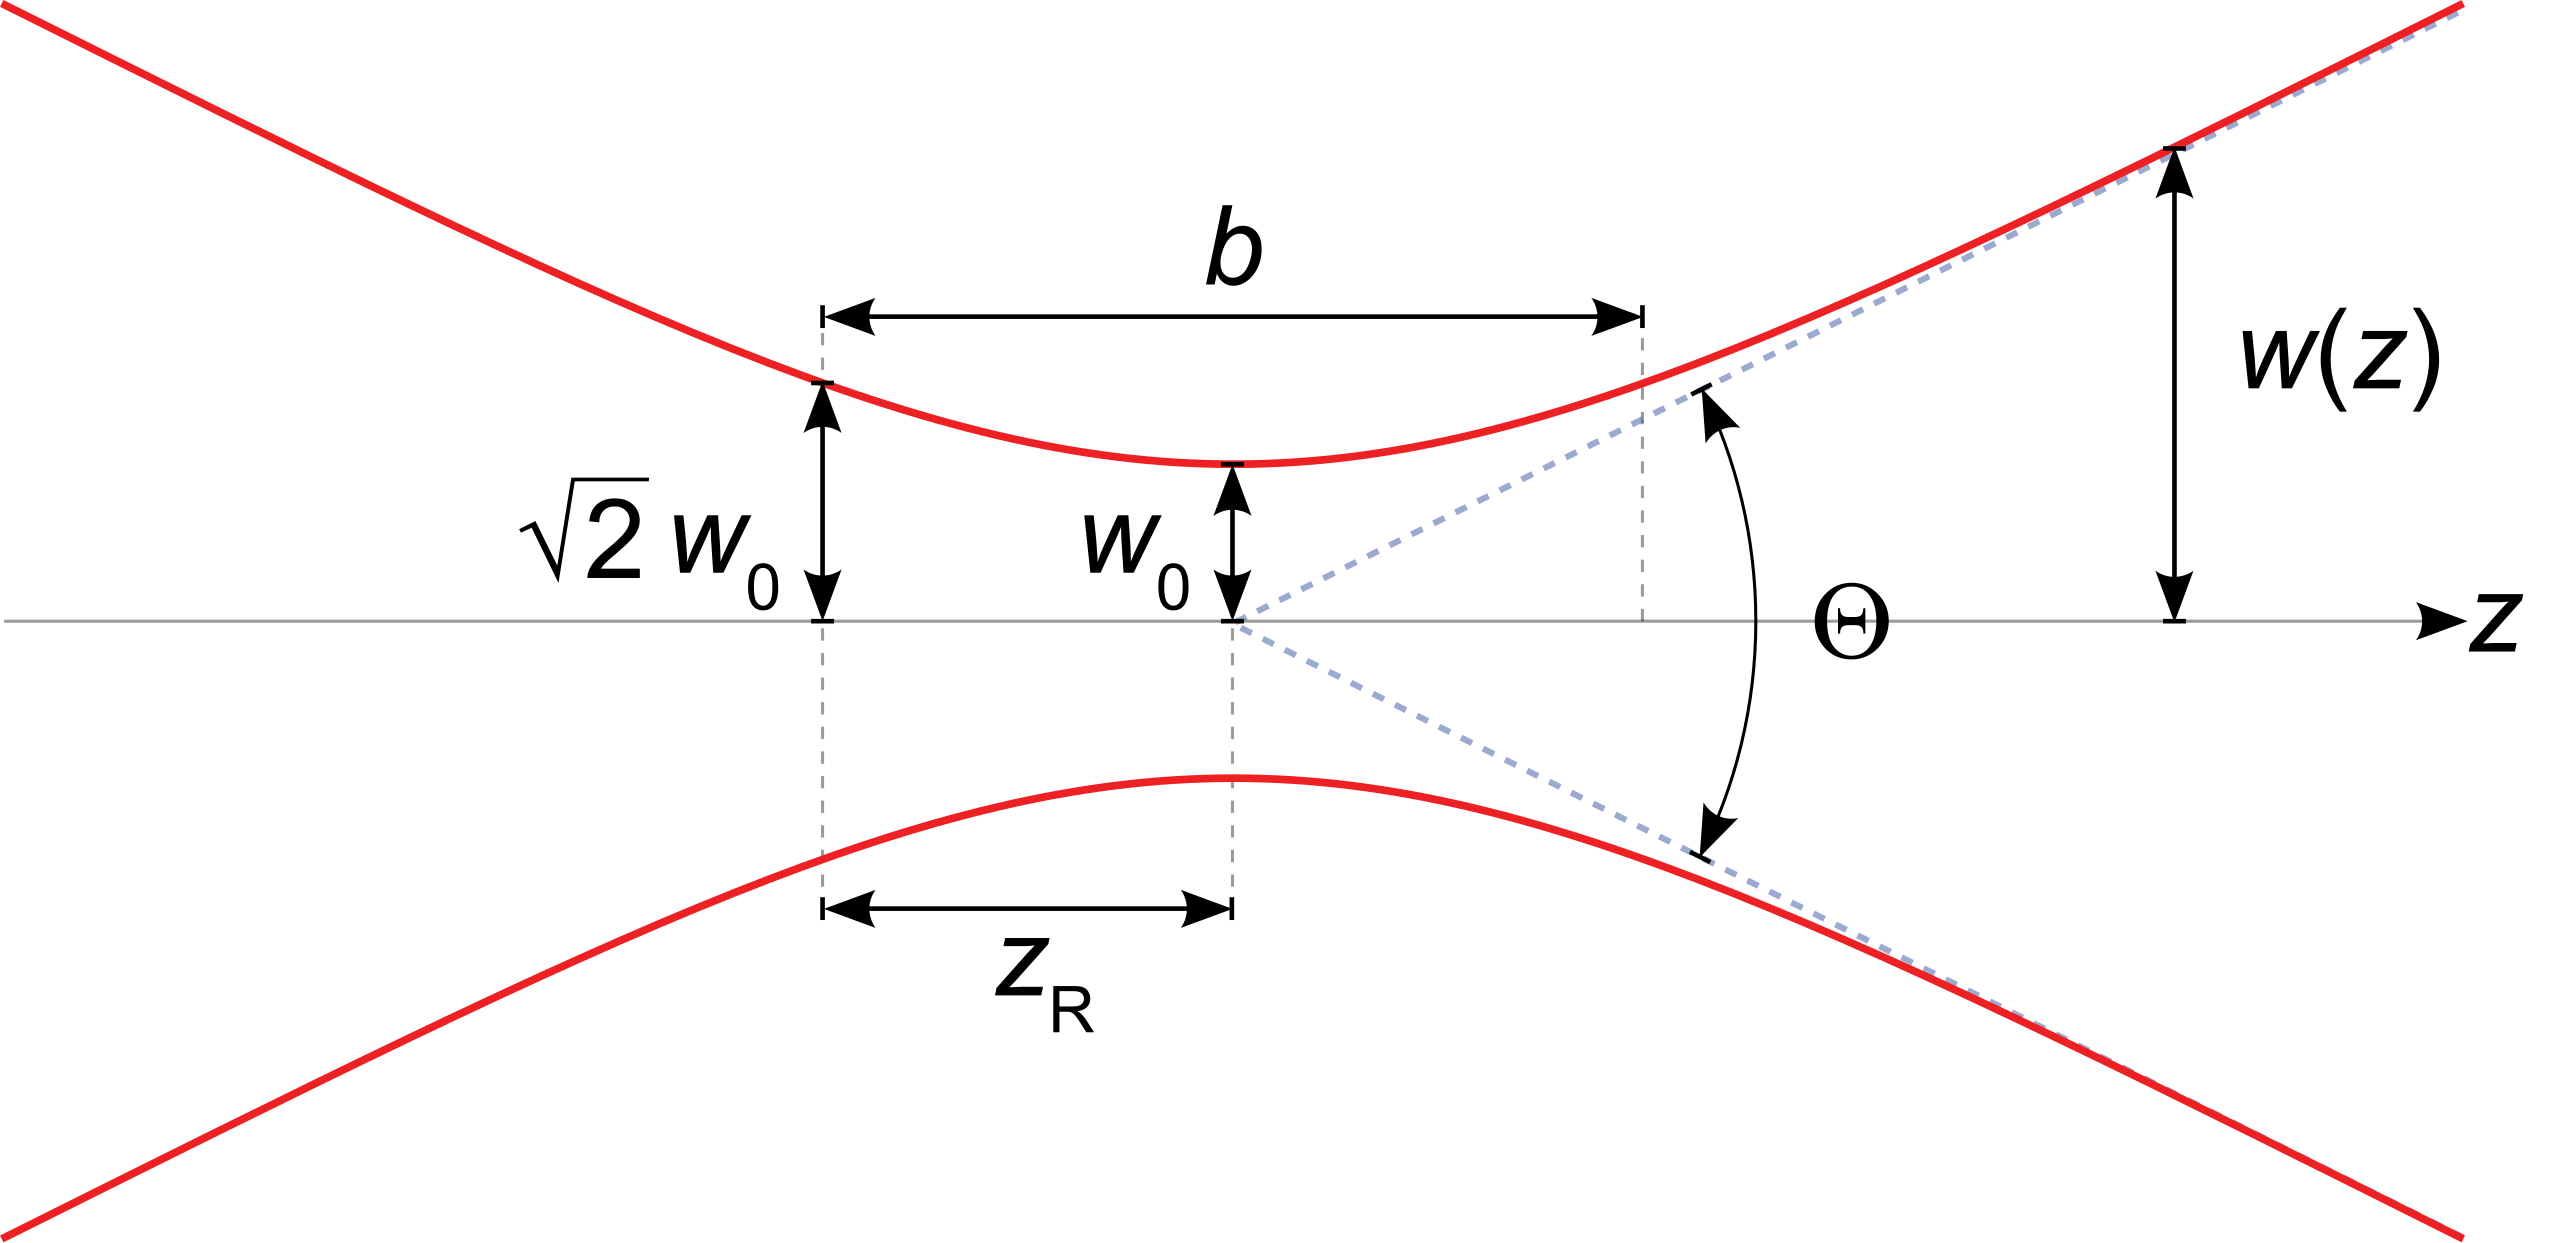
\includegraphics[scale=0.3]{gauss.png}
\end{figure}

of the form
\begin{align}
g_\Delta(x-x') = \f{1}{\sqrt{\pi \Delta^2}}e^{-(x-x')^2/\Delta^2}.
\end{align}
It is clear that the area under the curve is one (one can easily check this). Also, $\Delta \to 0$, $g_\Delta$ becomes closer and closer to $\delta(x-x')$ (the area under the curve is the same, while the width of the peak becomes smaller and smaller). 


From Gaussian model, we know that the delta function is not only real but also even:
\begin{align}
\delta(x-x') = \delta(x'-x).
\end{align}
Next, we consider the derivative of $\delta(x-x')$ with respect to $x$:
\begin{align}
\delta'(x-x') = \f{d}{dx}\delta(x-x') = -\f{d}{dx'}\delta(x-x').
\end{align}
Once again, we consider the Gaussian model. We consider $dg_\Delta(x-x')/dx = -dg_\Delta(x-x')/dx'$ as a function of $x'$:
\begin{figure}[!htb]
	\centering
	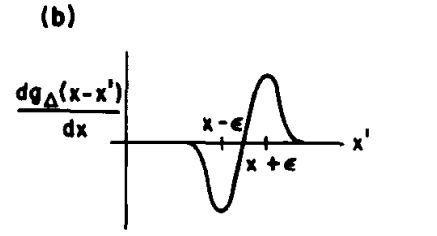
\includegraphics[scale=0.5]{dgauss.png}
\end{figure}

As $g_\Delta$ shrinks,, each bump at $\pm \epsilon$ will become, up to a scale factor, the $\delta$ function, such that
\begin{align*}
\int\delta'(x-x')f(x')\,dx' \propto   f(x+\epsilon) - f(x-\epsilon) = 2\epsilon\f{df}{dx'}\bigg\vert_{x=x'}.
\end{align*}
The constant of proportionality turns out to be $\epsilon/2$, and so
\begin{align}
\int \delta'(x-x')f(x')\,dx' = \f{df}{dx'}\bigg\vert_{x=x'} = \f{df(x)}{dx}.
\end{align}
In short, we can describe the $\delta'$ function as 
\begin{align}
\delta'(x-x') = \delta(x-x')\f{d}{dx'}.
\end{align}

In this way, we can describe higher derivatives of $\delta$:
\begin{align}
\f{d^n \delta(x-x')}{dx^n} = \delta(x-x')\f{d^n}{dx'^n}.
\end{align}



Next, we will develop an alternative representation of the delta function. Suppose we're given a function $f(x)$. The Fourier transform is given by
\begin{align}
\F[f](k) = \f{1}{\sqrt{2\pi}}\int^\infty_{-\infty}e^{-ikx}f(x)\,dx.
\end{align}
And the inverse is given by
\begin{align}
\F^{-1}[f](x) = \f{1}{\sqrt{2\pi}}\int^\infty_{-\infty}e^{ikx'}f(k)\,dk.
\end{align}
Feeding the inverse formula into the transform formula, we get
\begin{align}
f(x') = \int^{\infty}_{-\infty} \lp \f{1}{2\pi} \int^{\infty}_{-\infty}e^{ik(x-x')\,dk} \rp f(x)\,dx.
\end{align}
Comparing this result to \eqref{delt}, we see that
\begin{align}
\boxed{\f{1}{2\pi}\int^\infty_{-\infty}e^{ik(x-x')\,dk} = \delta(x-x')}
\end{align}






\subsubsection{Operators in Infinite Dimensions}

Let us revisit the linear transformation:
\begin{align}
\Omega \ket{f} =\ket{\tilde{f}}
\end{align}
in the vector space whose basis is $\ket{x}$.

Let us assume that this action takes place in an infinite-dimensional vector space. Consider the differential operator. We can write the equation above as
\begin{align}
D_x\ket{f(x)} = \ket{df/dx}.
\end{align}

What are the matrix elements of the operator $D$ in the $\ket{x}$ basis? To find the matrix elements, we do exactly as before:
\begin{align}
\bra{x}D\ket{f} = \braket{x}{\f{df}{dx}} = \f{df(x)}{dx},
\end{align}
followed by
\begin{align}
\int \bra{x}D\ket{x'}\bra{x'}\ket{f}\,dx' = \f{df}{dx}.
\end{align}
We deduce that 
\begin{align}
\bra{x}D\ket{x'} = D_{xx'} = \delta'(x-x') = \delta(x-x')\f{d}{dx'}.
\end{align}

We notice that $D$ is not Hermitian because if
\begin{align}
D_{xx'} = D^*_{x'x}
\end{align}
then 
\begin{align}
D_{xx'} = \delta'(x-x') = D^*_{x'x} = \delta'(x'-x) = -\delta'(x-x'),
\end{align}
which is obviously not true. But we can convert $D$ to a Hermitian matrix by multiplying it with a purely imaginary number. Consider
\begin{align}
K = -iD.
\end{align}
Then
\begin{align}
K^*_{x'x} = [-i\delta'(x'-x)]^* = i\delta'(x'-x) = -i\delta'(x-x') = K_{xx'}.
\end{align}
It turns out that this is not enough to make $K$ Hermitian, as we shall show now. Suppose we have $\ket{f}$ and $\ket{g}$ in the function space whose images in the $x$ basis are $f(x)$ and $g(x)$ in the interval $a-b$. If $K$ is Hermitian, we must have that
\begin{align}
\bra{g}K\ket{f} = \bra{g}\ket{Kf} = \bra{Kf}\ket{g}^* = \bra{f}K^\dagger\ket{g}^* = \bra{f}K\ket{g}^*.
\end{align}
So, we ask
\begin{align}
\int^b_a \int^b_a \braket{g}{x}\bra{x}K\ket{x'}\braket{x'}{f}\,dx\,dx'  \stackrel{?}{=} \lp \int^b_a\int^b_a   \braket{f}{x}\bra{x}K\ket{x'}\braket{x'}{g}\,dx\,dx'  \rp^*.
\end{align}
Or, equivalently, we ask that if $K = -iD$, then
\begin{align}
 \int^b_a g^*(x)\lb -i\f{df(x)}{dx} \rb \,dx  \stackrel{?}{=}    \left\{ \int^b_a  f^*(x)\lb -i\f{dg(x)}{dx} \rb\,dx  \right\} = i\int^b_a \f{dg^*}{dx}f(x)\,dx.
\end{align}
Integrating the left hand side by parts gives
\begin{align}
-ig^*(x)f(x)\bigg\vert^b_a + i \int^b_a \f{dg^*}{dx}f(x)\,dx.
\end{align}
So for equality to hold, we require that 
\begin{align}\label{cond}
\boxed{-ig^*(x)f(x)\bigg\vert^b_a= 0}
\end{align}
Thus, in contrast to the finite-dimensional case, $K_{xx'} = K^*_{x'x}$ is not a sufficient condition for $K$ to be Hermitian. We must also look at the behavior of the functions at the end points $a$ and $b$. So what kinds of functions make this work? One set of such functions are the possible configurations $f(x)$ of the string clamped at $x=0$ and at $x=L$. These functions of course have zero boundary conditions. But this condition \eqref{cond} can also be fulfilled in another way. \\


Consider functions in 3-dimensional space, parameterized by $r,\theta,\phi$. Suppose that these functions are single-valued, say, $f(\theta) = f(\theta+2\pi)$. In the space of these functions, $K = -iD$ is Hermitian. This is very easy to verify since the condition \eqref{cond} is met:
\begin{align}
-ig^*(x)f(x)\big\vert_0^{2\pi} =-ig(2\pi)f(2\pi) + ig^*(0)f(0) = 0.
\end{align}

In quantum mechanics, we are interested in functions over the full interval $-\infty \leq x \leq \infty$. These functions into two classes: those that vanish at infinity and those that don't. Functions that don't vanish at infinity behave as $e^{-ikx}$, where $k$ is real. It is clear that if $K$ is sandwiched between two functions of the first class or two functions where one comes from each class, then $K$ is Hermitian, because the boundary terms vanish. But if $K$ is sandwiched between two functions of the second class, then whether $K$ is Hermitian depends on whether
\begin{align}
e^{ikx}e^{-ik'x}\bigg\vert_{-\infty}^\infty \stackrel{?}{=} 0.
\end{align}

If $k' = k$ then $K$ is Hermitian. If $k'\neq k$ then the answer is unclear because $e^{i(k-k')x}$ oscillates. It turns out that there exists a way of defining a limit for such functions that connect make up their minds: the limit as $\abs{x} \to \infty$. This limit is defined to be the average over a large interval. According to this prescription, we have, say as $x\to \infty$:
\begin{align}
\lim_{x\to\infty} e^{ikx}e^{-ik'x} = \lim_{L\to\infty, \Delta\to\infty}\f{1}{\Delta}\int^{L+\Delta}_L e^{i(k-k')x}\,dx = 0 \hspace{0.5cm} k\neq k'.
\end{align}
And thus $K$ is Hermitian in this space as well. \\

Next, we are interested in the eigenvalue problem of $K$. Let us start with
\begin{align}
K\ket{k} = k\ket{k}.
\end{align}
Following the standard procedure,
\begin{align}
\bra{x}K\ket{k} = k\braket{x}{k} &\implies \int \bra{x}K\ket{x'}\bra{x'}\ket{k}\,dx' = k\psi_k(x)\\ &\implies -i\f{d}{dx}\psi_k(x) = k\psi_k(x)
\end{align}
where $\psi_k(x) = \braket{x}{k}$. This is a very simple differential equation whose solution is
\begin{align}
\psi_k(x) = Ae^{ikx}.
\end{align}
Let us chose $A$ to be such that the function is normalized. In this case $A = 1/\sqrt{2\pi}$. And so,
\begin{align}
\ket{k} \sim \f{1}{\sqrt{2\pi}} e^{ikx},
\end{align}
and
\begin{align}
\braket{k}{k'} = \int^\infty_{-\infty} \braket{k}{x}\braket{x}{k'}\,dx = \f{1}{2\pi}\int^\infty_{-\infty}e^{-i(k-k')x}\,dx = \delta(x-x').
\end{align}


Now, because $K$ is Hermitian, functions that are expanded in the $x$ basis with components $f(x) = \braket{x}{f}$ must also have an expansion in the $K$ basis. What are the components in this expansion? We first look at the components in the $K$ basis, starting with $\ket{k}$:
\begin{align}
f(k) = \braket{k}{f} = \int^\infty_{-\infty} \braket{k}{x}\braket{x}{f}\,dx = \f{1}{\sqrt{2\pi}}\int^\infty_{-\infty} e^{-ikx}f(x)\,dx. 
\end{align}
To get back to the $x$ basis, we simply apply the inverse transform:
\begin{align}
f(x) = \braket{x}{f} = \int^\infty_{-\infty}   \braket{x}{k}\braket{k}{f}\,dk = \f{1}{\sqrt{2\pi}}\int^\infty_{-\infty} e^{ikx}f(k)\,dk.
\end{align}
Thus the familiar Fourier transform gives us the passage from one complete basis to another. What about the matrix elements of $K$ in the $k$ basis? It turns out that these elements are trivial:
\begin{align}
\bra{k}K\ket{k'} = k'\braket{k}{k'} = k'\delta(k-k').
\end{align}
So, the $k$ basis is generated by the Hermitian operator $K$. So what generates the $x$ basis? Let us call this operator $X$, and that 
\begin{align}
X\ket{x} = x\ket{x}. 
\end{align}
Its matrix elements in the $x$ basis are
\begin{align}
\bra{x'}X\ket{x} = x\delta(x'-x).
\end{align}
To find its actions on functions, let us define
\begin{align}
X\ket{f} = \ket{\tilde{f}}.
\end{align}
And so
\begin{align}
\bra{x}X\ket{f} = \int  \bra{x}X\ket{x'}\bra{x'}\ket{f}\,dx' = xf(x) = \braket{x}{\tilde{f}} = \tilde(f)(x).
\end{align}
Therefore,
\begin{align}
\tilde{f}(x) = xf(x).
\end{align}
So, $X$ has the effect of multiplying a function $f$ by $x$:
\begin{align}
X\ket{f(x)} = \ket{xf(x)}.
\end{align}
We notice that there is a nice reciprocity between $X$ and $K$. Let us compute the matrix elements of $X$ in the $k$ basis:
\begin{align}
\bra{k}X\ket{k'} &= \f{1}{2\pi}\int^\infty_{-\infty} e^{-ikx} x e^{ik'x} \,dx \\
&= i\f{d}{dk} \lp \f{1}{2\pi}\int^\infty_{-\infty} e^{i(k'-k)x}\,dx \rp = i\delta'(k-k').
\end{align}
So, if $\ket{g(k)}$ is a ket whose image in the $k$ basis is $g(k)$ then
\begin{align}
X\ket{g(k)} = \ket{\f{idg(k)}{dk}}.
\end{align}

Thus we have the following. In the $x$ basis, $X$ acts as $x$. In the $k$ basis, $X$ acts as $-id/dx$. On the other hand, in the $k$ basis, $K$ acts as $k$, and in the $x$ basis as $-id/dk$. Operators with such an interrelationship are said to be \textbf{conjugate} of each other. Now, the conjugate operators $K$ and $X$ don't commute. Let us calculate their commutator. Suppose we have some ket $\ket{f}$. Then,
\begin{align}
&X\ket{f} \to xf(x)\\
&K\ket{f} \to -i\f{df(x)}{dx}.
\end{align} 
This is just the definition of these operators. Next,
\begin{align}
&XK\ket{f} \to -i x \f{df(x)}{dx}\\
&KX\ket{f} \to -i\f{d}{dx}xf(x).
\end{align}
Thus, 
\begin{align}
[X,K]\ket{f} \to -i x \f{df(x)}{dx} + i x \f{df(x)}{dx} + if \to i\Id\ket{f}.
\end{align}
So, we have for $X$ and $K$ conjugate of each other,
\begin{align}
[X,K] = i\Id.
\end{align}
























































\newpage


\section{Review of Classical Mechanics}


\subsection{Principle of Least Action \& Lagrangian Mechanics}

Suppose we have a particle in a potential $V(x)$. Newton tells us that
\begin{align}
m\f{d^2 x}{dt^2} = -\f{dV}{dx}.
\end{align}
In general coordinates,
\begin{align}
m_j \f{d^2x_j}{dt^2} = -\f{\p V}{\p x_j}.
\end{align}
In Lagrangian mechanics, we first define the \textit{Lagrangian}: $\lag = T - V$, where $T$ is the kinetic energy and $V$ is the potential energy. This makes $\lag = \lag(x,\dot{x},t)$. For each path connecting $(x_i,t_i)$ to $(x_f,t_f)$, the \textit{action} is given by
\begin{align}
S[x(t)] = \int^{t_f}_{t_i} \lag(x,\dot{x})\,dt.
\end{align}
The classical path which the particle follows is one which minimizes $S[x(t)]$. Variational methods (requiring $\delta S = 0$ and boundary terms to vanish) give us the \textbf{Euler-Lagrange equation(s)}:
\begin{align}
\boxed{\f{\p \lag}{\p x(t)} = \f{d}{dt}\f{\p \lag}{\p \dot{x}(t)}}
\end{align}
Details of this derivation can be found in many differential equation textbooks. We can easily show how Newton's Second law emerges from the Euler-Lagrange equation by setting $T = mv^2/2$. In which case, we get
\begin{align}
\f{d}{dt}(m\dot{x}) = m\ddot{x}= -\f{dV}{dx}.
\end{align}  
In general coordinates, we get the same thing:
\begin{align}
m\ddot{x}_{i} = -\f{\p V}{\p x_i}.
\end{align}
Now, we notice that we have assumed the potential $V$ to be velocity-independent. The force of a magnetic field $\mathbf{B}$ on a moving charge is excluded by this restriction ($\mathbf{F} = q\mathbf{v}\times \mathbf{B}$). We will show shortly how to accommodate this force in the Lagrangian formalism. However, this treatment will leave $\lag$ no longer in the form $T - V$. So, we will be free from the notion that $\lag$ has the form $T-V$, by only requiring that $\lag$ gives the correct equations of motion.

Suppose in some generalized coordinates, we have
\begin{align}
\f{d}{dt}\lp \f{\p \lag}{\p \dot{q}_i} \rp = \f{\p \lag}{\p q_i}.
\end{align}
It turns out that the \textit{form} of the Euler-Lagrange equation is invariant under change of coordinates. The Euler-Lagrange equation above can be made to resemble Newton's Second law if one defines a quantity:
\begin{align}
p_i = \f{\p \lag}{\p \dot{q}_i}
\end{align}
as the \textbf{canonical momentum conjugate to $q_i$} and the quantity
\begin{align}
F_i = \f{\p \lag}{\p q_i}
\end{align}
as the \textit{generalized force conjugate to $q_i$}. Note that these quantities are not always linear momentum and force. They can be angular momentum and torque, for instance. In many cases, we can find conservation laws from the Lagrangian, but we won't go into the details for now.









\subsection{The Electromagnetic Lagrangian}
As promised, in this subsection we will incorporate electromagnetism into the Lagrangian formalism. Recall that the force on a charge $q$ due to an electric field $\mathbf{E}$ and a magnetic field $\mathbf{B}$ is given by
\begin{align}
\boxed{\mathbf{F} = q\lp \mathbf{E} + \f{\mathbf{v}}{c}\times \mathbf{B} \rp}
\end{align}
where $\mathbf{v} = \dot{\mathbf{r}}$ is the velocity of the charged particle, and $c$ is the speed of light. It turns out that if we use 
\begin{align}
\boxed{\lag_{EM} = \f{1}{2}m\mathbf{v}\cdot\mathbf{v} - q\phi + \f{q}{c}\mathbf{v}\cdot\mathbf{A}}
\end{align}
we get the correct electromagnetic force laws. We note that $\phi$ and $\mathbf{A}$ are the scalar and the vector potentials related to $\mathbf{E}$ and $\mathbf{B}$ via:
\begin{align}
\mathbf{E} = -\grad{\phi} - \f{1}{c}\f{\p \mathbf{A}}{\p t}
\end{align}
and 
\begin{align}
\mathbf{B} = \curl{\mathbf{A}}.
\end{align}
With respect to this Lagrangian, the Euler-Lagrange equation is
\begin{align}
\f{d}{dt}\lp mx_i + \f{q}{c}\mathbf{A}_i \rp = -q\f{\p\phi}{\p x_i} + \f{q}{c}\f{\p \mathbf{v}\cdot\mathbf{A}}{\p x_i}.
\end{align}
We can combine the $i=1,2,3$ equations into one vector equation:
\begin{align}
\f{d}{dt}\lp m\mathbf{v} + \f{q\mathbf{A}}{c} \rp = -q\grad{\phi} + \f{q}{c}\grad{(\mathbf{v}\cdot\mathbf{A})}.
\end{align}
Rewriting this gives
\begin{align}
\f{d}{dt}m\mathbf{v} = -q\grad{\phi} + \f{q}{c}\lb -\f{d\mathbf{A}}{dt} + \grad{(\mathbf{v}\cdot\mathbf{A})} \rb
\end{align}


The canonical momentum is then
\begin{align}
\mathbf{p} = \f{\p \lag}{\p \dot{\mathbf{x}}} = m\mathbf{v} + \f{q\mathbf{A}}{c}. 
\end{align}
Now, the total derivative $d\mathbf{A}/dt$ has two parts:
\begin{align}
\f{d\mathbf{A}}{dt} = \f{\p \mathbf{A}}{\p t} + (\mathbf{v}\cdot \grad)\mathbf{A} 
\end{align}
where
\begin{align}
\lp\mathbf{v}\cdot\grad\rp_i = \f{dx_i}{dt}\f{\p}{\p x_i}.
\end{align}
Thus we have
\begin{align}
\f{d}{dt}m\mathbf{v} = -q\grad{\phi} - \f{q}{c}\f{\p \mathbf{A}}{\p t} + \f{q}{c}\lb \grad{(\mathbf{v}\cdot \mathbf{A})} - (\mathbf{v}\cdot \grad)\mathbf{A} \rb.
\end{align}
Now, we use the identity
\begin{align}
\mathbf{v}\times (\curl{A}) = \grad{(\mathbf{v}\cdot \mathbf{A})} - (\mathbf{v}\cdot \grad)\mathbf{A}
\end{align}
to get
\begin{align}
\f{d}{dt}m\mathbf{v} = -q\grad{\phi} - \f{q}{c}\f{\p \mathbf{A}}{\p t} + \f{q}{c}\mathbf{v}\times (\curl{A}).
\end{align}
Using the definition of $\mathbf{E}$ and $\mathbf{B}$ in relation to $\phi$ and $\mathbf{A}$ we indeed get the correct force law:
\begin{align}
\f{d}{dt}m\mathbf{v} = \mathbf{F} = q\lp \mathbf{E} + \f{\mathbf{v}}{c}\times\mathbf{B} \rp
\end{align}





\subsection{The two-body problem}
The two-body problem can be solved more elegantly in the \textit{center-of-mass coordinate system} where
\begin{align}
\mathbf{r} = \mathbf{r}_1 - \mathbf{r}_2
\end{align}
and 
\begin{align}
\mathbf{r}_{CM} = \f{m_1\mathbf{r}_1 + m_2\mathbf{r_2}}{m_1 + m_2}.
\end{align}
The inverse formulas are as follow:
\begin{align}
&\mathbf{r}_1 = \mathbf{r}_{CM} + \f{m_2\mathbf{r}}{m_1 + m_2}\\
&\mathbf{r}_2 = \mathbf{r}_{CM} - \f{m_1\mathbf{r}}{m_1 + m_2}
\end{align}
The original Lagrangian is
\begin{align}
\lag = \f{1}{2}m_1\abs{\dot{\mathbf{r}}_1}^2 + \f{1}{2}m_2\abs{\dot{\mathbf{r}}_2}^2 - V(\mathbf{r}_1 - \mathbf{r}_2). 
\end{align}
In CM coordinate system, the Lagrangian becomes:
\begin{align}
\lag =\f{1}{2}(m_1 + m_2)\abs{\dot{\mathbf{r}}_{CM}}^2 + \f{1}{2}\f{m_1m_2}{m_1+m_2}\abs{\mathbf{r}}^2 - V(\mathbf{r}).
\end{align}
By doing this, we have in a sense ``decoupled'' the problem:
\begin{align}
\lag(\mathbf{r},\dot{\mathbf{r}}, \mathbf{r}_{CM}, \dot{\mathbf{r}}_{CM},t) = \lag(\mathbf{r},\dot{\mathbf{r}},t) + \lag(\mathbf{r}_{CM}, \dot{\mathbf{r}}_{CM},t).
\end{align}
The first fictitious particle is the center of mass of the system. The motion of the center of mass is often uninteresting, so we can always go to the center of mass frame, so that the term $\lag(\mathbf{r}_{CM}, \dot{\mathbf{r}}_{CM},t)$ vanishes completely from the total Lagrangian. The second fictitious particle has \textit{reduced mass}:
\begin{align}
\mu = \f{m_1m_2}{m_1+m_2}
\end{align}
moves under the potential $V(\mathbf{r})$. Now, we only need to solve this one-body problem. 


\subsection{The Hamiltonian Formalism}
Recall the canonical momentum in Lagrangian mechanics:
\begin{align}
p_i = \f{\p \lag}{\p \dot{q}_i}.
\end{align}

In the Hamiltonian formalism one exchanges the roles of $\dot{q}$ and $p$: one replaces the Lagrangian $\lag(q,\dot{q})$ by a Hamiltonian $\ham(q,p)$ which generates the equations of motion, and $\dot{q}$ becomes a derived quantity:
\begin{align}
\dot{q}_i = \f{\p \ham}{\p p_i}.
\end{align}
But of course the question is, how can we make such a change? It turns out that there exists procedure for effecting such a change, called a \textit{Legendre transformation}. Suppose we have a function $f(x)$ with
\begin{align}
u(x) = \f{df(x)}{dx}.
\end{align}
How do we invert $u(x)$ to get $x(u)$? If we define a function (called the \textbf{Legendre transformation})
\begin{align}
\boxed{g(u) = x(u)u - f(x(u))}
\end{align}
then
\begin{align}
\f{dg}{du} = \f{dx}{du}u + x(u) - \f{df}{dx}\f{dx}{du} = x(u).
\end{align}
In going from $f$ to $g$, we simply exchange the roles of $x$ and $u$. $f$ and $g$ are called the Legendre transforms of each other. More generally, if $f = f(x_1,\dots,x_n)$, one can eliminate a subset $\{x_i\}$ in favor of the partial derivatives $u_i = \p f/\p x_i$ by the transformation
\begin{align}
g(u_1,\dots,u_j,x_{j+1},\dots,x_{n}) = \sum^j_{i=1}u_ix_i - f(x_1,\dots,x_n).
\end{align}
We can easily check that 
\begin{align}
\f{\p g}{\p u_i} = x_i.
\end{align}
So, we define the Hamiltonian as
\begin{align}
\boxed{\ham(q,p) = \sum^n_{i=1}p_i \dot{q}_i - \lag(q,\dot{q})}
\end{align}
where the $\dot{q}$'s are functions of $p$'s and $q$'s. Now, we observe that
\begin{align}
\f{\p \ham}{\p p_i} &= \f{\p }{\p p_i}\lp \sum^n_{j=1}p_j \dot{q}_j - \lag(q,\dot{q})  \rp\\
&= \dot{q}_i + \sum_{j=1}^n p_j \f{\p \dot{q}_j}{\p p_i} - \sum_{j=1}^n \underbrace{\f{\p \lag}{\p \dot{q}_j}}_{p_j}\f{\p \dot{q}_j}{\p p_i}\\
&= \dot{q}_i.
\end{align}
Similarly, we have that
\begin{align}
\f{\p \ham}{\p q_i} &= \f{\p }{\p q_i}\lp \sum^n_{j=1}p_j \dot{q}_j - \lag(q,\dot{q})  \rp\\
&= \sum_j p_j\f{\p \dot{q}_j}{\p q_i} - \f{\p \lag}{\p q_i} 
- \sum_j \underbrace{\f{\p \lag}{\p \dot{q}_j}}_{p_j}\f{\p \dot{q}_j}{\p p_i}
\\
&=-\f{\p \lag}{\p q_i}.
\end{align}
We obtain the \textit{Hamilton's canonical equations} by replacing $\p \lag / \p q_i$ by $\dot{p}_i$:
\begin{align}
\boxed{\f{\p \ham}{\p p_i} = \dot{q}_i, \hspace{0.5cm} -\f{\p \ham}{\p q_i} = \dot{p}_i}
\end{align}
We have altogether $2n$ first-order equations in time for a system with $n$ degrees of freedom. Given $(q_i(0), p_i(0))$ it is possible to integrate to find $(q_i(t), p_i(t))$.\\

Let us take a moment now to compare Lagrangian and Hamiltonian mechanics.\\

\noindent 
\begin{tabular}{|p{5.5cm}|p{5.5cm}|}
	\hline
	\textbf{Lagrangian formalism} & \textbf{Hamiltonian formalism}\\
	\hline
	The state of a system with $n$ df's is described by $n$ coordinates $(q_1,\dots,q_n)$ and $n$ velocities $(\dot{q}_1,\dots,\dot{q}_n)$, or in a more compact notation by $(q_i, \dot{q}_i)$. & The state of a system with $n$ df's is described by $n$ coordinates and $n$ momenta $(q_1,\dots,q_n; p_1, \dots, p_n)$ or, more succinctly, $(q,p)$.\\
	\hline
	The state of the system may be represented b a point moving with a definite velocity in an $n$-dimensional configuration space. & The state of the system nay be represented by a point in $2n$-dimensional phase space with coordinates $(q_1,\dots,q_n; p_1, \dots, p_n)$.\\
	\hline
	The $n$ coordinates evolve according to $n$ second-order equations.&The $2n$ coordinates and momenta obey $2n$ first-order equations.\\
	\hline
	For a given $\lag$, several trajectories may pass through a given point in configuration space depending on $\dot{q}$. & For a given $\ham$ only one trajectory passes through a given point in phase space.\\
	\hline
\end{tabular}\\



So what is $\ham$, physically? We know that $\lag$ can be interpreted as $T - V$ if the force is conservative. Let us looks at $\ham$ for this case. Suppose
\begin{align}
T &= \sum_{i=1}^n \f{1}{2}m_i \dot{x}_i^2 \\ p_i &= \f{\p \lag}{\p \dot{x}_i} = \f{\p T}{\p \dot{x}_i} = m_i \dot{x}_i,
\end{align}
where the coordinates are Cartesian $q_i = x_i$. This gives
\begin{align}
\ham 
&= \sum^n_{i=1}p_i \dot{x}_i - \lag(q,\dot{x})\\
&= \sum^n_{i=1}m_i \dot{x}_i^2 - \lag(q,\dot{x})\\
&= 2T - \lag\\
&= T + V.
\end{align}
So, we can interpret $\ham$ as the total energy (assuming that the force is conservative). Of course, we also assumed that the potential is not velocity-dependent, which does not apply to electromagnetism. In the next section, we will look into electromagnetism in the Hamiltonian scheme.
















\subsection{The Electromagnetic Force in the Hamiltonian Scheme}
Recall the Lagrangian for electromagnetism:
\begin{align}
\lag_{EM} = \f{1}{2}m\mathbf{v}\cdot\mathbf{v} -q\phi + \f{q}{c}\mathbf{v}\cdot\mathbf{A}
\end{align}
where 
\begin{align}
\mathbf{p} = m\mathbf{v} + \f{q\mathbf{A}}{c}.
\end{align}
In the Hamiltonian scheme, we write
\begin{align}
\ham_{EM} 
&= \mathbf{p}\cdot \mathbf{v} - \lag_{EM} \\
&= \lp m\mathbf{v} + \f{q\mathbf{A}}{c} \rp \cdot \mathbf{v} - \lp \f{1}{2}m\mathbf{v}\cdot\mathbf{v} -q\phi + \f{q}{c}\mathbf{v}\cdot\mathbf{A} \rp\\
&= \f{1}{2}m\mathbf{v}\cdot\mathbf{v} + q\phi\\
&= T + q\phi.
\end{align}
Wait a minute. What's happened to the vector potential $\mathbf{A}$? How can $\ham_{EM}$ generate the correct dynamics without knowing $\mathbf{A}$? It turns out that $T$ is dependent on $\mathbf{p}$ and $\mathbf{A}$. Recall that
\begin{align}
\f{1}{2}m\mathbf{v}\cdot\mathbf{v} = T = \f{\abs{\mathbf{p} - q\mathbf{A}/c}^2}{2m}.
\end{align}
Thus we have
\begin{align}
\boxed{\ham_{EM} = \f{\abs{\mathbf{p} - q\mathbf{A}/c}^2}{2m} + q\phi}
\end{align}





\subsection{Cyclic Coordinates, Poisson Brackets, and Canonical Transformations}
Let a Hamiltonian $\ham(q,p)$ be given. Suppose that the coordinate $q_i$ is missing in $\ham$, then 
\begin{align}
\dot{p}_i = -\f{\p \ham}{\p q_i} = 0,
\end{align}
which means the canonical momentum $p_i$ is conserved. Now, in many cases there are other quantities that are conserved, such as energy. How do we characterize these in the Hamiltonian formalism? It turns out there is a way to do this. \\

Suppose $\omega(q,p)$ is some state variable that doesn't depend explicitly on time $t$. Then we have by the chain rule
\begin{align}
\f{d\omega}{dt} 
&= \sum_i \lp \f{\p \omega}{\p q_i}\dot{q}_i + \f{\p \omega}{\p p_i}\dot{p}_i \rp\\
&= \sum_i \lp \f{\p \omega}{\p q_i}\f{\p \ham}{\p p_i} - \f{\p \omega}{\p p_i}\f{\p \ham}{\p q_i} \rp\\
&\equiv \{ \omega, \ham \}.
\end{align}
So, we define the Poisson bracket between two variables $\omega(q,p)$ and $\lambda(q,p)$ to be
\begin{align}
\boxed{\{\omega,\lambda\} = \sum_i \lp \f{\p \omega}{\p q_i}\f{\p \lambda}{\p p_i} - \f{\p \omega}{\p p_i}\f{\p \lambda}{\p q_i} \rp}
\end{align}

Let us look at this equation again
\begin{align}
\f{d\omega}{dt} = \sum_i \lp \f{\p \omega}{\p q_i}\f{\p \ham}{\p p_i} - \f{\p \omega}{\p p_i}\f{\p \ham}{\p q_i} \rp = \{ \omega, \ham \}
\end{align}
This says that any state variable whose Poisson bracket with $\ham$ vanishes is constant in time (i.e., is a conserved quantity). \\

Poisson brackets have a few important properties and similarities with commutators:
\begin{enumerate}
	\item $\{\omega, \lambda\} = -\{ \lambda,\omega    \}$
	\item $\{\omega, \lambda + \sigma \} = 
	\{\omega, \lambda  \}
	+
	\{\omega,  \sigma \}$
	\item $\{\omega, \lambda \sigma \} = 
	\{\omega, \lambda  \}\sigma
	+
	\lambda\{\omega,  \sigma \}$
	\item $\{ q_i,q_j \} = \{ p_i , p_j \} = 0$
	\item $\{ q_i, p_j  \} = \delta_{ij}$
	\item $\dot{q}_i = \{ q_i,\ham   \}$
	\item $\dot{p}_i = \{ p_i,\ham   \}$
\end{enumerate}

Please refer to Shankar's book for the sections on \textit{Canonical Transformations, Active Transformations, and Symmetries and Their Consequences}.

%\subsubsection{Canonical Transformations}
%\subsubsection{Active Transformations}
%\subsection{Symmetries and Their Consequences}
%\subsubsection{A Useful Relation between $\mathbf{S}$ and $\mathbf{E}$}




\newpage




%\section{All is Not Well with Classical Mechanics}
%\subsection{Particles and Waves in Classical Physics}
%\subsection{An Experiment with Waves and Particles (classical)}
%\subsection{The Double-Slit Experiment with Light}
%\subsection{Matter Waves (de Broglie Waves)}
%
%
%\newpage



\section{The Postulates \textendash a General Discussion}

\subsection{The Postulates}

Here we introduce the postulates of nonrelativistic quantum mechanics. We consider a system with one df (a particle in one dimension). The straightforward generalization to more particles in higher dimension will be introduced later. \\

\noindent
\begin{tabular}{|p{4cm}|p{7.2cm}|}
	\hline
	\textbf{Classical Mechanics} & \textbf{Quantum Mechanics}\\ \hline
	The state of a particle at any given time is specified by the two variables $x(t)$ and $p(t)$, i.e., as a point in a two-dimensional phase space. & The state of the particle is represented by a vector $\ket{\phi(t)}$ in a Hilbert space.\\ \hline
	Every dynamical variable $\omega$ is a function of $x$ and $p$: $\omega = \omega(x,p)$. & The independent variables $x$ and $p$ of classical mechanics are represented by Hermitian operators $X$ and $P$ with the following matrix elements in the eigenbasis of $X$: \begin{equation}
	\bra{x}X\ket{x'} = x\delta(x-x')
	\end{equation}
	\begin{equation}
	\bra{x}P\ket{x'}= -i\hbar\delta'(x-x').
	\end{equation}
	The operators corresponding to dependent variables $\omega(x,p)$ are given Hermitian operators
	\begin{equation} 
	\Omega(X,P) = \omega(x\to X, p \to P).
	\end{equation}\\ \hline
	If the particle is in a state given by $x$ and $p$, the measurement of the variable $\omega$ will yield a value $\omega(x,p)$. The state will remain unaffected. & If the particle is in a state $\ket{\psi}$, measurement of the variable corresponding to $\Omega$ will yield one of the eigenvalues $\omega$ with probability $P(\omega)\propto \abs{\braket{\omega}{\psi}}^2$. The state of the system will change from $\ket{\psi}$ to $\ket{\omega}$ as a result of the measurement.\\ \hline
	The state variables change with time according to Hamilton's equations: 
	\begin{equation}
	\dot{x} = \f{\p \ham}{\p \dot{p}}
	\end{equation}
	\begin{equation}
	\dot{p} = -\f{\p \ham}{\p x}
	\end{equation}
	&
	The state vector $\ket{\psi(t)}$ obeys the Schr\"{o}dinger equation 
	\begin{equation}
	i\hbar\f{d}{dt}\ket{\psi(t)} = H\ket{\psi(t)}
	\end{equation}
	where $H(X,P)=\ham(x\to X, p\to P)$ is the quantum Hamiltonian operator and $\ham$ is the Hamiltonian for the corresponding classical problem.\\\hline
\end{tabular}


\subsubsection{Collapse of the State Vector}
Suppose we have a state vector written in a general form

\begin{align}
\ket{\psi} = \sum_\omega \ket{\omega}\bra{\omega}\ket{\psi}
\end{align}
where $\ket{\omega}$ are of course the eigenstates. We recall that this expression is equivalent to writing $\ket{\psi}$ as a linear combination of the eigenstates $\ket{\omega}$ (where the corresponding eigenvalues are $\epsilon$), with coefficients being the inner product of $\ket{\psi}$ and $\ket{\omega}$, which we can think of as ``how much of $\ket{\psi}$ is in a certain $\ket{\omega}$'' direction. \\

Now, postulate III says that the measurement of the variable $\Omega$ changes the state vector. This phenomenon is called the \textit{collapse/reduction of the state vector}. There are two types of measurements in quantum mechanics. Loosely speaking, an \textit{ideal measurement} of $\Omega$ leaves only the eigenstates of $\Omega$ invariant. For example, \textit{ideal measurement} of the momentum of a particle in a momentum eigenstate leaves the state vector of the particle unchanged. Physically, this is due to the fact that the photons required for this measurement can be infinitesimally low in energy. On the contrary, suppose we want to \textit{ideally} measure the position of some particle in a momentum eigenstate $\ket{p}$, which we can write in terms of the position eigenstates as
\begin{align}
\ket{p} =\int \ket{x} {p}\,dx.
\end{align}
We see that the measurement forces the particle into some eigenstate $\ket{x}$, thus changing the state vector. 



\subsubsection{Expectation Value}

Suppose we want to measure a variable $\Omega$, given a large ensemble of $N$ particles in a state $\ket{\psi}$. Quantum theory allows us to predict how much of the population will yield some eigenvalue $\omega$. However, often we are interested in the \textit{expectation value} of these measurements, which is defined in statistics as
\begin{align}
\langle \Omega \rangle = \sum_i  \omega_i P(\omega_i).
\end{align}
But of course each probability is the modulus square of inner product of $\ket{\psi}$ and $\ket{\omega}$. So we can write the expectation value as
\begin{align}
\langle \Omega \rangle = \sum_i \omega_i \abs{\bra{\omega_i}\ket{\psi}}^2 = \sum_i \omega_i \braket{\psi}{\omega_i}\braket{\omega_i}{\psi}.
\end{align}
Now, because each $\omega_i$ is an eigenvalue corresponding to an eigenfunction $\ket{\omega_i}$ in the eigenvalue equation $\Omega\ket{\omega_i} = \omega_i\ket{\omega_i}$, we can rewrite the equation above as
\begin{align}
\sum_i  \bra{\psi}\Omega\ket{\omega_i} \braket{\omega_i}{\psi} = \bra{\psi} \Omega \lp\sum_i \ket{\omega_i}\bra{\omega_i}\rp \ket{\psi} = \bra{\psi}\Omega\ket{\psi},
\end{align}
by completeness. Thus, 
\begin{align}
\boxed{\langle \Omega \rangle = \bra{\psi}\Omega\ket{\psi}}
\end{align}
So, we notice a few things:
\begin{enumerate}
	\item To calculate $\langle \Omega \rangle$, we only need the operator $\Omega$. We do not need to know the eigenstates nor the eigenvalues of $\Omega$. 
	\item If the particles is in some eigenstate $\ket{\omega_i}$ of $\Omega$, then $\langle \Omega \rangle = \omega_i$, the corresponding eigenvalue. 
	\item $\langle \Omega \rangle$ is not necessarily one of the eigenvalues $\omega_i$. 
\end{enumerate}





\subsubsection{The Uncertainty}

Beside the mean (or the expectation value), another useful quantity to specify is the \textit{standard deviation}, or the \textit{uncertainty}. Statistically, it is defined as
\begin{align}
\Delta \Omega = \sqrt{\langle \Omega^2 \rangle - \langle \Omega \rangle^2}.
\end{align}
In quantum mechanics, if $\Omega$ has a discrete spectrum, then the uncertainty in $\Omega$ is given by
\begin{align}
\boxed{\Delta \Omega= \sqrt{ \sum_i P(\omega_i) (\omega_i - \langle \Omega \rangle)^2  }}
\end{align}
Else if it has a continuous spectrum, then
\begin{align}
\boxed{\Delta \Omega  = \sqrt{\int P(\omega)(\omega - \langle \Omega\rangle)^2\,d\omega}}
\end{align}
Or equivalently, we can write the uncertainty in $\Omega$ as a square root of an expectation value (this is all statistical definitions, by the way):
\begin{align}
\boxed{\langle \Omega\rangle = \sqrt{ \bra{\psi}  (\Omega - \langle \Omega \rangle)^2  \ket{\psi}}}
\end{align}










\subsubsection{Compatible and Incompatible Variables}


Suppose we want to measure some quantity $\Omega$ from the state $\ket{\psi}$. Such a measurement can yield an eigenvalue, say $\omega$, with probability $P(\omega)= \abs{\braket{\omega}{\psi}}^2$ where $\ket{\omega}$ is the eigenfunction corresponding to the eigenvalue $\omega$. Now, what if we want to measure a different variable, say $\Lambda$, on the already measured state $\ket{\psi}$? We see that this is sort of like a filtering process where we start with $\ket{\psi}$ and want to produce a state with $\omega$ and $\lambda$. But notice that once we measure $\ket{\psi}$, we have made the transformation $\ket{\psi} \to \ket{\omega}$. Can measuring $\ket{\omega}$ give $\ket{\lambda}$? The answer is no, not generally, since $\ket{\omega}$ must has a component that is the eigenfunction corresponding to the eigenvalue $\ket{\lambda}$. \\

An exception occurs when the state produced after the first measurement is unaffected by the second measurement, i.e., $\ket{\omega}$ is also an eigenstate of $\Lambda$. So, a natural question is when do two operators $\Omega$ and $\Lambda$ have \textit{exactly} the same eigenkets? Mathematically, we want to know when the following equation 
\begin{align}
[\Omega, \Lambda] = 0 \forall \text{ eigenket}
\end{align}
holds. Well, given any two operators $\Omega$ and $\Lambda$, we call $\Omega$ and $\Lambda$ \textit{compatible} if they commute, i.e., $[\Omega, \Lambda] = 0$. They are \textit{incompatible} when they don't commute. There's also a third situation where $\Omega$ and $\Lambda$ don't share all of their eigenkets. \\

If $\Omega$ and $\Lambda$, we can show with linear algebra that $\Omega$ and $\Lambda$ are simultaneously diagonalizable, i.e., we know a complete basis of simultaneous eigenkets can be found. \\

If $\Omega$ and $\Lambda$ never commute, then any attempt to filter $\Omega$ is ruined by a subsequent filtering for $\Lambda$ and vice versa. A classic example of this is the canonical commutation rule
\begin{align}
[\hat{x}, \hat{p}] = i\hbar,
\end{align}
which is the origin of the \textit{Heisenberg uncertainty principle}. \\

There's nothing interesting about the third situation so we will skip it. 






\subsubsection{The Density Matrix}

For an ensemble of $N$ systems, the \textit{density matrix} is given by
\begin{align}
\rho = \sum_i p_i \ket{i}\bra{i}
\end{align}
where
\begin{align}
p_i = \f{n_i}{N}
\end{align}
is the probability that a system picked randomly out of the ensemble is in the state $\ket{i}$.\\

Any ensemble average of $\Omega$ is given by
\begin{align}
\langle \bar{\Omega} \rangle = \sum_i p_i \bra{i}\Omega\ket{i}.
\end{align}
We note that there are two \textit{kinds} of average going on here. First we have $\bra{i}\Omega\ket{i}$, which is the expectation value of $\Omega$ for a given state $i$, and then we have the \textit{bar} average, which is the statistical expectation value over the entire ensemble. Next, we observe that
\begin{align}
\Tr(\Omega \rho) &= \sum_j \bra{j}\Omega \rho \ket{j}\\
&= \sum_j \sum_i    \bra{j}\Omega\ket{i}\bra{i}\ket{j}p_i\\
&= \sum_i \sum_j \braket{i}{j}\bra{j}\Omega\ket{i}p_i\\
&= \sum_i \sum_j \delta_{ij}  \bra{j}\Omega\ket{i}p_i\\
&= \sum_i p_i \bra{i}\Omega\ket{j}\\
&= \langle \bar{\Omega} \rangle.
\end{align}
Thus we say the density matrix contains all statistical information about the ensemble. Now, suppose we don't want $\langle $ but instead $\bar{P(\omega)}$, the probability of obtaining a particular value $\omega$, then we simply replace $\bar{\Omega}$ by an \textit{probability operator} for $\omega$, which is simply $\ket{\omega}\bra{\omega}$. So,
\begin{align}
\bar{P(\omega)} = \Tr(\ket{\omega}\bra{\omega} \rho).
\end{align}

Now, a very important property of the density matrix is that its trace is 1:
\begin{align}
\Tr(\rho) &= \sum_j \bra{j} \rho \ket{j} \\ 
&= \sum_j \bra{j}  \lp\sum_i \ket{i}\bra{i} \rp \ket{j}\\
&= \sum_j \sum_i \delta_{ij}\delta_{ij}\\
&= 1.
\end{align}

Since the density matrix is defined as a sum of outer products, it acts like a projection, and thus is Hermitian, i.e., $\rho^\dagger = \rho$. Any because it is a projection, letting it act twice (assuming ensemble is pure) is the same as letting it act once $\rho^2 = \rho$. If the ensemble is uniformly distributed over $k$ states then $\rho = (1/k)I$ where $I$ is the identity. And finally, $\tr(\rho^2) \leq 1$ in general, where equality holds when the ensemble is pure.






\subsection{The Schr\"{o}dinger Equation \& The Propagator}

At this point we should know what the Schr\"{o}dinger equation is and its solution for the SHO problem. But now let us look a bit closer in terms of Dirac brakets. Let the initial ket $\ket{\psi(0)}$ be given. How is it going to evolve in time? We find this by constructing a propagator $U(t)$ such that
\begin{align}
\ket{\psi(t)} = U(t)\ket{\psi(0)}.
\end{align}
We note that $U(t)$ must retain the normalization of $\ket{\psi}$, i.e., preserve the length of the vector $\ket{\psi}$. We have reasons to think that $U(t)$ is unitary. Now, the time-independent SE says
\begin{align}
\ham\ket{\psi} = E\ket{\psi}.
\end{align}
Suppose the eigenfunction corresponding to the eigenvalue $E$ is found to be $\ket{E}$. Then we can write $\ket{t}$ is the $\ket{E}$ basis:
\begin{align}
\ket{\psi(t)} = \sum c_i \ket{E_i} = \sum\ket{E} \bra{E}\psi(t)\ket \equiv \sum a_E(t)\ket{E}.
\end{align}
Now, let $\hat{H}$ act on both sides of the equation and using the fact that both $\ket\psi(t)$ and $\ket{E}$ are solutions to the SE to get
\begin{align}
i\hbar \dot{a}_E = Ea_E.
\end{align}
This is a rather easy ODE to solve. The general solution has the form
\begin{align}
a_E(t) = a_E(0)e^{-iEt/\hbar}.
\end{align}
Now, note that $a_E(t)$ are inner products between $\ket{E}$ and $\ket{\psi(t)}$. In other words, 
\begin{align}
\braket{E}{\psi(t)} = \braket{E}{\psi(0)}e^{-iEt/\hbar}.
\end{align}

Plugging everything back into the expression for $\ket{\psi(x)}$ we get
\begin{align}
\ket{\psi(t)} = \sum \ket{E}  \braket{E}{\psi(0)} e^{-iEt/\hbar}.
\end{align}


And thus we can now extract $U(t)$, where $\ket{\psi(t)} = U(t)\ket{\psi(0)}$:
\begin{align}\label{propagator}
\boxed{U(t) = \sum_E \ketbra{E}{E}e^{-iEt/\hbar}}
\end{align}


Now, by Taylor series expansion, we can verify that an expression for the propagator $U(t)$ is
\begin{align}
U(t) = e^{-i\ham t/\hbar},
\end{align}
where $\ham$ here is the Hamiltonian itself. Now, because $\ham$ is Hermitian (self-adjoint), $U(t)$ must be unitary, as expected. Thus we can think of the propagator $U(t)$ as some sort of a rotation of the vector $\ket{\psi}$ in Hilbert space. From linear algebra, we know that unitary operators preserves length. This is the reason why $\ket{\psi(t)}$ stays normalized once it is normalized at $t=0$. \\

Now, what if we chose to be in a different frame where the vectors $\ket{\psi}$ seem frozen (i.e. not rotating)? First, we can do this by a change of basis. But note that no physical quantity might change from this change of basis because inner products are preserved. This picture where the vectors are not rotating is called the \textit{Heisenberg picture}, whereas the picture we are familiar with is called the \textit{Schr\"{o}dinger picture}. 



\subsubsection{The Propagator \& Time-dependent Hamiltonian}


Suppose now that our Hamiltonian is a combination of a time-independent part and a small time-dependent piece:
\begin{align}
\ham(t) = \ham^0 + \ham^1(t).
\end{align}

The question is, how is the propagator $U(t)$ defined in terms of this new Hamiltonian? To find out, let us first divide the interval $0 \to t$ into $N$ pieces of width $\Delta = t/N$, where $N$ is very large and $\Delta$ is very small. To \textit{first order in $\Delta$}, the integrated SE is given by
\begin{align}
\ket{\psi(\Delta)} &= \ket{\psi(0)} + \Delta \f{d\ket{\psi(t)}}{dt}\bigg\vert_0 \\ 
&=\ket{\psi(0)} + \Delta \lp \f{-i}{\hbar}\rp \ham(0)\ket{\psi(0)}\\
&= \lb 1 - \f{i\Delta}{\hbar} \ham(0) \rb \ket{\psi(0)}\\
&\approx \exp\lb \f{-i\Delta}{\hbar} \ham(0) \rb \ket{\psi(0)}.
\end{align}


Inching forth in steps of $\Delta$, we should get
\begin{align}
\ket{\psi(t)} = \prod_{n=0}^{N-1} e^{-i\Delta \ham(n\Delta) / \hbar} \ket{\psi(0)}.
\end{align}
Now note that we can't simply add the exponents because the Hamiltonian (as an operator) changes in time, i.e., it at time $t_1$ does not necessarily commute with itself at $t_2$. \\

Thus the propagator $U(t)$ has the form of a \textit{time-ordered integral}:
\begin{align}
U(t) = T\lc \exp\lb -(i/\hbar) \int_0^t \ham(t')\,dt' \rb \rc = \lim_{N\to \infty} \prod_{n=0}^{N_1} \exp\lb -(i/\hbar)\ham(n\Delta)\Delta \rb.
\end{align}
One thing to note here is that $U(t)$ is still a product of unitary operators, so it is still unitary even though $\ham$ is time-dependent. \\

While we haven't gained much insights in this short discussion of propagators, propagators do appear again in quantum field theory. The treatment where time is divided into smaller chunks is also used. In fact, we have
\begin{align}
U(t_3, t_2)U(t_2,t_1) = U(t_3,t_1),
\end{align}
and that $U(t)$ is unitary, i.e., $U(t_1,t_2) = U^\dagger(t_2,t_1)$. This will appear again in a very similar fashion in quantum field theory. 
















\newpage



\section{Simple Problems in One Dimension}

\subsection{The Free Particle}

The Hamiltonian for the free particle case has the form $\ham = \hat{p}^2/2m$. Let the eigenfunctions of $\ham$ be $\ket{E}$, then a general eigenfunction has the form
\begin{align}
\ket{\psi(t)} = \ket{E}e^{-iEt/\hbar},
\end{align}
where $E$ is the eigenvalue corresponding to the eigenvector $\ket{E}$. Next, consider an eigenfunction $\ket{E}$. $\ket{E}$ solves the time-independent SE, so
\begin{align}
\ham\ket{E} = \f{\hat{p}^2}{2m}\ket{E} = E\ket{E}.
\end{align}
Because $\ket{E} \neq 0$, we find that the eigenvalues of $\hat{p}$ must be $\pm \sqrt{2mE}$. Thus, there are two orthogonal eigenstates for each eigenvalue $E$:
\begin{align}
\ket{E, +} &= \ket{p = \sqrt{2mE}}\\
\ket{E, -} &= \ket{p = -\sqrt{2mE}}.
\end{align}
This makes physical sense since it describes the same particle with the same energy but is allowed to travel to the left or to the right. This is like classical mechanics. However the twist here is that any linear combination of these two states $\ket{E, +}$ and $\ket{E, -}$ are also eigenstates corresponding to the eigenvalue $E$. The fact that this state describes a single particle is a classically prohibited thing.\\

Now, recall our extraction of the propagator in the previous section (\eqref{propagator}):
\begin{align}
U(t) = \int^\infty_{-\infty} \ketbra{p} e^{-iE(p)t/\hbar}\,dp  = \int^\infty_{-\infty} \ketbra{p} e^{-ip^2t/2m\hbar}\,dp,
\end{align}
where it suffices to just specify the momentum of the particle (see, $E$ is degenerate, but $p$ is not, so specifying $p$ specifies both momentum and energy). \\

The propagator $U(t)$ can be evaluated explicitly in the $X$ basis starting with the matrix element
\begin{align}
\bra{x}U(t)\ket{x'} &= \int_{-\infty}^\infty \braket{x}{p}\braket{p}{x'}e^{-ip^2t/2m\hbar}\,dp\\
&= \f{1}{2\pi \hbar}\int_{-\infty}^\infty e^{ip(x-x')/\hbar} \dot e^{-ip^2 t/2m\hbar}\,dp  \hspace{0.5cm}\text{Fourier transform twice?}\\
&= \sqrt{\f{m}{2\pi \hbar it}} e^{im(x-x')^2/2\hbar t}.
\end{align}

With this, we can now find explicitly $\psi(x,t)$ given $\psi(x,0)$:
\begin{align}
\psi(x,t) =\int \bra{x}U(t)\ket{x'}  \psi(x',0)\,dx' \equiv \int U(x,t;x',0)  \psi(x',0)\,dx'.
\end{align}
If we started out at some time $t'\neq 0$ then we would have
\begin{align}
\boxed{\psi(x,t) =\int U(x,t;x',t')  \psi(x',t')\,dx'}
\end{align}

Now, suppose we started off with a particle localized at $x' = x_0'$, i.e., $\psi(x',t') = \delta(x'-x_0')$, then
\begin{align}
\psi(x,t) = U(x,t;x_0',t').
\end{align}
This turns out to have some nice interpretations. What this equation is saying is that the propagator (in the $X$ basis) is the \textit{amplitude} that a particle starting out at the space-time point $(x_0',t')$ ends with at the space-time point $(x,t)$. The equation 
\begin{align}
\psi(x,t) =\int U(x,t;x',t')  \psi(x',t')\,dx'
\end{align}
tells us that the total amplitude for the particle's arrival at $(x,t)$ is the sum of the contributions from all points $x'$ with a weight proportional to the initial amplitude $\psi(x',t')$ tat the particle was at $x'$ at time $t'$. \\

This is a very nice interpretation which will appear again in quantum field theory. In fact, this interpretation is very well highlighted in the first two chapters of Feynman's famous book \textit{Quantum Electrodynamics}. 






\subsection{The Particle in a Box}

This classical problem is also referred to as the infinite square well problem that is often introduced in sophomore year modern physics and revisited in third year introduction to quantum mechanics. We will assume familiarity with this problem and its solution. And we will simply recall that the eigenfunctions for the time-independent SE is 
\begin{align}
\psi_n(x) &= \sqrt{\f{2}{L}}\sin\lp \f{n\pi x}{L} \rp, \hspace{0.5cm}n\text{ even} > 0\\
&=\sqrt{\f{2}{L}}\cos\lp \f{n\pi x}{L} \rp, \hspace{0.5cm}n\text{ odd}.
\end{align}
The allowed energies are
\begin{align}
E_n = \f{\hbar^2 \pi^2 n^2}{2mL^2}.
\end{align}

Of course because $E_n$'s are the eigenvalues of an operator, the energy which it represents is quantized, at least in the bound states. The fact that the lowest energy state is not zero directly comes from the Heisenberg uncertain principle. If the lowest energy state is zero, then the momentum in the ground state is zero, which violates the fact that $\Delta p > 0$. \\

Now, let us focus a little bit on the propagators in the problem. If we let $\ket{n}$ denote an abstract braket corresponding to $\psi_n(x)$, then we can write the propagator as
\begin{align}
U(t) = \sum^\infty_{n=1}\ketbra{n} \exp \lb -\f{i}{\hbar} \f{\hbar^2\pi^2n^2}{2mL^2} t \rb,
\end{align} 
which follows direction from the definition of propagators (\eqref{propagator}). In the $X$ basis the propagator is simply just 
\begin{align}
\bra{x}U(t)\ket{x'} = \sum^\infty_{n=1}\psi_n(x)\psi_n^*(x')\exp \lb -\f{i}{\hbar}\f{\hbar^2\pi^2n^2}{2mL^2} t \rb.
\end{align}









\subsection{The Continuity Equation for Probability}



In this section, we focus on two important concepts: \textit{probability current density} and the \textit{continuity equation} is satisfies. \\

We know that charge is a conserved quantity, i.e., $Q(t) = \text{Constant}$. However, charge is also conserved locally. This is expressed in the form of the continuity equation
\begin{align}
\f{\p \rho(\mathbf{r},t)}{\p t} = -\div \mathbf{j},
\end{align}
where $\rho$ is the charge density and $\mathbf{j}$ is the current density. Take the volume integral of both sides, we get
\begin{align}
\f{d}{dt}\int_V \rho(\mathbf{r},t)\,d^3\mathbf{r} = -\int_V \div \mathbf{j}\,d^3\mathbf{r} = \oint_{S_V} \mathbf{j}\cdot d\mathbf{S}.
\end{align}
This basically says that the rate of change in charge is account for by a flux through some closed surface. \\

In QM, the quantity that is conserved is the probability that we observe the particle somewhere. 
\begin{align}
\braket{\psi(t)} = \bra{\psi(0)}U^\dagger(t)U(t)\ket{\psi(0)} = \braket{\psi(0)},
\end{align}
so
\begin{align}
\braket{\psi(t)} &= \iiint \braket{\psi(t)}{x,y,z}\braket{x,y,z}{\psi(t)}\,dxdydz\\
&= \iiint \braket{\psi(t)}{\mathbf{r}}\braket{\mathbf{r}}{\psi(t)}\,d^3\mathbf{r}\\
&= \iiint \psi(\mathbf{r},t)^* \psi(\mathbf{r},t)\,d^3\mathbf{r}\\
&= \iiint P(\mathbf{r},t)\,d^3\mathbf{r}\\
&= 1.
\end{align}

This is like the conservation of charge, but for probability. Now, let us turn to the SE to get the continuity equation for probability. Consider the SE and its conjugate, we can obtain the follow equation
\begin{align}
i\hbar \f{\p}{\p t} \lp \psi^*\psi \rp &= -\f{\hbar^2}{2m}\lp \psi^*\laplacian\psi - \psi \laplacian\psi^* \rp\\
\f{\p P}{\p t} &= -\f{\hbar}{2mi} \div \lp \psi^*\grad{\psi} - \psi \grad \psi^* \rp\\
\f{\p P}{\p t} &= -\div \mathbf{j}
\end{align}
where of course
\begin{align}
\mathbf{j} = \f{\hbar}{2mi} \lp \psi^*\grad{\psi} - \psi \grad \psi^* \rp
\end{align}
is called the \textit{probability current density}. To regain global conservation law, we integrate the above equation over all space to get
\begin{align}
\f{d}{dt}\int P(\mathbf{r},t)\,d^3\mathbf{r} = -\oint_{S_\infty} \mathbf{j}\cdot d\mathbf{S}.
\end{align}
This equation holds because the LHS is obviously 0, and the RHS is zero because wavefunctions have to be normalized, i.e., they have to be zero on the boundary. 




















\subsection{The Single-Step Potential: A Problem in Scattering}

Please refer to PH242 archive for a complete tutorial on this. The strategy includes getting rid of unphysical anzats, matching the wavefunctions and their derivatives at the barriers. The hard part is calculating the correct coefficients. But other than that there's no new quantum mechanics here except the concepts of transmission and reflection probabilities. \\

One thing to take away here is that there is some tunneling/penetration effect going on. Basically, we find that there is a non-zero probability that the particle is the classical forbidden region inside the barrier.



\subsection{Some Theorems}

\textbf{Theorem 1:} \textit{There is no degeneracy in one-dimensional bound states.}\\

The proof starts with assuming $\psi_1$ and $\psi_2$ have the same eigenvalue $E$. Then by the SE, we can show that $\psi_1 \propto \psi_2$, which means they both represent the same state. \\

\textbf{Theorem 2:} \textit{The eigenfunctions of $\ham$ can always be chosen pure real in the coordinate basis.}\\

The proof starts with the SE and its conjugate. Since $\psi$ and $\psi^*$ are solutions to the SE, their linear combinations are solutions. In particular, $\psi_r = (1/2)\lp \psi + \psi^* \rp$ is a solution, and it is pure real. And of course, $\psi_{im} = (1/2i)\lp \psi - \psi^*\rp$ is also pure real. 






\newpage



\section{The Classical Limit}

QM when applied to macroscopic system should return classical mechanics, very much the way relativistic dynamics gives classical mechanics at low speeds. Consider the time evolution of expectation values of some variable $\Omega$ where $\Omega$ has no explicit time dependence:
\begin{align}
\f{d}{dt}\langle \Omega \rangle &= \f{d}{dt}\bra{\psi}\Omega\ket{\psi} \\
&= \bra{\dot{\psi}} \Omega \ket{\psi} + \bra{\psi}\Omega\ket{\dot{\psi}}.
\end{align}

From the SE and its adjoint (and their difference), we get
\begin{align}
{\f{d}{dt}\langle \Omega\rangle = \f{-i}{\hbar}\bra{\psi}[\Omega,\ham]\ket{\psi} = \f{d}{dt}\langle [\Omega,\ham]\rangle}
\end{align}
This is called \textit{Ehrenfest's theorem}. We notice the similarity between the above equation and another equation from classical mechanics:
\begin{align}
\f{d\omega}{dt} = \lc \omega,\mathfrak{H} \rc.
\end{align}


Let us see how these two equations are related mechanically. Let $\Omega$ be $\hat{x}$, then we have
\begin{align}
\langle \dot{\hat{x}} \rangle = \f{-i}{\hbar}\langle [\hat{x},\ham]\rangle.
\end{align}
If $\ham = \hat{p}^2/2m + V(x)$ then 
\begin{align}
\langle\dot{\hat{x}}\rangle = \f{-i}{\hbar} \langle [\hat{x}, \hat{p}^2/2m] \rangle.
\end{align}
Now, we have that
\begin{align}
[\hat{x},\hat{p}] = \hat{p}[\hat{x},\hat{p}] + [\hat{x},\hat{p}]\hat{p} = 2i\hbar \hat{p},
\end{align}
so
\begin{align}
\langle \dot{\hat{x}} \rangle = \f{\langle\hat{p}\rangle}{m}.
\end{align}

This basically says velocity is momentum divided by mass, which is exactly what we learn from classical mechanics. \\

There are of course more formal ways to discuss this, but we will skip them for the time being. But just FYI, we can write
\begin{align}
\langle \dot{\hat{p}} \rangle = \bigg\langle \f{-\p\ham}{\p \hat{x}}\bigg\rangle
\end{align}
when we let $\p V(x)/\p \hat{x} = \p \ham / \p \hat{x}$. This equation basically says that the change in momentum (force) is the gradient of the energy (or potential), which is also similar to what we have seen from classical mechanics. 




\newpage


\section{The Harmonic Oscillator}






\newpage



\section{The Path Integral Formulation of Quantum Theory}



\newpage



\section{The Heisenberg Uncertainty Relation}



\newpage



\section{Systems with $N$ Degrees of Freedom}



\newpage



\section{Symmetries and Their Consequences}


\newpage



\section{Rotational Invariance and Angular Momentum}




\newpage




\section{The Hydrogen Atom}


\newpage



\section{Spin}



\newpage



\section{Additional of Angular Momentum}


\newpage



\section{Variational and WKB Methods}



\newpage


\section{Time-Independent Perturbation Theory}


\newpage



\section{Time-Dependent Perturbation Theory}


\newpage


\section{Scattering Theory}


\newpage


\section{The Dirac Equation}


\newpage



\section{Path Integrals\textendash II}


\newpage






\chapter{QUANTUM OPTICS}

\newpage


\section{Quantization of the Electromagnetic Field}

\subsection{Quantization of a Single-mode Field}

Consider the following simple yet important scenario: a radiation field confined to a one-dimensional cavity along the $z$-axis with perfectly conducting walls at $z=0$ and $z=L$. 
\begin{figure}[!htb]
	\centering
	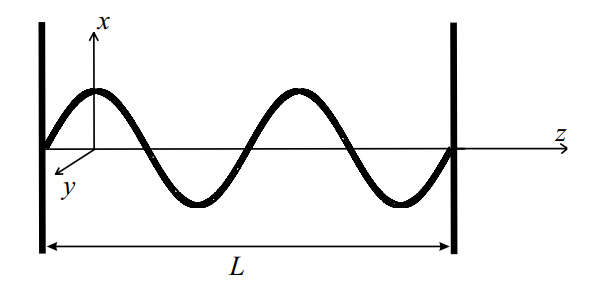
\includegraphics[scale=0.5]{em}
\end{figure}


Suppose that the field is a standing wave which vanishes on the boundary and is polarized in the $x$-direction. We also assume there is no source of radiation such as a charge or a current. The electric field then can be written as
\begin{align}
\mathbf{E}(\mathbf{r},t) = \mathbf{e}_xE_x(z,t)
\end{align}
where $\mathbf{e}_x$ is the polarization vector. The Maxwell's equations without source are
\begin{align}
\curl{\mathbf{E}} &= -\f{\p \mathbf{B}}{\p t}\\
\curl{\mathbf{B}} &= \mu_0\epsilon_0\f{\p \mathbf{E}}{\p t}\\
\div{\mathbf{E}} &= 0\\
\div{\mathbf{B}} &= 0.
\end{align}

A single-mode field satisfying Maxwell’s equations and the boundary conditions is given by
\begin{align}
E_x(z,t) = \lp \f{2\omega^2}{V\epsilon_0} \rp^{1/2} q(t)\sin(kz).
\end{align}
$\omega$ is the frequency, $k = \omega/c$ is the wavenumber. The allowed frequencies are
\begin{align}
\omega_m = c\f{m \pi}{L},\hspace{0.5cm}  =1,2,\dots
\end{align} 
$V$ is the effective volume of the cavity and $q(t)$ is the time-dependent factor having the dimension of length. The magnetic field, from the second Maxwell equation, is
\begin{align}
\mathbf{B}(\mathbf{r},t) = \mathbf{e}_yB_y(z,t)
\end{align}
where
\begin{align}
B_y(z,t) = \lp \f{\mu_0\epsilon_0}{k} \rp\lp \f{2\omega^2}{V\epsilon_0} \rp^{1/2}\dot{q}(t)\cos(kz).
\end{align}
It will become clear that $q(t)$ plays the role of canonical position, and $\dot{q}(t) = p(t)$ plays the role of canonical momentum. The classical field energy (or the Hamiltonian $\ham$) of this single-mode field is then given by
\begin{align}
\ham &= \f{1}{2}\int\,dV \lb \epsilon_0 \mathbf{E}^2(\mathbf{r},t) + \f{1}{\mu_0}\mathbf{B}^2(\mathbf{r},t) \rb\\
&= \f{1}{2}\int\,dV \lb \epsilon_0 E^2_x(z,t) + \f{1}{\mu_0}B_y^2(z,t) \rb
\end{align}
It turns out that (for $p(t) = \dot{q}(t)$), we have
\begin{align}
\boxed{\ham = \f{1}{2}\lp p^2 + \omega^2q^2 \rp}
\end{align} 
Now, we notice that we have the canonical variables $q$ and $p$. When we promote these variables to operators (so we can quantize the fields), these operators must satisfy the canonical commutation relation
\begin{align}
[\hat{q}, \hat{p}] = i\hbar \hat{\Id}
\end{align}
We rewrite the fields and the Hamiltonian as operators:
\begin{align}
\hat{E}_x(z,t) &= \lp \f{2\omega^2}{V\epsilon_0} \rp^{1/2} \hat{q}(t)\sin(kz)\\
\hat{B}_y(z,t) &= \lp \f{\mu_0\epsilon_0}{k} \rp\lp \f{2\omega^2}{V\epsilon_0} \rp^{1/2}\hat{p}(t)\cos(kz).\\
\hat{\ham} &= \f{1}{2}\lp \hat{p}^2 + \omega^2\hat{q}^2 \rp.
\end{align}
The operators $\hat{q}$ and $\hat{p}$ correspond to observables because they are Hermitian. We can also introduce creation ($\hat{a}^\dagger$) and annihilation ($\hat{a}$) operators through combining $\hat{q}$ and $\hat{p}$:
\begin{align}
\hat{a} &= (2\hbar\omega)^{-1/2}(\omega\hat{q} + i\hat{p})\\
\hat{a}^\dagger &= (2\hbar\omega)^{-1/2}(\omega\hat{q} - i\hat{p})
\end{align}
It is easy to show that the electric and magnetic field operators then become
\begin{align}
\hat{E}_x(z,t) &= \mathcal{E}_0(\hat{a} + \hat{a}^\dagger)\sin(kz)\\
\hat{B}_y(z,t) &= \mathcal{B}_0\f{1}{i}(\hat{a} - \hat{a}^\dagger)\cos(kz)
\end{align}
where
\begin{align}
\mathcal{E}_0 = \sqrt{\f{\hbar\omega}{\epsilon_0 V}}, \hspace{0.5cm}
\mathcal{B}_0 = \lp\f{\mu_0}{k}\rp\sqrt{\f{\epsilon_0\hbar\omega^3}{V}}
\end{align}
represents respectively the electric and magnetic field ``per photon.'' We notice that
\begin{align}
[\hat{a}, \hat{a}^\dagger] = \hat{\Id}
\end{align}
so the Hamiltonian takes the form
\begin{align}
\boxed{\hat{\ham} = \hbar\omega\lp \hat{a}^\dagger\hat{a} + \f{1}{2} \rp}
\end{align}

Now, what is the time dependent of these new operators? For an arbitrary operator $\hat{O}$, Heisenberg equation reads
\begin{align}
\f{d\hat{O}}{dt} = \f{i}{\hbar}[\hat{H},\hat{O}].
\end{align}
For the annihilation operator, this becomes
\begin{align}
\f{d\hat{a}}{dt} = \f{i}{\hbar}\lb \hbar\omega\lp \hat{a}^\dagger\hat{a} + \f{1}{2} \rp, \hat{a} \rb = -i\omega \hat{a}.
\end{align}
Thus,
\begin{align}
\boxed{\hat{a}(t) = \hat{a}(0)e^{i\omega t}}
\end{align}
Similarly for the creation operator, we have
\begin{align}
\boxed{\hat{a}^\dagger(t) = \hat{a}^\dagger(0) e^{i\omega t}}
\end{align}

Now, let $\ket{n}$ denote an energy eigenstate of the single mode field corresponding to energy $E_n$, then 
\begin{align}
\hat{\ham}\ket{n} = \hbar\omega\lp \hat{a}^\dagger\hat{a} + \f{1}{2} \rp\ket{n} = E_n\ket{n}.
\end{align}
Applying the creation operator $\hat{a}^\dagger$ from the left we have
\begin{align}
\hbar\omega\lp \hat{a}^\dagger\hat{a}^\dagger\hat{a} + \f{1}{2}\hat{a}^\dagger \rp\ket{n} = E_n\hat{a}^\dagger\ket{n}.
\end{align}
Using the commutation relation, we can write 
\begin{align}
\hat{a}\hat{a}^\dagger = \hat{\Id} + \hat{a}^\dagger\hat{a}.
\end{align}
Thus,
\begin{align}
E_n\hat{a}^\dagger\ket{n} &= \hbar\omega\lp \hat{a}^\dagger[-\hat{\Id} + \hat{a}\hat{a}^\dagger] + \f{1}{2}\hat{a}^\dagger \rp\ket{n}\\
&= \hbar\omega\lp -\hat{a}^\dagger + \hat{a}^\dagger\hat{a}\hat{a}^\dagger + \f{1}{2}\hat{a}^\dagger \rp\ket{n}\\
&= \hbar\omega\lp -\hat{\Id} + \hat{a}^\dagger\hat{a} + \f{1}{2}  \rp\hat{a}^\dagger\ket{n}.
\end{align}
This says we have a new eigen-equation:
\begin{align}
(E_n + \hbar\omega) \hat{a}^\dagger\ket{n} = \hbar\omega\lp \hat{a}^\dagger\hat{a} + \f{1}{2} \rp\hat{a}^\dagger\ket{n}
\end{align}
or equivalently,
\begin{align}
\boxed{\hat{H}\lb\hat{a}^\dagger\ket{n}\rb = (E_n + \hbar\omega)\lb\hat{a}^\dagger\ket{n}\rb}
\end{align}
This is the eigenvalue problem for the eigenstate $\hat{a}^\dagger\ket{n}$ with the energy eigenvalue $E_n + \hbar\omega$. It is clear now why $\hat{a}^\dagger$ is called the creation operator: it creates a ``quantum'' energy $\hbar\omega$. On the other hand, we can also show that
\begin{align}
\boxed{\hat{H}\lb\hat{a}\ket{n}\rb = (E_n - \hbar\omega)\lb\hat{a}\ket{n}\rb} 
\end{align}
It is clear that the operator $\hat{a}$ annihilates a quantum of energy. Now, because for the least energetic eigenstate
\begin{align}
\hat{a}\ket{0} = 0,
\end{align}
the Hamiltonian of the annihilation of the least energetic eigenstate is 
\begin{align}
\hat{\ham}\lb \hat{a}\ket{0} \rb  = (E_0 - \hbar\omega)\lb \hat{a}\ket{0}\rb = 0.
\end{align}
Therefore,
\begin{align}
\hat{\ham}\ket{0} = \hbar\omega\lp \hat{a}^\dagger\hat{a} + \f{1}{2}\rp\ket{0} = \f{1}{2}\hbar\omega\ket{0} = E_0\ket{0}.
\end{align}
Or equivalently, the zero-point energy is 
\begin{align}
E_0 = \hbar\omega
\end{align}
and the energy eigenvalues $E_{n+1} = E_n + \hbar\omega$ are
\begin{align}
\boxed{E_n = \hbar\lp n + \f{1}{2}\rp}
\end{align}
Note that this is just like the energy levels for the harmonic oscillator in an infinite well. Now, we observe that
\begin{align}
\hat{\ham}\ket{n} = \hbar\omega\lp \hat{a}^\dagger\hat{a} + \f{1}{2}\rp \ket{n} = E_n\ket{n} = \hbar\omega\lp n + \f{1}{2} \rp\ket{n},
\end{align}
i.e.,
\begin{align}
\hat{a}^\dagger\hat{a}\ket{n} = n\ket{n}.
\end{align}
It makes sense to call $\hat{a}^\dagger\hat{a}$ the ``number operator'' $\hat{n}$, so that 
\begin{align}
\hat{n}\ket{n} = n\ket{n}.
\end{align}
Next, the eigenstates must be normalized according to $\braket{n} = 1$. For the state $\hat{a}\ket{n}$ we have
\begin{align}
\hat{a}\ket{n} = c_n\ket{n-1}.
\end{align}
Taking the inner product with itself we have
\begin{align}
\lp\bra{n}\hat{a}^\dagger\rp\lp\hat{a}\ket{n}\rp &= \bra{n}\hat{a}^\dagger\hat{a}\ket{n}\\
&= \bra{n}\hat{n}\ket{n}\\
&= n\braket{n}\\
&= \bra{n-1}c_n^*c_n\ket{n-1}.
\end{align}
This says $n = \abs{c_n}^2$. So we have
\begin{align}
\boxed{\hat{a}\ket{n} = \sqrt{n}\ket{n-1}}
\end{align}
Similarly, 
\begin{align}
\boxed{\hat{a}^\dagger\ket{n} = \sqrt{n+1}\ket{n+1}}
\end{align}
This says that $\ket{n}$ can be generated from the $\ket{0}$ state by applying the creation operator $\hat{a}^\dagger$ appropriately many times with the appropriate normalization:
\begin{align}
\boxed{\ket{n} = \f{{\lp\hat{a}^\dagger\rp}^n}{\sqrt{n!}}\ket{0}}
\end{align}


Next, because the eigenstates are orthonormal ($\braket{n'}{n} = \delta_{n'n}$ and $\braket{n}=1$) and form a complete set, i.e.,
\begin{align}
\sum^\infty_{n=0}\ket{n}\bra{n} = 1,
\end{align} 
the only non-vanishing matrix elements of the annihilation and creation operators are
\begin{align}
&\bra{n-1}\hat{a}\ket{n} = \sqrt{n}\braket{n-1} = \sqrt{n} \\
&\bra{n+1}\hat{a}^\dagger\ket{n} = \sqrt{n+1}\braket{n+1} = \sqrt{n+1}
\end{align}



\subsection{Quantum Fluctuations of a Single-mode Field}
Recall the electric field operator
\begin{align}
\hat{E}_x(z,t) &= \mathcal{E}_0(\hat{a} + \hat{a}^\dagger)\sin(kz).
\end{align}
The mean field is zero:
\begin{align}
\bra{n}\hat{E}_x(z,t)\ket{n} = \mathcal{E}_0\sin(kz)[\underbrace{\bra{n}\hat{a}\ket{n}}_{0} + \underbrace{\bra{n}\hat{a}^\dagger\ket{n}}_{0}] = 0
\end{align}
by orthonormality. However, the mean of the square of the field is not zero:
\begin{align}
\bra{n}\hat{E}^2_x(z,t)\ket{n} &= \mathcal{E}^2_0\sin^2(kz)\bra{n}{\lp\hat{a}^\dagger\rp}^2 + \hat{a}^2 + \hat{a}^\dagger\hat{a}+ \hat{a}\hat{a}^\dagger\ket{n}\\
&= \mathcal{E}^2_0\sin^2(kz)\bra{n} 2\hat{a}^\dagger\hat{a} + 1  \ket{n} \\
&= 2\mathcal{E}^2_0\sin^2(kz)\lp n + \f{1}{2}\rp.
\end{align}
So, the fluctuations in the field for the state $\ket{n}$ may be characterized by the variance
\begin{align}
\text{Var}[\hat{E}_x(z,t)] &= \text{E}[\hat{E}^2_x(z,t)] - \text{E}^2[\hat{E}_x(z,t)] \\ &= 2\mathcal{E}^2_0\sin^2(kz)\lp n + \f{1}{2}\rp.
\end{align}
And so the uncertainty of the field for the state $\ket{n}$ is
\begin{align}
\boxed{\sigma[\hat{E}_x(z,t)]= \sqrt{2\mathcal{E}_0}\sin(kz)\sqrt{n+ \f{1}{2}}}
\end{align}
Now, note that even at $n=0$, the field still has fluctuations. These are called ``vacuum fluctuations.'' Now the number states $\ket{n}$ are taken to represent a state of the field containing $n$ photons. Yet as we have seen, the average field is zero. This is all in accordance with the uncertainty principle because the number operator $\hat{n} = \hat{a}^\dagger\hat{a}$ does not commute with the electric field:
\begin{align}
[\hat{n}, \hat{E}_x] = \mathcal{E}_0 \sin(kz)(\hat{a}^\dagger - \hat{a}).
\end{align}
Thus $\hat{n}$ and $\hat{E}_x$ are complementary quantities for which their respective uncertainties obey the inequality
\begin{align}
\sigma[ n ]\cdot \sigma[ E_x ]\geq \f{1}{2}\mathcal{E}_0\abs{\sin(kz)}\abs{\langle \hat{a}^\dagger - \hat{a}\rangle}
\end{align}
This says that if the field is accurately known, then the number of photons in uncertain. 



\subsection{Quadrature Operators for a Single-mode Field}

When we explicitly include the time dependence of the electric field operator we have
\begin{align}
\hat{E}_x = \mathcal{E}_0 (\hat{a}e^{-\omega t} + \hat{a}^\dagger e^{i\omega t})\sin(kz)
\end{align}
where
\begin{align}
\hat{a}(0) \equiv \hat{a} \hspace{0.5cm} \hat{a}^\dagger(0) \equiv \hat{a}^\dagger.
\end{align}

Next, we define quadrature operators:
\begin{align}
&\hat{X}_1 = \f{1}{2}(\hat{a} + \hat{a}^\dagger)\\
&\hat{X}_2 = \f{1}{2i}(\hat{a} - \hat{a}^\dagger).
\end{align}
With these definitions, we rewrite the time-dependent electric field operator as
\begin{align}
\hat{E}_x(t) = 2\mathcal{E}_0\sin(kz)[\hat{X}_1 \cos(\omega t) + \hat{X}_2\sin(\omega t)].
\end{align}

We observe that $\hat{X}_1$ and $\hat{X}_2$ are associated with field amplitudes oscillating $\pi/2$ out of phase. Essentially, $\hat{X}_1$ and $\hat{X}_2$ are position and momentum operators, only scaled to be dimensionless. These operators satisfy the commutation relation
\begin{align}
[\hat{X}_1, \hat{X}_2] = \f{i}{2},
\end{align}
which one can easily check. Next, by definition we have
\begin{align}
\bra{n}\hat{X}_1\ket{n} = \bra{n}\hat{X}_2\ket{n} = 0.
\end{align}
However, 
\begin{align}
\bra{n}\hat{X}_1^2\ket{n} &= \f{1}{4}\bra{n} \hat{a}^2 + (\hat{a}^\dagger)^2 + \hat{a}^\dagger\hat{a} + \hat{a}\hat{a}^\dagger \ket{n}\\
&= \f{1}{4}\bra{n} 2\hat{a}^\dagger\hat{a} + 1 \ket{n}\\
&= \f{1}{4}(2n + 1).
\end{align}
Similarly, 
\begin{align}
\bra{n}\hat{X}_2^2\ket{n} = \f{1}{4}(2n + 1).
\end{align}
Thus for a number state, the uncertainties in both quadratures are the same and furthermore the vacuum state ($n = 0$) minimizes the uncertainty product since
\begin{align}
\text{Var}[\hat{X}_1] = \text{Var}[\hat{X}_2] = \f{1}{4}.
\end{align}

From this section, we learn that the quanta of the single-mode cavity field are the excitations of energy in discrete amounts of $\hbar\omega$. These quantas (or photons) are not localized particles but rather are spread out over the entire mode volume. 

















\subsection{Multimode Fields}

Now we generalize our results for the single-mode field to multi-mode fields. We again assume that there is no source of radiation. Let the vector potential $\mathbf{A}(\mathbf{r},t)$ be given such that
\begin{align}\label{gauge}
\div{\mathbf{A}(\mathbf{r},t)} = 0.
\end{align}
The vector potential gives the electric and magnetic fields by
\begin{align}\label{EB}
\mathbf{E}(\mathbf{r},t) &= -\f{\p \mathbf{A}(\mathbf{r},t)}{\p t}\\
\mathbf{B}(\mathbf{r},t) &= \curl{\mathbf{A}(\mathbf{r},t)}.
\end{align}
The vector potential satisfies the wave equation
\begin{align}\label{waves}
\laplacian{\mathbf{A}(\mathbf{r},t)} - \f{1}{c^2}\f{\p^2 \mathbf{A}(\mathbf{r},t)}{\p t^2} = 0.
\end{align}

We now assume free space is a cubic cavity with perfectly reflecting walls of length $L$. We assume that $L \to \infty$, i.e., $L$ is much larger than the wavelength of the field. This allows us to impose boundary conditions:
\begin{align}
&e^{ik_x x} = e^{ik_x(x+L)}\\
&e^{ik_y x} = e^{ik_y(y+L)}\\
&e^{ik_z x} = e^{ik_z(z+L)}.
\end{align}
It follows that
\begin{align}
&k_x = \lp \f{2\pi}{L} \rp m_x, \hspace{0.5cm} m_x = 0, \pm 1, \pm 2, \dots\\
&k_y = \lp \f{2\pi}{L} \rp m_y, \hspace{0.5cm} m_y = 0, \pm 1, \pm 2, \dots\\
&k_z = \lp \f{2\pi}{L} \rp m_z, \hspace{0.5cm} m_z = 0, \pm 1, \pm 2, \dots
\end{align}
The wave vector is then
\begin{align}
\mathbf{k} = \f{2\pi }{L}\begin{bmatrix}
m_x\\m_y\\m_z
\end{bmatrix}.
\end{align}
The magnitude of this vector is related to the frequency $\omega_k$ according to $k = \omega_k / c$. A set of integers $(m_x , m_y , m_z)$ specifies a normal mode of the field (apart from polarization), the number of modes being infinite but denumerable. The total number of modes in the intervals $\Delta m_x, \Delta m_y, \Delta m_z$ is
\begin{align}
\Delta m = \Delta m_x \Delta m_y \Delta m_z = 2\lp \f{L}{2\pi} \rp^3 \Delta k_x \Delta k_y \Delta k_z
\end{align}
where the factor of $2$ takes into account two independent modes of polarization. With the assumption that $L$ is very large compared to the wavelengths, this becomes
\begin{align}
dm = 2\lp \f{V}{8\pi^3} \rp d k_x d k_y d k_z.
\end{align}
In spherical coordinates, 
\begin{align}
\mathbf{k} = k(\sin\theta\cos\phi, \sin\theta\sin\phi, \cos\theta),
\end{align}
and 
\begin{align}
dm = 2\lp \f{V}{8\pi^3} \rp k^2 \, dk d\Omega
\end{align}
where
\begin{align}
d\Omega = \sin\theta \,d\theta d\phi.
\end{align}
With $k = \omega_k/c$,
\begin{align}
dm = 2\lp \f{V}{8\pi^3} \rp \f{\omega^2_k}{c^3} \, d\omega_k d\Omega.
\end{align}
Integrating over all solid angles gives $\int \,d\Omega = 4\pi$, so the number of modes in all directions from $k \to k + dk$ is 
\begin{align}
2\lp \f{V}{8\pi^3} \rp k^2 \cdot (4\pi) \, dk = V \f{k^2}{\pi^2}\,dk = V \rho_k \,dk
\end{align}
where $\rho_k = k^2/\pi^2$ and $\rho_k \,dk$ is the number of modes per unit volume. Integrating in the same fashion but with $\omega_k$ gives the number of modes in all directions from $\omega_k \to \omega_k + d\omega_k$:
\begin{align}
V \lp \f{\omega_k^2}{\pi^2 c^3} \rp\,d\omega_k = V \rho(\omega_k)\,d\omega_k
\end{align}
where now $\rho(\omega_k)$ is also the mode density. \\

The vector potential can be written as a superposition on plane waves in the form
\begin{align}
\mathbf{A}(\mathbf{r},t) = \sum_{\mathbf{k},s}\mathbf{e}_{\mathbf{k}s} \lb A_{\mathbf{k}s}(t)e^{i\mathbf{k}\cdot\mathbf{r}} + A_{\mathbf{k}s}^* e^{-i\mathbf{k}\cdot \mathbf{r}} \rb 
\end{align}
where $A_{\mathbf{k}s}$ is the complex amplitude of the field and $\mathbf{e}_{\mathbf{k}s}$ is a real polarization vector. The sum over $k$ simply means the sum over the set of integers $(m_x , m_y , m_z)$ and the sum over $s$ is the sum over the two independent polarizations. These polarizations must be orthogonal:
\begin{align}
\mathbf{e}_{\mathbf{k}s} \cdot \mathbf{e}_{\mathbf{k}s'} = 0
\end{align}
and the \textit{transversality} condition must be satisfied:
\begin{align}
\mathbf{k}\cdot\mathbf{e}_{\mathbf{k}s} = 0,
\end{align}
which is just says that the polarization is orthogonal to the propagation. The polarization vectors $\mathbf{e}_{\mathbf{k}1}$ and $\mathbf{e}_{\mathbf{k}2}$ form a right-handed system:
\begin{align}
\mathbf{e}_{\mathbf{k}1}\times \mathbf{e}_{\mathbf{k}2} = \f{\mathbf{k}}{\abs{\mathbf{k}}} = \mathbf{\kappa}.
\end{align}
In free space, we make the transition from ``discrete'' modes to a continuum of modes, thus the sum becomes an integral:
\begin{align}
\sum_{\mathbf{k}} \to \f{V}{\pi^2}\int k^2\,dk.
\end{align}
From \eqref{gauge} and \eqref{waves} and $\omega_k = kc$, we get
\begin{align}
\f{d^2 A_{\mathbf{k}s}}{dt^2} + \omega_k^2 A_{\mathbf{k}s} =0. 
\end{align}
The solution to this is of course
\begin{align}
A_{\mathbf{k}s}(t) = A_{\mathbf{k}s}(0)e^{-i\omega_k t} = A_{\mathbf{k}s}e^{-i\omega_k t}.
\end{align}
From this and \eqref{EB} we can derive the electric and magnetic fields:
\begin{align}
&\mathbf{E}(\mathbf{r},t) = i\sum_{\mathbf{k},s} \omega_k \mathbf{e}_{\mathbf{k}s} \lb A_{\mathbf{k}s}e^{i(\mathbf{k}\cdot\mathbf{r} - \omega_k t)} - A_{\mathbf{k}s}^* e^{-i(\mathbf{k}\cdot\mathbf{r} - \omega_k t)}\rb\\
&\mathbf{B}(\mathbf{r},t) = \f{i}{c}\sum_{\mathbf{k},s} \omega_k (\mathbf{\kappa} \times \hat{\mathbf{e}}_{\mathbf{k}s}) \lb A_{\mathbf{k}s}e^{i(\mathbf{k}\cdot\mathbf{r} - \omega_k t)} - A_{\mathbf{k}s}^* e^{-i(\mathbf{k}\cdot\mathbf{r} - \omega_k t)}\rb.
\end{align}
The electromagnetic Hamiltonian is given by
\begin{align}
\ham = \f{1}{2}\int_V \lp \epsilon_0 \mathbf{E}\cdot \mathbf{E} + \f{1}{\mu_0} \mathbf{B}\cdot\mathbf{B} \rp\,dV.
\end{align}
The periodic boundary conditions result in
\begin{align}
\int_0^L e^{\pm i k_x x}\,dx = \begin{cases}
L,\hspace{0.5cm} k_x = 0\\
0,\hspace{0.5cm} k_x \neq 0
\end{cases}
\end{align}
same for $y$ and $z$. Collectively we write this as
\begin{align}
\int_V e^{\pm i(\mathbf{k} - \mathbf{k}')\cdot\mathbf{r}} \, dV = \delta_{\mathbf{k}\mathbf{k}'}V.
\end{align}
So the contribution to the Hamiltonian from the electric field is
\begin{align}
\f{1}{2}\int_V \epsilon_0 \mathbf{E}\cdot\mathbf{E}\,dV = &\epsilon_0 V \sum_{\mathbf{k}s}\omega_k^2 A_{\mathbf{k}s}(t)A^*_{\mathbf{k}s}(t) \\
& - \underbrace{\f{1}{2}\epsilon_0 V\sum_{\mathbf{k}ss'}\omega^2_k \mathbf{e}_{\mathbf{k}s}\cdot \mathbf{e}_{-\mathbf{k}s'}\lb A_{\mathbf{k}s}(t)A_{\mathbf{k}s'}(t) + A^*_{\mathbf{k}s}(t)A^*_{-\mathbf{k}s'}(t) \rb}_R.
\end{align}
To obtain the magnetic contribution we use the identity
\begin{align}
(\mathbf{A}\times \mathbf{B})\cdot (\mathbf{C}\times \mathbf{D}) = (\mathbf{A}\cdot\mathbf{C})(\mathbf{B}\cdot \mathbf{D}) - (\mathbf{A}\cdot\mathbf{D})(\mathbf{B}\cdot\mathbf{C}).
\end{align}
This gives
\begin{align}
(\mathbf{\kappa}\times \mathbf{e}_{\mathbf{k}s})\cdot(\mathbf{\kappa}\times \mathbf{e}_{\mathbf{k}s'}) &= \delta_{ss'}\\
(\mathbf{\kappa}\times \mathbf{e}_{\mathbf{k}s})\cdot(-\mathbf{\kappa}\times \mathbf{e}_{-\mathbf{k}s'}) &= -\mathbf{e}_{\mathbf{k}s}\cdot \mathbf{e}_{-\mathbf{k}s'}.
\end{align}
With this we get the contribution from the magnetic field
\begin{align}
\f{1}{2}\int_V \f{1}{\mu_0}\mathbf{B}\cdot\mathbf{B}\,dV = &\epsilon_0 V \sum_{\mathbf{k}s}\omega^2_k A_{\mathbf{k}s}(t)A^*_{\mathbf{k}s}(t) + R.
\end{align}
Thus the Hamiltonian is
\begin{align}
\ham &= 2\epsilon_0 V \sum_{\mathbf{k}s} \omega^2_k A_{\mathbf{k}s}(t)A^*_{\mathbf{k}s}(t)\\
&= 2\epsilon_0 V \sum_{\mathbf{k}s} \omega^2_k A_{\mathbf{k}s}(0)e^{-i\omega_k t}A^*_{\mathbf{k}s}(0)e^{i\omega_k t}\\
&= 2\epsilon_0 V \sum_{\mathbf{k}s} \omega^2_k A_{\mathbf{k}s}A^*_{\mathbf{k}s}.
\end{align}
To quantize the field, the canonical variables $q_{\mathbf{k}s}$ and $p_{\mathbf{k}s}$ must be introduced:
\begin{align}
A_{\mathbf{k}s} &= \f{1}{2\omega_k \sqrt{\epsilon_0 V}}[\omega_k q_{\mathbf{k}s} + ip_{\mathbf{k}s}]\\
A^*_{\mathbf{k}s} &= \f{1}{2\omega_k \sqrt{\epsilon_0 V}}[\omega_k q_{\mathbf{k}s} - ip_{\mathbf{k}s}]
\end{align}
such that when we can re-write the Hamiltonian as
\begin{align}
\ham = \f{1}{2}\sum_{\mathbf{k}s} \lp p^2_{\mathbf{k}s} + \omega_k^2q_{\mathbf{k}s}^2\rp.
\end{align}

To quantize the field, we promote these canonical variables to operators:
\begin{align}
\boxed{\hat{\ham} = \f{1}{2}\sum_{\mathbf{k}s} \lp \hat{p}^2_{\mathbf{k}s} + \omega_k^2\hat{q}_{\mathbf{k}s}^2\rp}
\end{align}
where 
\begin{align}
\lb\hat{q}_{\mathbf{k}s}, \hat{q}_{\mathbf{k}'s'}\rb &= 0 = \lb\hat{p}_{\mathbf{k}s}, \hat{p}_{\mathbf{k}'s'}\rb \\
\lb\hat{q}_{\mathbf{k}s}, \hat{p}_{\mathbf{k}'s'}\rb &= i\hbar\delta_{\mathbf{kk}'}\delta_{ss'}.
\end{align}
The annihilation and creation operators are defined in a similar fashion as in the case of a single-mode field:
\begin{align}
\hat{a}_{\mathbf{k}s} &= (2\hbar\omega_k)^{-1/2}(\omega_k \hat{q}_{\mathbf{k}s} + i\hat{p}_{\mathbf{k}s})\\
\hat{a}^\dagger_{\mathbf{k}s} &= (2\hbar\omega_k)^{-1/2}(\omega_k \hat{q}_{\mathbf{k}s} - i\hat{p}_{\mathbf{k}s})
\end{align}
which satisfy
\begin{align}
\lb\hat{a}_{\mathbf{k}s}, \hat{a}_{\mathbf{k}'s'}\rb &= 0 = \lb\hat{a}^\dagger_{\mathbf{k}s}, \hat{a}^\dagger_{\mathbf{k}'s'}\rb\\
\lb \hat{a}_{\mathbf{k}s}, \hat{a}^\dagger_{\mathbf{k}'s'}  \rb &= \delta_{\mathbf{kk}'}\delta_{ss'}.
\end{align}
Finally, we define a similar operator for the mode $\mathbf{k}s$ as the ``number'' operator before
\begin{align}
\hat{n}_{\mathbf{k}s} = \hat{a}^\dagger_{\mathbf{k}s} \hat{a}_{\mathbf{k}s}.
\end{align}
With these, the Hamiltonian (operator) can be written as
\begin{align}
\hat{\ham} = \sum_{\mathbf{k}s}\hbar\omega_k \lp \hat{a}_{\mathbf{k}s}^\dagger\hat{a}_{\mathbf{k}s} + \f{1}{2} \rp = \sum_{\mathbf{k}s} \omega_k \lp \hat{n}_{\mathbf{k}s} +\f{1}{2} \rp.
\end{align}
For simplicity, we associate a $j^\text{th}$ mode with $\mathbf{k}_js_j$. We let
\begin{align}
\hat{a}_{\mathbf{k}_j s_j} &\equiv \hat{a}_j\\
\hat{a}^\dagger_{\mathbb{k}_j s_j} &\equiv \hat{a}^\dagger_j\\
\hat{n}_{\mathbf{k}_j s_j} &\equiv \hat{n}_j.
\end{align}
Now we can write the Hamiltonian as
\begin{align}
\boxed{\hat{\ham} = \sum_j \hbar\omega_j \lp \hat{n}_j + \f{1}{2} \rp}
\end{align}

A multimode photon number state is a (tensor) product of the number states $\ket{n_{\mathbf{k}s}} \equiv \ket{n_j}$ of all the modes which we write as
\begin{align}
\ket{n_1}\ket{n_2}\ket{n_3}\dots \equiv \ket{n_1n_2n_3\dots} = \ket{\{ n_j \}}.
\end{align}
This is an eigenstate of the Hamiltonian:
\begin{align}
\hat{\ham}\ket{\{ n_j \}} = E\ket{\{ n_j \}}.
\end{align}
We can show that energy eigenvalue is
\begin{align}
\boxed{E = \sum_j \hbar\omega_j \lp n_j + \f{1}{2} \rp}
\end{align}
Because the Hamiltonian is Hermitian (as always) the eigenstates are orthogonal:
\begin{align}
\bra{n_1n_2n_3\dots}\ket{n'_1n'_2n'_3\dots} = \delta_{n_1n'_1}\delta_{n_2n'_2}\delta_{n_3n'_3}\dots
\end{align}
The actions of the annihilation and creation operator are as expected and similar to what we have seen before:
\begin{align}
&\boxed{\textbf{Annihilation: } \hat{a}_j \ket{n_1,n_2,\dots,n_j,\dots} = \sqrt{n_j}\ket{n_1,n_2,\dots,n_j - 1,\dots}}\\
&\boxed{\textbf{Creation: } \hat{a}^\dagger_j \ket{n_1,n_2,\dots,n_j,\dots} = \sqrt{n_j + 1}\ket{n_1,n_2,\dots,n_j + 1,\dots}}
\end{align}


The vacuum multimode is denoted
\begin{align}
\ket{\{ 0 \}} = \ket{0_10_20_3\dots 0_j\dots}
\end{align}
for which
\begin{align}
\hat{a}_j \ket{\{ 0 \}} = 0 \hspace{0.5cm} \text{for all }j.
\end{align}
Once again, like in the single-mode case, a multimode number state can be generated by applying the creation operator. Any number state can be written as some creation operator applied to the multimode vacuum:
\begin{align}
\ket{\{ n_j \}} = \prod_{j} \f{(\hat{a}^\dagger_{j})^{n_j}}{\sqrt{n_j !}}\ket{\{ 0 \}}.
\end{align}

Now, we notice that the creation/annihilation operators $\hat{a}_{\mathbf{k}s}$/$\hat{a}^\dagger_{\mathbf{k}s}$ are very much like the vector potential amplitude $A_{\mathbf{k}s}$. Indeed, upon quantization of the field, the amplitudes can be promoted to operators as well:
\begin{align}
\hat{A}_{\mathbf{k}s} = \lp \f{\hbar}{2\omega_k \epsilon_0 V} \rp^{\f{1}{2}}\hat{a}_{\mathbf{k}s}.
\end{align}
With this, we are able to rewrite the vector potential, electric, and magnetic fields in terms of the creation and annihilation operators:
\begin{align}
&\hat{\mathbf{A}}(\mathbf{r},t) = \sum_{\mathbf{k}s}\lp\f{\hbar}{2\omega_k \epsilon_0 V}\rp^{\f{1}{2}} \mathbf{e}_{\mathbf{k}s} \lb \hat{a}_{\mathbf{k}s}e^{i(\mathbf{k}\cdot\mathbf{r} - \omega_k t)}
+ \hat{a}^\dagger_{\mathbf{k}s}e^{-i(\mathbf{k}\cdot\mathbf{r} - \omega_k t)}  \rb\\
&\hat{\mathbf{E}}(\mathbf{r},t) = i\sum_{\mathbf{k}s}\lp\f{\hbar\omega_k}{2\epsilon_0 V}\rp^{\f{1}{2}} \mathbf{e}_{\mathbf{k}s} \lb \hat{a}_{\mathbf{k}s}e^{i(\mathbf{k}\cdot\mathbf{r} - \omega_k t)}
- \hat{a}^\dagger_{\mathbf{k}s}e^{-i(\mathbf{k}\cdot\mathbf{r} - \omega_k t)}  \rb\\
&\hat{\mathbf{B}}(\mathbf{r},t) = \f{i}{c}\sum_{\mathbf{k}s} (\mathbf{\kappa} \times \mathbf{e}_{\mathbf{k}s})\lp\f{\hbar\omega_k}{2 \epsilon_0 V}\rp^{\f{1}{2}} \mathbf{e}_{\mathbf{k}s} \lb \hat{a}_{\mathbf{k}s}e^{i(\mathbf{k}\cdot\mathbf{r} - \omega_k t)}
- \hat{a}^\dagger_{\mathbf{k}s}e^{-i(\mathbf{k}\cdot\mathbf{r} - \omega_k t)}  \rb.
\end{align}



The annihilation and creation operators are to be understood as Heisenberg picture operators evaluated at $t=0$. The time-dependent annihilation operator for a free field is given by  
\begin{align}
\hat{a}_{\mathbf{k}s}(t) = \hat{a}_{\mathbf{k}s}(0)e^{-i\omega_k t}.
\end{align}
With this the electric field can be written as
\begin{align}
\hat{\mathbf{E}}(\mathbf{r},t) = i\sum_{\mathbf{k}s}\lp \f{\hbar\omega_k}{2\epsilon_0 V} \rp^{\f{1}{2}} \mathbf{e}_{\mathbf{k}s}   \lb \hat{a}_{\mathbf{k}s}(t)e^{i\mathbf{k}\cdot\mathbf{r}} - \hat{a}^\dagger_{\mathbf{k}s}(t)e^{-i\mathbf{k}\cdot\mathbf{r}} \rb.
\end{align}
where the $e^{\pm i \omega_k t}$ term is absorbed into the operator. Alternatively, the field can be written in a different form:
\begin{align}
\hat{\mathbf{E}}(\mathbf{r},t) = \hat{\mathbf{E}}^{(+)}(\mathbf{r},t) + \hat{\mathbf{E}}^{(-)}(\mathbf{r},t)
\end{align}
where
\begin{align}
\hat{\mathbf{E}}^{(+)}(\mathbf{r},t) = i\sum_{\mathbf{k}s}\lp \f{\hbar\omega_k}{2\epsilon_0 V} \rp^{\f{1}{2}}\mathbf{e}_{\mathbf{k}s}\hat{a}_{\mathbf{k}s}(t)e^{ i\mathbf{k}\cdot\mathbf{r}}.
\end{align}
Of course,
\begin{align}
\hat{\mathbf{E}}^{(+)}(\mathbf{r},t) = \lb \hat{\mathbf{E}}^{(-)}(\mathbf{r},t) \rb^\dagger.
\end{align}

Similar expressions can be obtained for the magnetic field. However, because the magnetic field is ``weaker'' than the electric field by a factor of $1/c$, we generally neglect the magnetic field in most matter-field interactions (as most interactions are through the electric dipole). $\hat{\mathbf{E}}^{(+)}(\mathbf{r},t)$ is called the \textit{positive frequency part} of the field as it contained all terms oscillate as $e^{-i\omega t}$ for $\omega > 0$. The opposite is for $\hat{\mathbf{E}}^{(-)}(\mathbf{r},t)$. We notice that $\hat{\mathbf{E}}^{(+)}(\mathbf{r},t)$ is a collective annihilation operator while the latter is a collective creation operator. \\

The last observation we make is the following. For a single-mode plane wave field the electric field is
\begin{align}
\hat{E}(\mathbf{r},t) = i\lp \f{\hbar\omega_k}{2\epsilon_0 V} \rp^{\f{1}{2}}\mathbf{e}_x\lb \hat{a} e^{i\mathbf{k}\cdot\mathbf{r} - i\omega t} - \hat{a}^\dagger e^{-i\mathbf{k}\cdot\mathbf{r} + i\omega t} \rb.
\end{align}
In most of quantum optics, the spatial variation of the field over the dimensions of the atomic system may be negligible, i.e., the length characteristic of the size of the atom is often much smaller than a typical wavelength:
\begin{align}
\f{\lambda}{2\pi} = \f{1}{\abs{k}} \gg \abs{\mathbf{r}_\text{atom}}.
\end{align}
With this, we can make an approximation:
\begin{align}
e^{\pm i\mathbf{k}\cdot\mathbf{r}} \approx 1 \pm i\mathbf{k}\cdot\mathbf{r}
\end{align}
which says we replace the exponential by unity for $\abs{\mathbf{r}}$ is negligible. Under this approximation, 
\begin{align}\label{dipoleE}
\boxed{\hat{\mathbf{E}}(\mathbf{r},t)  \approx \hat{\mathbf{E}}(t) = i \lp \f{\hbar\omega_k}{2\epsilon_0 V} \rp^{\f{1}{2}}\mathbf{e}_x \lb \hat{a}e^{-i\omega t} - \hat{a}^\dagger e^{i\omega t} \rb}
\end{align}
This is called the \textbf{``dipole'' approximation}. 




%\newpage
%
%\section{Coherent States}

\newpage

\section{Emission and Absorption of Radiation by Atoms}

\subsection{Atom-field interactions}
Suppose we have an atom in no external field. The Hamiltonian of an electron bound to this atom is given by
\begin{align}
\hat{\ham}_0 = \f{1}{2m}\hat{\mathbf{P}}^2 + V(r)
\end{align}
where $V(r)$ is the Coulomb interaction between the electron and nucleus and $r = \abs{\mathbf{r}}$ is the distance to the core. In the configuration space representation, 
\begin{align}
&\hat{\mathbf{P}} = -i \hbar \nabla\\
&\hat{\mathbf{r}}\ket{\mathbf{r}} = \mathbf{r}\ket{\mathbf{r}}.
\end{align}
The wave functions are given by
\begin{align}
\psi(\mathbf{r}) = \bra{\mathbf{r}}\ket{\psi}.
\end{align}
We assume that the energy eigenstates $\ket{k}$ of $\hat{\ham}_0$ satisfy the time-independent Schr\"{o}dinger equation:
\begin{align}
\hat{\ham}_0 \ket{\psi}_k^{(0)}(\mathbf{r}) = E_k \psi_k^{(0)}(\mathbf{r}) 
\end{align}
where 
\begin{align}
\bra{\mathbf{r}}\ket{k} = \psi_k^{(0)}(\mathbf{r})
\end{align}
are known. In the presence of external fields the Hamiltonian is modified to
\begin{align}
\hat{\ham}(\mathbf{r},t) = \f{1}{2m}\lb \hat{\mathbf{P}} + e\mathbf{A}(\mathbf{r} , t) \rb^2 - e\Phi(\mathbf{r},t) + V(r)
\end{align}
where $\mathbf{A}(\mathbf{r},t)$ and $\Phi(\mathbf{r},t)$ are the vector and scalar potentials, respectively, $-e$ is the electron charge. The electric and magnetic fields are given by
\begin{align}
&\mathbf{E}(\mathbf{r},t) = -\grad{\Phi(\mathbf{r},t)} - \f{\p \mathbf{A}(\mathbf{r},t)}{\p t}\\
&\mathbf{B}(\mathbf{r},t) = \curl{\mathbf{A}(\mathbf{r},t)}
\end{align}
which we can easily show to be invariant under the following gauge transformations
\begin{align}\label{gaug}
&\Phi'(\mathbf{r},t) = \Phi(\mathbf{r},t) - \f{\p \chi(\mathbf{r},t)}{\p t}\\
&\mathbf{A}'(\mathbf{r},t) = \mathbf{A}(\mathbf{r},t) + \grad{\chi(\mathbf{r},t)}.
\end{align}
The time-dependent Schr\"{o}dinger equation is
\begin{align}
\hat{\ham}(\mathbf{r},t)\psi(\mathbf{r},t) = i\hbar\f{\p \psi(\mathbf{r},t)}{\p t}.
\end{align}
To eventually simplify the form of the atom-field interaction, we define a unitary operator $\hat{R}$ such that
\begin{align}
\psi'(\mathbf{r},t) = \hat{R}\psi(\mathbf{r},t)
\end{align}
where
\begin{align}
\hat{\ham}' \psi'  = i\hbar \f{\p \psi'}{\p t}.
\end{align}
We can show that the new Hamiltonian relates to the old Hamiltonian as 
\begin{align}
\hat{\ham}' = \hat{R}\hat{\ham}\hat{R}^\dagger + i\hbar \f{\p \hat{R}}{\p t}\hat{R}^\dagger.
\end{align}
Our goal is to choose 
\begin{align}
\hat{R} = e^{-ie\chi(\mathbf{r},t)/\hbar},
\end{align}
so that with $\hat{\mathbf{P}}^2 = -i\hbar \nabla$:
\begin{align}
\hat{\ham}' =\f{1}{2m}\lb \hat{\mathbf{P}}^2 + e\mathbf{A}' \rb^2 - e\Phi' + V(r),
\end{align}
where the new vector and scalar potentials $\mathbf{A}'$ and $\Phi'$ depend on the gauge field $\chi$ as \eqref{gaug}. This form of the Hamiltonian is not desirable because of the interaction terms $\hat{\mathbf{P}} \cdot \mathbf{A}$ and $\mathbf{A}^2$. To remedy this, we can first make a definite choice of gauge, namely the Coulomb gauge, for which $\Phi = 0$ and $\div{\mathbf{A}} = 0$. Now with $\mathbf{A'} = \mathbf{A} + \grad{\chi}$ and $\Phi' = \Phi - \p \chi / \p t = - \p \chi / \p t$, the new Hamiltonian has the form
\begin{align}\label{newHam}
\hat{\ham}' = \f{1}{2m}\lb \hat{\mathbf{P}} + e\lp\mathbf{A} + \grad{\chi}\rp \rb^2 + e\f{\p \chi}{\p t} +V(r).
\end{align}
The vector potential $\mathbf{A}$ for no sources near the atom satisfies the wave equation
\begin{align}
\laplacian{\mathbf{A}} - \f{1}{c^2}\f{\p^2 \mathbf{A}}{\p t^2} = 0,
\end{align}
whose solution is simply a wave propagating wave
\begin{align}
\mathbf{A} = \mathbf{A}_0 e^{i(\mathbf{k}\cdot\mathbf{x} - \omega t)} + c.c.
\end{align}
where $\abs{\mathbf{k}} = 2\pi/\lambda$ is the wave vector of the radiation. For $\abs{\mathbf{r}}$ a typical atomic length ($10^{-10}$ m) and $\lambda$ of typical optical wavelengths ($10^{-7}$ m), the product $\mathbf{k}\cdot\mathbf{r} \ll 1$ so that over the extend of the atom $\mathbf{A}$ can be taken to be uniform, i.e.,
\begin{align}
\mathbf{A}(\mathbf{r},t) \approx \mathbf{A}(t).
\end{align} 
This is very much like the idea we discussed before regarding the electric field $\mathbf{E}$ in the quantization of the EM field. This is also called the \textbf{dipole approximation}. Now, the Hamiltonian in \eqref{newHam} has coupled terms, and we would like to remove $\nabla \chi$ from the coupling between itself and $\mathbf{A}$ and between $\mathbf{A}$ and $\hat{\mathbf{P}}$. One very good way to do this is finding $\chi$ such that
\begin{align}
\nabla \chi = - \mathbf{A}(\mathbf{r},t) \approx \mathbf{A}(t).
\end{align}
Such a $\chi(\mathbf{r},t)$ is
\begin{align}
\chi(\mathbf{r},t) = - \mathbf{A}(t)\cdot \mathbf{r}.
\end{align}
With this choice, we have (since $\nabla \mathbf{r} = \mathbf{1}$)
\begin{align}
&\nabla \chi(\mathbf{r},t) = -\mathbf{A}(t)\\
&\f{\p \chi}{\p t}(\mathbf{r},t) = -\mathbf{r}\cdot \f{\p \mathbf{A}(t)}{\p t} = -\mathbf{r}\cdot \mathbf{E}(t).
\end{align}
The new Hamiltonian is now ``decoupled":
\begin{align}
\boxed{\hat{\ham}' = \underbrace{\f{1}{2m}\hat{\mathbf{P}}^2 + V(r)}_{\text{field-free}} \underbrace{-e\mathbf{r}\cdot \mathbf{E}(t)}_{\text{dipole int.}}}
\end{align}
This new Hamiltonian contains only one interaction term (within the dipole approximation) as opposed to two terms as before. $-e\mathbf{r}$ is called the \textbf{dipole moment}, denoted $\mathbf{d}$. We can of course promote it to an operator, so that the Hamiltonian in the presence of an external field can be written as
\begin{align}
\boxed{\hat{\ham} = \hat{\ham}_0 - \hat{\mathbf{d}}\cdot\mathbf{E}(t)}
\end{align}
where $\hat{\ham}_0 = \hat{\mathbf{P}}^2/2m + V(r)$ is of course the field-free Hamiltonian. 



\subsection{Interaction of an atom with a classical field}

So far we have not specified whether the interacting field is classical or quantum mechanical. The derivation we just looked at is valid for both classical and quantum fields. However, we will eventually show that the atom behaves differently in each case. 

Let us first look at the the atom-field interaction with a classical field. Suppose the field is given by
\begin{align}
\mathbf{E}(t) = \mathbf{E}_0 \cos(\omega t)
\end{align}
where the dipole approximation $\mathbf{k}\cdot\mathbf{r} \ll 1$ has already been made (so that the field is uniform over the atom). Suppose that $\omega$ is the frequency of the radiation, and the field is abruptly turned on at $t = 0$. Assume that the initial state of the atom is $\ket{i}$ where
\begin{align}
\hat{\ham}_0 \ket{i} = E_i\ket{i}. 
\end{align}
For time $t > 0$, the state vector $\ket{\psi}(t)$ is a linear combination of all uncoupled states $\ket{k}$:
\begin{align}\label{exp}
\ket{\psi(t)} = \sum_k C_k(t) e^{-iE_k t/\hbar}\ket{k}
\end{align}
where
\begin{align}
\sum_k \abs{C_k(t)}^2= 1.
\end{align}
The time-dependent Schro\"{o}dinger equation is
\begin{align}
i\hbar \f{\p \ket{\psi(t)}}{\p t} = \lp \hat{\ham}_0 + \hat{\ham}^{(I)} \rp\ket{\psi(t)}
\end{align}
where
\begin{align}
\hat{\ham}^{(I)} = -\hat{\mathbf{d}}\cdot\mathbf{E}(t).
\end{align}
Substituting the expansion \eqref{exp} into the time-dependent SE, them multiplying from the left by $\bra{l}e^{-E_l t/\hbar}$ gives
\begin{align}
i\hbar \bra{l}e^{-E_l t/\hbar} \f{\p}{\p t}\sum_k C_k(t) e^{-iE_k t/\hbar}\ket{k} = \bra{l}e^{-i E_l t/\hbar} \lp \hat{\ham}_0 + \hat{\ham}^{(I)} \rp \sum_k C_k(t) e^{-iE_k t/\hbar}\ket{k}.
\end{align}
This simplifies to 
\begin{align}
\dot{C}_l(t) - \f{i}{\hbar}\sum_k C_k(t)\bra{l}\hat{\ham}^{(I)}\ket{k} e^{-i (E_l - E_k)t\hbar}.
\end{align}
Defining
\begin{align}
\omega_l = \f{E_l - E_K}{\hbar}
\end{align}
as the transition frequencies between levels $l$ and $k$ gives a set of couple-first-order differential equations for the amplitudes
\begin{align}\label{dif}
\dot{C}_l(t)=  - \f{i}{\hbar}\sum_k C_k(t)\bra{l}\hat{\ham}^{(I)}\ket{k} e^{-i\omega_l t}.
\end{align}
The initial condition is $C_i(0) = 1$: $\ket{i}$ is the only state initially populated. As time goes forward, the population in $\ket{i}$ will decrease and move to some unpopulated $\ket{f}$. The probability of the transition $i \to f$ is given by
\begin{align}
P_{i\to f}(t) = C^*(f)C_f(t) = \abs{C_f(t)}^2. 
\end{align}
For simple cases, these probabilities can be solved analytically or even numerically for more complex cases. However, for the ``weak'' field where $\abs{\bra{f}\hat{\mathbf{d}\cdot\mathbf{E}_0}\ket{i}}$ is small, we can use the time-dependent perturbation theory to approach the problem. For bookkeeping purposes we shall write the interaction Hamiltonian as $\lambda \hat{\ham}^{(1)}$ where $0 \leq \lambda \leq 1$. (At the end of the calculations we often take $\lambda \to 1$.) We then expand the probability amplitude for, say, the state $\ket{l}$ in the power series
\begin{align}
C_l(t) = \sum_{n = 0}^\infty \lambda^n C_l^{(n)}(t).
\end{align} 
Inserting this expansion into \eqref{dif} and equating the like powers of $\lambda$ we obtain up to second order
\begin{align}
&\dot{C}_l^{(0)} = 0\\
&\dot{C}_l^{(1)} = -\f{i}{\hbar}\sum_k C_k^{(0)}(t)\ham^{(I)}_{lk}(t)e^{i\omega_{lk}t}\\
&\dot{C}_l^{(2)} = -\f{i}{\hbar}\sum_k C_k^{(1)}(t)\ham^{(I)}_{lk}(t)e^{i\omega_{lk}t}
\end{align}
where
\begin{align}
\ham^{(I)}_{lk}(t) = \bra{l}\hat{\ham}^{(I)}(t)\ket{k} = \bra{l}- \hat{\mathbf{d}} \cdot\mathbf{E}(t)\ket{k}.
\end{align}
We observe the pattern relating the $n^{th}$ order to the $n+1^{th}$ order:
\begin{align}
\dot{C}_l^{(n+1)} = -\f{i}{\hbar}\sum_k C_k^{(n)}(t)\ham^{(I)}_{lk}(t)e^{i\omega_{lk}t}.
\end{align}
The essential assumption underlying the perturbation-theory approach is that the driving field is so weak that the atomic populations change very little. That is, if $C_i(0) = 1$ and $C_f(0) = 0$ then for $t > 0$, a good approximation is $C_i(t) \approx 1$ and $C_f(t) \ll 1$. Thus, for the expression of $\dot{C}^{(1)}_l$ the only surviving term is for the state $k$ to be the initial state $i$. This gives
\begin{align}
\dot{C}_f^{(1)}(t) = -\f{i}{\hbar} C_i^{(0)}(t)\ham^{(I)}_{fi}(t)e^{i\omega_{fi}t}.
\end{align}   
Integrating this gives
\begin{align}\label{c1}
{C}_f^{(1)}(t) = -\f{i}{\hbar}\int_0^t C_i^{(0)}(t')\ham^{(I)}_{fi}(t')e^{i\omega_{fi}t'}\,dt'.
\end{align}
Following a similar line of reasoning we get for $\dot{C}_l^{(2)}$
\begin{align}
\dot{C}_l^{(2)}(t) &= -\f{i}{\hbar}\sum_l \int_0^t C_l^{(1)}(t')\ham^{(I)}_{fl}(t')e^{i\omega_{fl}t'}\,dt'.
\end{align}
Now replacing $C_l^{(1)}$ with \eqref{c1} we get
\begin{align}\label{c2}
{C}_l^{(2)}(t) &= -\f{i}{\hbar}\sum_l \int_0^t 
\lp -\f{i}{\hbar}\int_0^{t'} C_i^{(0)}(t'')\ham^{(I)}_{fi}(t'')e^{i\omega_{fi}t''}\,dt''  \rp
\ham^{(I)}_{fl}(t')e^{i\omega_{fl}t'}\,dt'\\
&= \lp \f{-i}{\hbar} \rp^2 \sum_l \int_0^t\,dt' \int_0^{t'}\,dt'' \lp \ham^{(I)}_{fl}(t')e^{i\omega_{fl}t'}\rp \ham^{(I)}_{fi}(t'')e^{i\omega_{fi}t''} 
\end{align}
We see that while \eqref{c1} gives the transition probability amplitude from $\ket{i}\to \ket{f}$, \eqref{c2} gives the transition probability amplitude from $\ket{i} \to \ket{\{ l \}} \to \ket{f}$. The total transition probability from $\ket{i}$ to $\ket{f}$ is then the square of the sum of the amplitudes:
\begin{align}
P_{i\to f}(t)  = \abs{ \sum_{n=0}^\infty C^{(n)}_f(t)}^2.
\end{align}


The dipole moment operator $\hat{\mathbf{d}} = -e\mathbf{r}$ has non-vanishing matrix elements only between states of opposite parity. Thus the first-order correction to the amplitude of the initial state (where $f=i$) vanishes:
\begin{align}
{C}_i^{(1)}(t) = -\f{i}{\hbar}\int_0^t C_i^{(0)}(t')\ham^{(I)}_{ii}(t')e^{i\omega_{ii}t'}\,dt' = 0,
\end{align}
since 
\begin{align}
\bra{i}\hat{\ham}^{(I)}(t)\ket{i} = 0.
\end{align}
Thus, to first order, 
\begin{align}
C_i(t) = C_i^{(0)}(t) = 1.
\end{align}
Thus, by \eqref{c1}
\begin{align}
{C}_f^{(1)}(t) &= -\f{i}{\hbar}\int_0^t C_i^{(0)}(t')\ham^{(I)}_{fi}(t')e^{i\omega_{fi}t'}\,dt' \\
&= -\f{i}{\hbar}\int_0^t \ham^{(I)}_{fi}(t')e^{i\omega_{fi}t'}\,dt'.
\end{align}
Now, with
\begin{align}
\hat{\ham}^{(I)}(t) = - \hat{\mathbf{d}}\cdot \mathbf{E}_0 \cos(\omega t) = - \f{1}{2}\hat{\mathbf{d}}\cdot \mathbf{E}_0 \lp e^{i\omega t} + e^{-i\omega t} \rp,
\end{align}
the integral above becomes
\begin{align}\label{amplitude}
{C}_f^{(1)}(t) &= \lp-\f{i}{\hbar}\rp \lp-\f{1}{2}\rp \bra{f}\hat{\mathbf{d}}\cdot \mathbf{E}_0\ket{i}\int_0^t\lp e^{i\omega t} + e^{-i\omega t} \rp e^{i\omega_{fi}t'}\,dt'\\
&= \boxed{\f{1}{2\hbar}\lp \hat{\mathbf{d}}\cdot\mathbf{E}_0 \rp_{fi}\cdot\lc \f{e^{i(\omega + \omega_{fi})t} - 1}{\omega + \omega_{fi}} 
- \f{e^{i(\omega - \omega_{fi})t} - 1}{\omega - \omega_{fi}}\rc}
\end{align}
If $\omega \approx \omega_{fi}$, i.e., the field is near resonance then clearly the second term in the curly brackets dominates. With RWA (rotating wave approximation) we drop the first term. And so the transition probability to first order is
\begin{align}
\boxed{P^{(1)}_{i\to f}(t) = \abs{C^{(1)}_f(t)}^2 = \f{\abs{\lp \hat{\mathbf{d}}\cdot\mathbf{E}_0 \rp_{fi}}^2}{\hbar^2} \f{\sin^2(\Delta t/2)}{\Delta^2}}
\end{align}
where $\Delta = \omega - \omega_{fi}$ is called the detuning and we have used the identity
\begin{align}
e^{-i\theta - 1} &= \cos\theta t - i\sin\theta t - 1\\
&=-2\sin^2 \f{\theta t}{2} - 2i\sin \f{\theta t}{2}\cos\f{\theta t}{2} \\
&= -2\sin \f{\theta t}{2} \lp e^{i\theta t/2} \rp
\end{align}
so that
\begin{align}
\abs{ \f{-1}{2}\lp e^{i\Delta t} - 1 \rp }^2 = \sin^2 \f{\Delta t}{2}.
\end{align}
When $\Delta \neq 0$, the transition probability maximizes at
\begin{align}
\lp  P^{(1)}_{i \to f} \rp_{\text{max}} = \f{\abs{\lp \hat{\mathbf{d}}\cdot\mathbf{E}_0 \rp_{fi}}^2}{\hbar^2} \f{1}{\Delta^2}.
\end{align}
On resonance, i.e., $\Delta = 0$,
\begin{align}\label{resonance}
\lp  P^{(1)}_{i \to f} \rp_{\text{max}} = \f{\abs{\lp \hat{\mathbf{d}}\cdot\mathbf{E}_0 \rp_{fi}}^2}{\hbar^2} t^2.
\end{align}
Thus we have the following 
\begin{figure}[!htb]
	\centering
	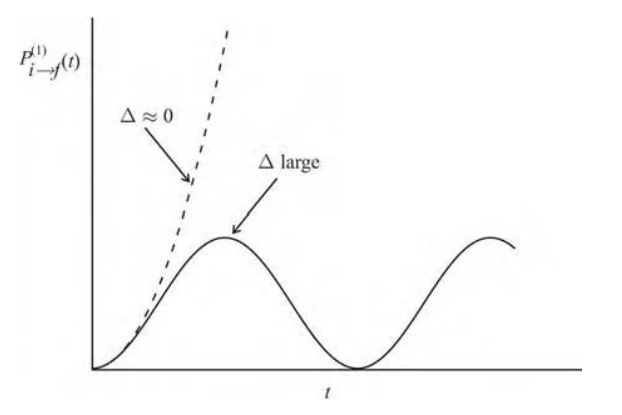
\includegraphics[scale=0.3]{p}
	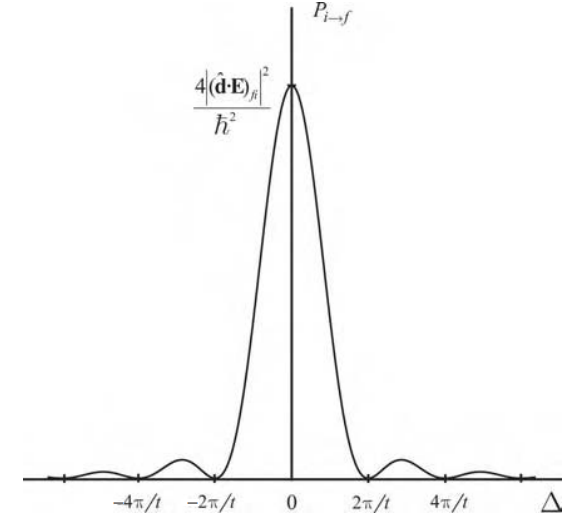
\includegraphics[scale=0.3]{t}
\end{figure}
For the perturbation approximation to be valid we require that $C^{(1)}_f(t) \ll 1$, which implies $P_{i \to f}^{(1)}(t) \ll 1$. For $\Delta \neq 0$, this places constraints on both $\abs{\lp \hat{\mathbf{d}}\cdot\mathbf{E}_0 \rp_{fi}}$ and $\Delta$. On resonance, \eqref{resonance} is only valid for a very short time. For the case of the transition probability as a function of $\Delta$, the width of the peak is proportional to $t^{-1}$ while the height is proportional to $t^2$. It turns out that the area is proportional to $t$:
\begin{align}
\int^{\infty}_{-\infty} \f{\sin^2 \Delta t/2}{\Delta^2} \,d\Delta = \f{\pi t}{2}
\end{align}
In the limit where $\Delta \approx 0$ and $t \gg 2\pi/\omega_{fi}$, the function in the integrand may be approximated by the Dirac delta function
\begin{align}
\lim_{t\to\infty}\f{\sin^2 \Delta t/2}{\Delta^2} = \f{\pi}{2}t\delta(\Delta).
\end{align}
In this case the transition probability is
\begin{align}
P^{(1)}_{i\to f}(t) = \f{\pi}{2}\abs{C^{(1)}_f(t)}^2 = \f{\abs{\lp \hat{\mathbf{d}}\cdot\mathbf{E}_0 \rp_{fi}}^2}{\hbar^2} t \delta(\Delta).
\end{align}
Now we define the time-independent transition probability \textbf{rate} as
\begin{align}
W_{i\to f} = \f{P^{(1)}_{i\to f}}{t} = \f{\pi}{2} \f{\abs{\lp \hat{\mathbf{d}}\cdot\mathbf{E}_0 \rp_{fi}}^2}{\hbar^2} \delta(\omega - \omega_{fi}).
\end{align}
In practice, the driving field will not be monochromatic so that a range of
frequencies will have to be summed or integrated over to obtain the total transition rate.  If $[f]$ represents a set of accessible final states, then the transition rate for a monochromatic field is
\begin{align}
\boxed{W_{i\to [f]} = \f{\pi}{2}\sum_{[f]}\f{\abs{\lp \hat{\mathbf{d}}\cdot\mathbf{E}_0 \rp_{fi}}^2}{\hbar^2} \delta(\omega - \omega_{fi})}
\end{align}
This expression is often famously called Fermi's Golden Rule. Now suppose there is a broad range of frequencies. This means the amplitude of the light is now frequency dependent $\mathbf{E}_0 \to \mathbf{E}_0(\omega)$. Thus the transition probability rate induced by all the frequency components must be
\begin{align}
\f{P^{(1)}_{i\to f}}{t} &=  \int \, d\omega \f{\abs{\lp \hat{\mathbf{d}}\cdot\mathbf{E}_0 \rp_{fi}}^2}{\hbar^2} \f{\sin^2(\Delta t/2)}{\Delta^2}\\
&= \f{1}{\hbar}\int \,d\omega \f{\sin^2(\Delta t/2)}{\Delta^2} \underbrace{\abs{\bra{f}\hat{\mathbf{d}\cdot\mathbf{E}_0(\omega)}\ket{i}}^2}_{F(\omega)}.
\end{align}
Now if $F(\omega)$ varies slowly with $\omega$ compared to $\f{\sin^2(\Delta t/2)}{\Delta^2}$ then we can take $F(\omega)$ to be its resonant value $F(\omega_{fi})$. With this we can take it out of the integral and get
\begin{align}
W_{i\to f} = \f{P^{(1)}_{i\to f}}{t} = \f{\pi}{2\hbar^2}F(\omega_{fi}).
\end{align}
The spread of the frequencies results in the dephasing of the oscillations as shown in the plot of transition probability versus time. This is due to the fact that the light in \textit{incoherent} (lacking the phase relations between the various frequency components). If the atom is driven by coherent light (like a laser), dephasing don't occur and the perturbative time-independent transition rates above generally do not adequately describe the dynamics. We will resolve this issue later. 






 
\subsection{Interaction of an atom with a quantized field \& Spontaneous emission}

In the previous subsection, we did not make any assumption about the relative position of the states $i$ and $f$, i.e., whether $E_i$ is greater or less than $E_f$. We simply said that so long as $\mathbf{E}_0 \neq 0$ and $E_i \neq E_f$, there is some non-zero transition probability. In this section, we will now show that for the case $E_i > E_f$, when the field is quantized, transitions will occur even when no photons are present. This is called \textit{spontaneous emission}. This is one of many differences that appear when we treat the field quantum mechanically versus classically. \\

Let us revisit the single-mode free space field given by \eqref{dipoleE} after dipole approximation (where we assumed the field is uniform over the atom):
\begin{align}
\hat{\mathbf{E}}(\mathbf{r},t)  \approx \hat{\mathbf{E}}(t) = i \lp \f{\hbar\omega_k}{2\epsilon_0 V} \rp^{\f{1}{2}}\mathbf{e} \lb \hat{a}e^{-i\omega t} - \hat{a}^\dagger e^{i\omega t} \rb.
\end{align}
But also recall that this free-space field is written in the Heisenberg picture (there is a time-dependence when the field operator is expressed in the Heisenberg basis). In the Schr\"{o}dinger picture, though, the field operator becomes
\begin{align}
\hat{\mathbf{E}} = i \lp \f{\hbar\omega_k}{2\epsilon_0 V} \rp^{\f{1}{2}}\mathbf{e} \lb \hat{a} - \hat{a}^\dagger \rb.
\end{align}

Now, the free-space Hamiltonian $\hat{\ham}_0$ must be
\begin{align}
\hat{\ham}_0 = \hat{\ham}_\text{atom} + \hat{\ham}_\text{field}
\end{align}
where $\hat{\ham}_\text{atom}$ is just the free-atom Hamiltonian as before and $\hat{\ham}_\text{field}$ is the free-space field Hamiltonian, which we have seen before as well:
\begin{align}
\hat{\ham}_\text{field} = \hbar\omega\lp \hat{a}^\dagger\hat{a} + \f{1}{2} \rp.
\end{align}
Now, because the zero-point energy term does not contribute to the dynamics, we will simply drop it. With this, the interaction Hamiltonian is given by
\begin{align}
\hat{\ham}^{(I)} = -\hat{\mathbf{d}} \cdot\hat{\mathbf{E}} = - i \lp \f{\hbar\omega_k}{2\epsilon_0 V} \rp^{\f{1}{2}}\lp \hat{\mathbf{d}}\cdot\mathbf{e} \rp \lp \hat{a} - \hat{a}^\dagger\rp.
\end{align}
Let us define
\begin{align}
\bm{\mathcal{E}}_0 = i \lp \f{\hbar\omega_k}{2\epsilon_0 V} \rp^{\f{1}{2}}\mathbf{e}.
\end{align}
From this,
\begin{align}
\hat{\ham}^{(I)} = - \hat{\mathbf{d}}\cdot\bm{\mathcal{E}}_0\lp \hat{a} - \hat{a}^\dagger\rp.
\end{align}

Now, because both the atomic and field systems are quantized, the states of the combined system is the product of the states of both the atom and field. Suppose initially we're given the initial state of the atom $\ket{a}$ and $n$ photons $\ket{n}$, then the initial state of the system is
\begin{align}
\ket{i} = \ket{a}\ket{n}. 
\end{align} 
The perturbation interaction of the quantized field causes a transition to the new state 
\begin{align}
\ket{f_1} = \ket{b}\ket{n-1}
\end{align}
where $n-1$ means that one photon has been absorbed by the atom to transition from $\ket{a}$ to $\ket{b}$, or to the state
\begin{align}
\ket{f_2} = \ket{b}\ket{n+1}
\end{align}
where $n+1$ means that one photon has been emitted by the atom to transition from $\ket{a}$ to $\ket{b}$. The energy of these states are
\begin{align}
&\text{for } \ket{i} = \ket{a}\ket{n}, \quad\quad\quad\, E_i = E_a + n\hbar\omega \\
&\text{for } \ket{f_1} = \ket{b}\ket{n-1}, \quad E_i = E_b + (n-1)\hbar\omega \\
&\text{for } \ket{f_2} = \ket{b}\ket{n+1}, \quad E_i = E_b + (n+1)\hbar\omega
\end{align}
where $E_a$ and $E_b$ are the energies of the atomic states $\ket{a}$ and $\ket{b}$. \\

We observe that the interaction Hamiltonian (or the Hamiltonian associated with the perturbation) is time-independent. The matrix elements of this interaction can be calculated by finding
\begin{align}
\text{Absorption: } &\bra{f_1}\hat{\ham}^{(I)}\ket{i}\\
\text{Emission: } &\bra{f_2}\hat{\ham}^{(I)}\ket{i}.
\end{align}
For absorption, we need a term in the interaction Hamiltonian that contains only the annihilation operator:
\begin{align}
\textbf{Absorption: } \bra{f_1}\hat{\ham}^{(I)}\ket{i}
&= \bra{b, n-1}-\hat{\mathbf{d}}\cdot\bm{\mathcal{E}}_0(\hat{a})\ket{a,n}\\
&= \bra{b,n-1}-\hat{\mathbf{d}}\cdot\bm{\mathcal{E}}_0 \sqrt{n}\ket{a,n-1}\\
&= \bra{b}-\hat{\mathbf{d}}\cdot\bm{\mathcal{E}}_0\ket{a}\sqrt{n}\braket{n-1}\\
&= \boxed{-\lp \hat{\mathbf{d}}\cdot\bm{\mathcal{E}}_0 \rp_{ba}\sqrt{n}}
\end{align}
Similarly, for emission
\begin{align}
\textbf{Emission: } \bra{f_2}\hat{\ham}^{(I)}\ket{i}
&= \bra{b, n+1}-\hat{\mathbf{d}}\cdot\bm{\mathcal{E}}_0(-\hat{a}^\dagger)\ket{a,n}\\
&= \bra{b,n+1}\hat{\mathbf{d}}\cdot\bm{\mathcal{E}}_0 \sqrt{n+1}\ket{a,n+1}\\
&= \bra{b}\hat{\mathbf{d}}\cdot\bm{\mathcal{E}}_0\ket{a}\sqrt{n+1}\braket{n+1}\\
&= \boxed{\lp \hat{\mathbf{d}}\cdot\bm{\mathcal{E}}_0 \rp_{ba}\sqrt{n+1}}
\end{align}
where
\begin{align}
\lp \hat{\mathbf{d}}\cdot\bm{\mathcal{E}}_0 \rp_{ba} = \bra{b}\hat{\mathbf{d}}\cdot\bm{\mathcal{E}}_0\ket{a} = \bra{b}\hat{\mathbf{d}}\ket{a}\cdot\bm{\mathcal{E}}_0 \equiv \mathbf{d}_{ba}\cdot\bm{\mathcal{E}}_0
\end{align}
is the dipole matrix element between states $\ket{b}$ and $\ket{a}$. \\

It is worthy to compare this result to the semiclassical picture we saw in the last subsection. For the absorption case, there is nothing new: if no field then no absorption: 
\begin{align}
n=0 \implies \bra{f_1}\hat{\ham}^{(I)}\ket{i} = 0
\end{align}
since $\sqrt{n} = 0$. However, the emission case has no semiclassical counterpart: transitions may occur even when no photons are present:
\begin{align}
n=0 \centernot\implies \bra{f_2}\hat{\ham}^{(I)}\ket{i} = 0
\end{align}
since $\sqrt{n+1}\neq 0$. This is called \textbf{spontaneous emission}, which cannot be obtained from the semiclassical approach. If $n > 0$, the emission of an additional photon is called \textbf{stimulated emission}, which is essential for the operation of the ``light amplification by stimulated emission of radiation'' or LASER. \\

We might also be interested in the ratio of the absorption/emission rates:
\begin{align}\label{rates}
\boxed{\f{\abs{\bra{f_2}\hat{\ham}^{(I)}\ket{i}}^2}{\abs{\bra{f_1}\hat{\ham}^{(I)}\ket{i}}^2}= \f{n+1}{n}}
\end{align}

It turns out that we can still use the perturbation method developed in the previous section to calculate the transition amplitudes, provided that me make appropriate modifications to account for the fact that the field is now quantized. The first difference is in the Hamiltonians:
\begin{align}
\hat{\ham}_0 = \hat{\ham}_\text{atom}  &\to \hat{\ham}_0 =  \hat{\ham}_\text{atom} + \hat{\ham}_\text{field}\\
\hat{\ham}^{(I)}(t) = -\hat{\mathbf{d}}\cdot\mathbf{E}(t) &\to \hat{\ham}^{(I)}(t) = - \hat{\mathbf{d}}\cdot\bm{\mathcal{E}}_0\lp \hat{a} - \hat{a}^\dagger\rp
\end{align}
where of course
\begin{align}
\hat{\ham}_\text{field} = \hbar\omega\lp \hat{a}^\dagger\hat{a} + \f{1}{2} \rp
\end{align}
where we again leave out the zero-point energy term. \\

Now, let us assume that the atom has only two levels $\ket{a}$ and $\ket{b}$. The state vector of the system can be written as
\begin{align}
\ket{\psi(t)} = &C_i(t)\ket{a}\ket{n}e^{-i\omega_a t}e^{-i n \omega t } \nonumber\\
&+ C_{f_1}(t)\ket{b}\ket{n-1}e^{-i\omega_b t}e^{-i (n-1) \omega t } \nonumber\\
&+ C_{f_2}(t)\ket{b}\ket{n+1}e^{-i\omega_b t}e^{-i (n+1) \omega t } 
\end{align}
where the first term is the initial state of the system, the second term is corresponds to absorption, and the third term corresponds to emission. We assume that $\ket{\psi(t)} = \ket{a}\ket{n}$, $C_i(0) = 1$, and $C_{f_1}(0) = C_{f_2}(0) = 0$. Following the perturbative method used before, we can get the first-order correction
for the amplitudes $C_{f_1}$ and $C_{f_2}$ associated with the atom being in state $\ket{b}$:
\begin{align}
\text{Absorption: }&C_{f_1}^{(1)}(t) = -\f{i}{\hbar}\int_0^t \,dt' \bra{f_1}\hat{\ham}^{(I)}\ket{i}e^{i(\omega_{f_1} - \omega_i)t'}\\
\text{Emission: }&C_{f_2}^{(1)}(t) = -\f{i}{\hbar}\int_0^t \,dt' \bra{f_2}\hat{\ham}^{(I)}\ket{i}e^{i(\omega_{f_2} - \omega_i)t'}.
\end{align}
And so the amplitude of the atom being in state $\ket{b}$ (to first-order of course) regardless of how it got there is the \textit{sum} of these amplitudes:
\begin{align}\label{quantum_amp}
C_f^{(1)}(t) &= C_{f_1}^{(1)}(t) + C_{f_2}^{(1)}(t)\\
&= \f{i}{\hbar}\lp \hat{\mathbf{d}}\cdot\bm{\mathcal{E}}_0 \rp_{ba}\int^t_0 \,dt'  \sqrt{n}  e^{i(\omega_{f_1} - \omega_i)t'} 
- \sqrt{n+1}  e^{i(\omega_{f_2} - \omega_i)t'}\\
&= \boxed{\f{i}{\hbar}\lp \hat{\mathbf{d}}\cdot\bm{\mathcal{E}}_0 \rp_{ba}
\lb \underbrace{\sqrt{n+1}\cdot\f{e^{i(\omega + \omega_{ba})t} - 1}{ \omega + \omega_{ba} }}_\text{Emission}  - \underbrace{\sqrt{n}\cdot\f{e^{i(\omega - \omega_{ba})t} - 1}{\omega - \omega_{ba}}}_{\text{Absorption}}\rb}
\end{align}
If $n\ll 1$ then $\sqrt{n+1} \approx \sqrt{n}$, in which case this result and \eqref{amplitude} are essentially the same and we get a correspondence between classical and quantum field amplitudes:
\begin{align}
\lp \mathbf{E}_0 \rp_\text{classical} \leftrightarrow \lp 2i\mathcal{E}_0\sqrt{n} \rp_\text{quantum}.
\end{align}

If $E_b > E_a$ ($\ket{b}$ is the excited state) and $\omega \approx \omega_{ba}$ then by RWA the first term in \eqref{quantum_amp} can be dropped as the second term dominates. There is nothing abnormal about this. However, if $E_a > E_b$ ($\ket{a}$ is the excited state) and $\omega \approx -\omega_{ba}$, then the second term of \eqref{quantum_amp} can be dropped (again under RWA). This leaves us with
\begin{align}
C_f^{(1)}(t) \approx \f{i}{\hbar}\lp \hat{\mathbf{d}}\cdot\bm{\mathcal{E}}_0 \rp_{ba}
\lb \underbrace{\sqrt{n+1}\cdot\f{e^{i(\omega + \omega_{ba})t} - 1}{ \omega + \omega_{ba} }}_\text{Emission}\rb.
\end{align}
We notice that even when $n=0$, this does not vanish. In this case, the transition between $\ket{a}$ and $\ket{b}$ occurs through spontaneous emission. 




\subsubsection{Field-theoretic derivation of the Planck's distribution}

Suppose we have a collection of atoms interacting resonantly with a quantized field of frequency
\begin{align}
\omega = \f{E_a - E_b}{\hbar}
\end{align}
where $\ket{a}$ and $\ket{b}$ are atomic eigenstates with $E_a > E_b$. Let $N_a, N_b$ be the populations of atoms in $\ket{a}$ and $\ket{b}$ respectively. Let $W_\text{emis}$ and $W_\text{abs}$ be the transition rate due to photon emission and absorption respectively. We have the following set of differential equations:
\begin{align}
&\f{dN_a}{dt} = -N_a W_\text{emis} + N_b W_\text{abs}\\
&\f{dN_b}{dt} = -N_b W_\text{abs} + N_a W_\text{emis}.
\end{align}
At thermal equilibrium:
\begin{align}
\f{dN_a}{dt} = 0 = \f{dN_b}{dt} \implies N_a W_\text{emis} = N_b W_\text{abs}.
\end{align}
From the relative rates in \eqref{rates}, we have
\begin{align}\label{1}
\f{N_b}{N_a} = \f{W_\text{emis}}{W_\text{abs}} = \f{n+1}{n}.
\end{align}
Now, according to Boltzmann statistics:
\begin{align}\label{2}
\f{N_b}{N_a} = e^{(E_a - E_b)/kT} = e^{\hbar\omega /kT}. 
\end{align}
From \eqref{1} and \eqref{2} we have
\begin{align}
\boxed{n = \f{1}{e^{\hbar\omega/kT} - 1}}
\end{align}

There's a slightly different derivation by Einstein (which was done even before quantum electrodynamics was invented), which takes into account as well the distinction between spontaneous and stimulated emission. We won't go into the details of this. 



\subsection{The Rabi model}

In the previous subsections we have used the perturbation theory approach to calculate transition probabilities. This approach assumes that the population in the initial state is essentially unchanged and the population in the final states are very small. This approach fails in cases of large population transfer, for example when there is a strong, near resonance (with one state and no other) laser field. In this case, the perturbation approach must be abandoned, only two dominant states remain, and the problem can solved ``exactly.'' This is the \textbf{Rabi model}. We note that the Rabi model is a \textit{semiclassical model}. The full quantum mechanical model is covered in the next subsection. \\

Suppose our two levels are the ground $\ket{g}$ and excited state $\ket{e}$. The transition frequency is given by
\begin{align}
\omega_0 = \f{E_e - E_g}{\hbar} \approx \omega
\end{align}
where $\omega$ is the frequency of the driving field. Once again, the interaction Hamiltonian is given by
\begin{align}
\hat{\ham}^{(I)} = -\hat{\mathbf{d}}\cdot\mathbf{E}_0 \cos\omega t \equiv \hat{V}_0 \cos\omega t
\end{align}
where again the dipole approximation is already made. The state vector is a linear combination of the eigenstates:
\begin{align}
\ket{\psi(t)} = C_g(t)e^{-iE_gt/\hbar}\ket{g} + C_e(t)e^{-iE_et/\hbar}\ket{e}.
\end{align}
The Schr\"{o}dinger equation
\begin{align}
i\hbar \f{\p \ket{\psi(t)}}{\p t} &= \lp \hat{\ham}_0 + \hat{\ham}^{(I)} \rp \ket{\psi(t)}\\
&=\lp \hat{\ham}_0 + \hat{V}_0 \cos\omega t \rp \ket{\psi(t)}
\end{align}
gives a system of differential equations:
\begin{align}
\begin{bmatrix}
\dot{C}_g \\ \dot{C}_e
\end{bmatrix}
=
\begin{bmatrix}
0 &-\f{i}{\hbar}\bra{g}\hat{V}_0 \ket{e}e^{-i\omega_0 t} \\ 
-\f{i}{\hbar}\bra{g}\hat{V}_0 \ket{e}e^{i\omega_0 t} & 0
\end{bmatrix}
\begin{bmatrix}
C_g \\ C_e
\end{bmatrix}
\end{align}
where the first equation is obtained by multiplying the SE from the left by $e^{i\omega_g t}\bra{g}$ and the fact that $\bra{i}\hat{V}_0\ket{j} = 0$ when $i = j$. Next, we assume that $\bra{g}\hat{V}_0 \ket{e}$ is real and $C_g(0) = 1, C_e(0) = 0$. Let us call
\begin{align}
\mathcal{V} = \bra{g}\hat{V}_0 \ket{e}
\end{align}
and approximate $\cos\omega t$ in exponentials and keep only the terms that oscillate at frequency $\omega - \omega_0$ to get
\begin{align}
&\dot{C}_g = -\f{i}{2\hbar}\mathcal{V}e^{i(\omega - \omega_0 )t}C_e\\
&\dot{C}_e = -\f{i}{2\hbar}\mathcal{V}e^{-i(\omega - \omega_0 )t}C_g.
\end{align}
Taking the derivative of the second equation, plugging it into the first while applying RWA (eliminating terms with $\omega + \omega_0$) we get
\begin{align}
\ddot{C}_e + i(\omega - \omega_0 )\dot{C}_e + \f{1}{4}\f{\mathcal{V}^2}{\hbar^2}C_e = 0.
\end{align}
This differential equation is quite a classic. The general solution is
\begin{align}
C_e(t) = A_+ e^{i\lambda_+ t} + A_- e^{i\lambda_- t} 
\end{align}
where with $\Delta = \omega - \omega_0$,
\begin{align}
\lambda_{\pm} = \f{1}{2}\lb \Delta \pm \sqrt{ \Delta^2 + \f{\mathcal{V}^2}{\hbar^2}} \rb.
\end{align}
From the initial conditions, we also have that
\begin{align}
A_{\pm} = \mp \f{1}{2\hbar}\f{\mathcal{V}}{\sqrt{\Delta^2 + \f{\mathcal{V}^2}{\hbar^2}}}.
\end{align}
With this, the solution to the problem is
\begin{align}
&C_e(t) = i\f{\mathcal{V}}{\Omega_R \hbar}e^{i\Delta t/2}\sin\f{\Omega_R t}{2}\\
&C_g(t) = e^{i\Delta t/2} \lc \cos\f{\Omega_R t}{2} - i\f{\Delta}{\Omega_R}\sin\f{\Omega_R t}{2} \rc
\end{align}
where
\begin{align}
\Omega_R = \sqrt{\Delta^2 + \f{\mathcal{V}^2}{\hbar^2}}
\end{align}
is called the \textbf{Rabi frequency}, or \textbf{Rabi rate}. \\

The probability that the atom is in the excited state $\ket{e}$ is then
\begin{align}
\boxed{P_e(t) = \abs{C_e(t)}^2 = \f{\mathcal{V}^2}{\Omega_R^2\hbar^2}\sin^2\f{\Omega_R t}{2}}
\end{align}
On resonance, this probability is a perfect sine-squared:
\begin{align}
\boxed{P_e(t) = \sin^2\f{\mathcal{V}t}{2\hbar}}
\end{align}
where at $t= \pi \hbar / \mathcal{V}$ all the atomic population is transferred to the excited state. The following plot illustrates the population transfer and ``oscillation''
\begin{figure}[!htb]
	\centering
	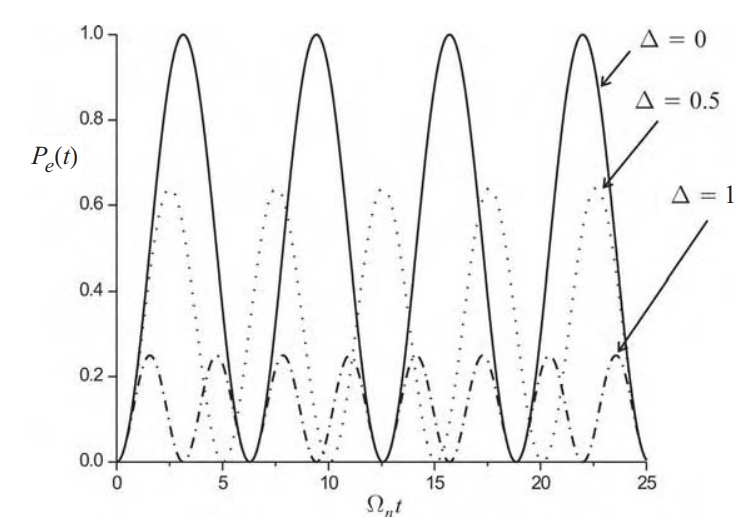
\includegraphics[scale=0.3]{rabi}
\end{figure}

The \textbf{atomic inversion} $W(t)$ is defined as the difference in population between the excited and ground states:
\begin{align}
W(t) = P_e(t) - P_g(t).
\end{align}
For the case of resonance ($\Delta = 0$) and that initially the atom is in the ground state, 
\begin{align}
W(t) = \sin^2 \f{\mathcal{V}t}{2\hbar} - \cos^2 \f{\mathcal{V}t}{2\hbar} = -\cos\f{\mathcal{V}t}{\hbar} = -\cos\Omega_R(\Delta = 0)t.
\end{align}
For $t = \pi\hbar/\mathcal{V}$, $W(\pi\hbar/\mathcal{V}) = 1$. This kind of population transfer is called the $\pi-$pulse. For $t = \pi\hbar/2\mathcal{V}$, $W(\pi\hbar/2\mathcal{V}) = 0$, which means the population is shared coherently between the ground and excited states, i.e., the system is in a perfect superposition:
\begin{align}
\ket{\psi(t)} = \f{1}{\sqrt{2}}\lp\ket{g} + i\ket{e} \rp.
\end{align}










\subsection{Fully quantum-mechanical model; the Jaynes–Cummings model}

We move on to the quantum electrodynamics version of the Rabi model. In our previous discussion of the interaction between atoms and the quantized field, we assumed the field is single-mode. We again assume this, such that the single-mode cavity field can be written as
\begin{align}
\mathbf{\hat{E}} = \mathbf{e}\lp \f{\hbar\omega}{\epsilon_0 V} \rp^{1/2}\lp \hat{a} + \hat{a}^\dagger\rp\sin(kz)
\end{align}
where $\mathbf{e}$ is some arbitrary polarization vector. We also assume that the atom has two levels $\ket{g}$ and $\ket{e}$. The interaction Hamiltonian is given by
\begin{align}
\hat{\ham}^{(I)} = -\mathbf{\hat{d}} \cdot \mathbf{\hat{E}} = \hat{d} g (\hat{a} + \hat{a}^\dagger)
\end{align}
where
\begin{align}
\hat{d} &= \mathbf{d} \cdot \mathbf{e}\\
g &=  \lp \f{\hbar\omega}{\epsilon_0 V} \rp^{1/2}\sin(kz).
\end{align}

For simplicity, let us introduce the atomic transition operators 
\begin{align}
\text{Excitation: } &\hat{\sigma}_+ = \ket{e}\bra{g}\\
\text{De-excitation: } &\hat{\sigma}_- = \ket{g}\bra{e} = \hat{\sigma}_+^\dagger.
\end{align}
The inversion operator is given by
\begin{align}
\hat{\sigma}_3 = \ket{e}\bra{e} - \ket{g}\bra{g}.
\end{align}
We can verify that these operators obey the Pauli spin algebra:
\begin{align}
[\hat{\sigma}_+, \hat{\sigma}_-] &= \hat{\sigma}_3\\
[\hat{\sigma}_3, \hat{\sigma}_\pm] &= 2\hat{\sigma}_\pm.
\end{align}

We know that the diagonal matrix elements of $\hat{d}$ is zero because $\bra{e}\hat{d}\ket{e} = \bra{g}\hat{d}\ket{g} = 0$. This means with $d = \bra{e}\hat{d}\ket{g}$, we can write in the basis
\begin{align}
\hat{d} &= d\ket{g}\bra{e} + d^*\ket{e}\bra{g}\\
&= d\hat{\sigma}_- + d^*\hat{\sigma}_+\\
&= d\lp \hat{\sigma}_- + \hat{\sigma}_+ \rp.
\end{align}
This gives the interaction Hamiltonian:
\begin{align}
\hat{\ham}^{(I)} = \hbar \lp \f{dg}{\hbar} \rp \lp \hat{\sigma}_- + \hat{\sigma}_+ \rp \lp \hat{a} + \hat{a}^\dagger \rp. 
\end{align}
Define the energy to be zero halfway between the states, then we have $E_e = -E_g$, and the free atomic Hamiltonian can be written as
\begin{align}
\hat{\ham}_0 = \f{\hbar}{2}\begin{bmatrix}
E_e & \\ & E_g
\end{bmatrix} 
\end{align}
or in the basis
\begin{align}
\hat{\ham}_0 = \f{1}{2}\hbar\omega_0 \lp \ket{e}\bra{e} - \ket{g}\bra{g} \rp = \f{1}{2}\hbar\omega_0 \hat{\sigma}_3 
\end{align}
where 
\begin{align}
E_e = -E_g = \f{1}{2}\hbar\omega_0
\end{align}
and of course $\omega_0$ is the transition frequency. The free-field Hamiltonian after dropping the zero-point energy term, again, is
\begin{align}
\hat{\ham}_F = \hbar\omega\hat{a}^\dagger\hat{a}.
\end{align}
So the total Hamiltonian is
\begin{align}
\hat{\ham} &= \hat{\ham}_0 + \hat{\ham}_F + \hat{\ham}^{(I)}\\
&= \f{1}{2}\hbar\omega_0 \hat{\sigma}_3  + \hbar\omega\hat{a}^\dagger\hat{a} + \hbar \lp \f{dg}{\hbar} \rp \lp \hat{\sigma}_- + \hat{\sigma}_+ \rp \lp \hat{a} + \hat{a}^\dagger \rp.
\end{align}
Let us call
\begin{align}
\lambda = \f{dg}{h}.
\end{align}
It follows that
\begin{align}
\hat{\ham} = \f{1}{2}\hbar\omega_0 \hat{\sigma}_3  + \hbar\omega\hat{a}^\dagger\hat{a} + \hbar \lambda\lp  \hat{\sigma}_- + \hat{\sigma}_+ \rp \lp \hat{a} + \hat{a}^\dagger \rp.
\end{align}
Let us simplify this Hamiltonian with some approximations. We know that in the field-free case, the creation and annihilation operators evolve in time as
\begin{align}
\hat{a}(t) = \hat{a}(0)e^{-i\omega t} \hspace{0.5cm} \hat{a}^\dagger(t) = \hat{a}^\dagger(0)e^{i\omega t},
\end{align}
while in the free atomic case the excitation operators (which we can show) to evolve in time as
\begin{align}
\hat{\sigma}_{\pm}(t) = \hat{\sigma}_\pm(0)e^{\pm i \omega_0 t}.
\end{align}
This gives us some idea of the time dependency of the product of some of these operators:
\begin{align}
&\hat{\sigma}_+ \hat{a} \sim e^{i(\omega_0 - \omega)t}\\
&\hat{\sigma}_- \hat{a}^\dagger \sim e^{-i(\omega_0 - \omega)t}\\
&\hat{\sigma}_+ \hat{a}^\dagger \sim e^{i(\omega_0 + \omega)t}\\
&\hat{\sigma}_- \hat{a} \sim e^{-i(\omega_0 + \omega)t}.
\end{align}
For $\omega_0 \approx \omega$ we can use RWA to ignore the last two terms. The term $\hat{\sigma}_+ \hat{a}^\dagger$ corresponds to the emission of a photon (the creation operator) as the atom goes from the ground to the excited state, while the term $\hat{\sigma}_- \hat{a}$ corresponds to the absorption of a photon (the annihilation operator) as the atom goes from the excited to ground state. It makes good sense to ignore these terms, so that we're left with the approximate Hamiltonian:
\begin{align}
\boxed{\hat{\ham} = \f{1}{2}\hbar\omega_0 \hat{\sigma}_3  + \hbar\omega\hat{a}^\dagger\hat{a} + \hbar \lambda\lp  \hat{\sigma}_+ \hat{a}  + \hat{\sigma}_-\hat{a}^\dagger \rp}
\end{align}
This is called the \textbf{Jaynes-Cummings model}. To solve the dynamics of the system, we first note a few constants. The first constants is the number of electrons, or the total probability of the atom being in either state $\ket{e}$ or $\ket{g}$:
\begin{align}
\hat{P}_E = \ket{e}\bra{e} + \ket{g}\bra{g} = 1.
\end{align}
and of course this quantity is conserved: 
\begin{align}
[\hat{\ham}, \hat{P}_E] \propto \f{d\hat{P}_E}{d t} = 0.
\end{align}
The excitation number is also unchanged: 
\begin{align}
\hat{N}_e = \hat{a}^\dagger\hat{a} + \ket{e}\bra{e} \implies [\hat{\ham}, \hat{N}_e] \propto \f{d\hat{N}_e}{dt} = 0.
\end{align}
This equation essentially says the number of electrons created corresponds to the transitions.\\

With these constants we may break the Hamiltonian into two commuting parts:
\begin{align}
\hat{\ham} = \hat{\ham}_I + \hat{\ham}_{II}
\end{align}
where
\begin{align}
\hat{\ham}_I &= \hbar\omega \hat{N}_e + \hbar\lp \f{\omega_0}{2} - \omega \rp\hat{P}_E\\
\hat{\ham}_{II} &= -\hbar\Delta + \hbar \lambda \lp \hat{\sigma}_+ \hat{a}  + \hat{\sigma}_-\hat{a}^\dagger \rp
\end{align}
All dynamics is contained in $\hat{H}_{II}$, while $\hat{\ham}_I$ contributes to (irrelevant) phase factors. Next, let us examine a few notable cases. 

\subsubsection{Resonance: $\Delta = 0$}

Let us assume that initially the atom is in the excited state $\ket{e}$ and the field is initially in the state $\ket{n}$. The initial atom-field state is
\begin{align}
\ket{i} = \ket{e}\ket{n}.
\end{align}
The energy of this state is of course
\begin{align}
E_i  = E_e + E_n = \f{1}{2}\hbar\omega + n\hbar\omega
\end{align}
where recall that we have set zero energy to be in the middle of the two states. This initial state $\ket{i}$ to coupled to and only to the final state $\ket{f} = \ket{g}\ket{n+1}$. The state vector is given by
\begin{align}
\ket{\psi(t)} = C_i(t) \ket{i} + C_f(t)\ket{f}
\end{align}
with $C_i(0) = 1$ and $C_f(0) = 0$. In the interaction picture, 
\begin{align}
i\hbar \f{d\ket{\psi(t)}}{dt} = \hat{\ham}_{II}\ket{\psi(t)}.
\end{align}
Plugging $\hat{\ham}_{II}$ in and solve we obtain
\begin{align}
\dot{C}_i &= -i\lambda \sqrt{n+1}C_f\\
\dot{C}_f &= -i\lambda \sqrt{n+1}C_i. 
\end{align}
By eliminating $C_f$ and solving, we get 
\begin{align}
C_i(t) = \cos\lp  \lambda t \sqrt{n+1} \rp
\end{align}
and 
\begin{align}
C_f(t) =-i\sin\lp \lambda t \sqrt{n+1} \rp.
\end{align}
With this, the probability that the system is in the initial state is
\begin{align}
P_i(t) = C_i^*(t)C_i(t) = \cos^2 \lp  \lambda t \sqrt{n+1} \rp.
\end{align}
And the probability that the system is in the other state is of course
\begin{align}
P_f(t) = \sin^2\lp  \lambda t \sqrt{n+1} \rp.
\end{align}
The atom inversion is then
\begin{align}
W(t) = P_i(t) - P_f(t) = \cos\lp 2\lambda t \sqrt{n+1} \rp.
\end{align}
We may define a quantum electrodynamic Rabi frequency
\begin{align}
\boxed{\Omega(n) = 2\lambda\sqrt{n+1}}
\end{align}
This gives
\begin{align}
W(t) = \cos\lp \Omega(n)t \rp.
\end{align}
We notice that there's Rabi oscillation, which we also see in the classical case. However, there is still Rabi oscillation in the case of $n=0$. These is vacuum Rabi oscillation. They are the result of the atom spontaneously emitting a photon then re-absorbing it, re-emitting it, etc.: an example of reversible spontaneous emission.


\subsubsection{Pure state}
In this scenario we assume that the atom is initially in a superposition of $\ket{e}$ and $\ket{g}$. 
\begin{align}
\ket{\psi(t)}_\text{atom} =C_e\ket{e} + C_g\ket{g}.
\end{align}
The field is initially in the state
\begin{align}
\ket{\psi(t)}_\text{field} = \sum_{n=0}^\infty C_n\ket{n}.
\end{align}
Thus the initial state of the system is given by a tensor product
\begin{align}
\ket{\psi(t)} = \ket{\psi(0)}_\text{atom} \otimes \ket{\psi(0)}_\text{field}.
\end{align}
The solution to the Schr\"{o}dinger equation is now
\begin{align}
\ket{\psi(t)} = \sum^\infty_{n=0}\lc \lb C_e C_n \cos (\lambda t \sqrt{n+1}) - iC_gC_{n+1}\sin(\lambda t \sqrt{n+1}) \rb \ket{e} \right. \nonumber \\  \left.
+ \lb -iC_eC_{n-1}\sin(\lambda t \sqrt{n}) + C_gC_n \cos(\lambda t \sqrt{n}) \rb 
 \rc \otimes \ket{n}.
\end{align}
This is an entangled state. Now, if $C_e = 1$ and $C_g = 0$ initially, then
\begin{align}
\ket{\psi(t)} = \ket{\psi_g(t)}\otimes \ket{g} + \ket{\psi_e(t)}\otimes \ket{e},
\end{align}
where
\begin{align}
&\ket{\psi_g(t)} = -i\sum^\infty_{n=0}C_n\sin(\lambda t \sqrt{n+1})\ket{n+1}\\
&\ket{\psi_e(t)} = \sum^\infty_{n=0}C_n\cos(\lambda t \sqrt{n+1})\ket{n}.
\end{align}
The atomic inversion is then
\begin{align}
W(t) &= \bra{\psi(t)}\hat{\sigma}_3\ket{\psi(t)}\\
&= \braket{\psi_e(t)} - \braket{\psi_g(t)}\\
&= \sum^\infty_{n=0}\abs{C_n}^2 \cos(2\lambda t\sqrt{n+1}).
\end{align}


\subsection{The Density Operator approach (or the master equation's approach) }
So far, we have considered only cases where the field and the atom are initially in pure states. The density operator approach allows us to solve for a more general case. Let us work in the interaction picture again where the interaction Hamiltonian is given by
\begin{align}
\hat{\ham}_I = \hbar\lambda \lp \hat{a}\hat{\sigma}_+ + \hat{a}^\dagger\hat{\sigma}_- \rp
\end{align}
Let us consider the density operator of the atom-field system at time $t$. As we know the density operator is defined to be
\begin{align}
\hat{\rho} = \ket{\psi}\bra{\psi}.
\end{align}
Applying the Schr\"{o}dinger equation to $\ket{\psi}$, we have
\begin{align}
i\hbar \f{d\ket{\psi}}{dt} = \hat{\ham}_I \ket{\psi}.
\end{align}
Now let us see what we get when we look at the time evolution of the density operator
\begin{align}
\f{d \hat{\rho}}{dt} &= \f{d\ket{\psi}}{dt} \bra{\psi} + \ket{\psi}\f{d\bra{\psi}}{dt}\\
&= \lb \f{-i}{\hbar}\hat{\ham}_I\ket{\psi} \rb\bra{\psi} + \ket{\psi}\lb \f{i}{\hbar}\bra{\psi} \hat{\ham}_I \rb\\
&= \f{-i}{\hbar}\lb \hat{\ham}_I\ket{\psi}\bra{\psi} - \ket{\psi}\bra{\psi}\hat{\ham}_I \rb\\
&= \f{-i}{\hbar}\lb \hat{\ham}_I, \hat{\rho} \rb.
\end{align}
The solution to this (which we can quite easily verify) is 
\begin{align}\label{rho}
\hat{\rho}(t) = e^{-i\hat{\ham}_I t/\hbar}\hat{\rho}(0)e^{i\hat{\ham}_I t/\hbar} = \hat{U}_I(t)\hat{\rho}(0)\hat{U}_I^\dagger(t).
\end{align} 
Recall that the Hamiltonian can be expressed further in terms of the excitation/de-excitation, and inversion operators, whose matrix representations are
\begin{align}
\sigma_+ = \begin{bmatrix}
0 & 1\\0 & 0
\end{bmatrix}, \hspace{0.5cm}
\sigma_- = \begin{bmatrix}
0 & 0 \\ 1 & 0
\end{bmatrix}, \hspace{0.5cm}
\sigma_3 = \begin{bmatrix}
1 & 0 \\ 0 & -1
\end{bmatrix}
\end{align}
where we have used the convention
\begin{align}
\sigma_j = \begin{bmatrix}
\bra{e}\hat{\sigma}_j\ket{e} & \bra{e}\hat{\sigma}_j\ket{g}\\
\bra{g}\hat{\sigma}_j\ket{e} &
\bra{g}\hat{\sigma}_j\ket{g} 
\end{bmatrix}, \hspace{0.5cm} j = \pm, 3.
\end{align}
Let us re-write $\hat{U}_I(t)$ in terms of these operators:
\begin{align}
\hat{U}_I(t) = e^{-i\hat{H}_I t/\hbar} = e^{-i\lambda t (\hat{a}\hat{\sigma}_+ + \hat{a}^\dagger\hat{\sigma_-})}.
\end{align}
With this, we can write the evolution operator $\hat{U}_I$ in terms of cosines and sines as
\begin{align}
\hat{U}_I(t) = \begin{bmatrix}
\hat{C}(t) & \hat{S}'(t) \\ \hat{S}(t) & \hat{C}'(t)
\end{bmatrix}
\end{align}
where
\begin{align}
&\hat{C}(t) = \cos(\lambda t \sqrt{\hat{a}\hat{a}^\dagger})\\
&\hat{S}(t) = -i\hat{a}^\dagger\f{\sin(\lambda t \sqrt{\hat{a}\hat{a}^\dagger})}{\sqrt{\hat{a}\hat{a}^\dagger}}\\
&\hat{C}'(t) = \cos(\lambda t \sqrt{\hat{a}^\dagger\hat{a}})\\
&\hat{S}'(t) =  -i\hat{a}\f{\sin(\lambda t \sqrt{\hat{a}^\dagger\hat{a}})}{\sqrt{\hat{a}^\dagger\hat{a}}}.
\end{align}
It is then easy to show that
\begin{align}
\hat{U}^\dagger_I(t) = \hat{U}_I(-t) = \begin{bmatrix}
\hat{C}(t) & -\hat{S}'(t) \\ -\hat{S}(t) & \hat{C}'(t)
\end{bmatrix}.
\end{align}
Now, suppose at $t=0$ the density operator for the atom-field system can be written as a tensor product of the field and atom parts (not entangled):
\begin{align}
\hat{\rho}(0) = \hat{\rho}^F(0)\otimes \hat{\rho}^A(0).
\end{align}
Next, suppose that our atom is initially in $\ket{e}$, such that by convention the atom's density matrix is
\begin{align}
\rho^A(0) = \begin{bmatrix}
1 & 0 \\ 0 & 0
\end{bmatrix}.
\end{align}
Thus for the system,
\begin{align}
\hat{\rho}(0) = \hat{\rho}^F(0) \otimes \begin{bmatrix}
1 & 0 \\ 0 & 0
\end{bmatrix} = \begin{bmatrix}
\hat{\rho}^F(0) & 0 \\ 0 & 0 
\end{bmatrix}.
\end{align}
Now by \eqref{rho},
\begin{align}
\hat{\rho}(t) = \begin{bmatrix}
\hat{C}(t)\hat{\rho}^F(0)\hat{C}(t) & -\hat{C}(t)\hat{\rho}^F(0)\hat{S}'(t)\\
\hat{S}(t)\hat{\rho}^F(0)\hat{C}(t) & -\hat{S}(t)\hat{\rho}^F(0)\hat{S}'(t)
\end{bmatrix}.
\end{align}

To find the density operator of the field, we trace over the atomic states:
\begin{align}
\hat{\rho}^F(t) = \Tr_A \hat{\rho}(t) = \hat{C}(t)\hat{\rho}^F(0)\hat{C}(t) -\hat{S}(t)\hat{\rho}^F(0)\hat{S}'(t).
\end{align}
The matrix elements for the field are then
\begin{align}
\hat{\rho}^F_{nm} &\equiv \bra{n}\hat{\rho}^F(t)\ket{m} \\ 
&= \bra{n} \hat{C}(t)\hat{\rho}^F(0)\hat{C}(t) \ket{m} - \bra{n} \hat{S}(t)\hat{\rho}^F(0)\hat{S}'(t) \ket{m}.
\end{align}
On the other hand, tracing over the field states (there are infinitely many) we obtain the density operator of the atom:
\begin{align}
\hat{\rho}^A(t) = \Tr_F \hat{\rho}(t) = \sum^\infty_{n=0} \bra{n}\hat{\rho}(t)\ket{n}.
\end{align}
The matrix elements are then
\begin{align}
\bra{i}\hat{\rho}^A(t)\ket{j} = \sum^\infty_{n=0}\bra{i,n} \hat{\rho}_F(t)\ket{j,n}
\end{align}
where $i,j = e,g$. The diagonal elements $\rho^A_{ee}$ and $\rho^A_{gg}$ are the populations of the excited and ground states and satisfy
\begin{align}
\rho^A_{gg}(t) + \rho^A_{ee}(t) = 1
\end{align}
for any time $t$. The atomic inversion is
\begin{align}
W(t) = \rho^A_{ee}(t) - \rho^A_{gg}(t) = 2\rho^A_{ee}(t) - 1.
\end{align}
We can find that
\begin{align}
\rho^A_{ee}(t) &= \sum^\infty_{n=0}\bra{n}\hat{C}(t)\hat{\rho}^F(0)\hat{C}(t)\ket{n}\\
&= \sum^\infty_{n=0}\bra{n}\hat{\rho}^F(0)\ket{n}\cos^2(\lambda t \sqrt{n+1}).
\end{align}
\subsubsection{Pure state}
If the field is initially in a pure state
\begin{align}
\ket{\psi_F(0)} = \sum^\infty_{n=0}C_n\ket{n},
\end{align}
then
\begin{align}
\hat{\rho}^F(0) = \ket{\psi_F}\bra{\psi_F},
\end{align}
which gives
\begin{align}
\rho^A_{ee}(t) = \sum^\infty_{n=0}\abs{C_n}^2\cos^2(\lambda t \sqrt{n+1}).
\end{align}
This gives the atomic inversion we have found before. 
\subsubsection{Mixed state}
However, if the field is initially in a thermal state (mixed state) where
\begin{align}
\hat{\rho}^F(0) = \hat{\rho}_{Th} = \sum P_n\ket{n}\bra{n}
\end{align}
where $P_n$ is probability. The atomic inversion in this case is
\begin{align}
W(t) = \sum^\infty_{n=0}P_n \cos(2\lambda t\sqrt{n+1}),
\end{align}
which is slightly different. 



















\newpage

\section{Collective Atomic Interactions}



\newpage


\chapter{QUANTUM INFORMATION}















\chapter{PROBLEMS \& SOLUTIONS}

\newpage

\section{Quantum Mechanics}

\newpage

\section{Quantum Optics}

\newpage

\section{Quantum Information}



\newpage

% move this somewhere else later

One photon, two photons, red photon, blue photon.\\
JQI Summer School\\
Elizabeth Goldschmidt\\
July 19, 2019\\

Topic: single photon, single photon statistics. \\

\textbf{Why?}
\begin{itemize}
	\item Why single photons?
	\item Why is it hard?
\end{itemize}


\textbf{Sending QI}
\begin{itemize}
	\item Sending quantum information as light (not as easy any other way)
	\item requires encoding qubits in light
	\item qubits must be identical in all other degrees of freedom: polarizations, transverse/longitudinal modes....
	\item How else can you do it LOL?
\end{itemize}


\textbf{Single photon: } single excitation of a single mode of the quantized EM field. This treats photon number differently from other dfs. There's a fundametal difference between 0 and multiple excitations. 

\textbf{Photon number:}
\begin{itemize}
	\item Classical light: spectral and photon number distribution depend on system (source). 
	\item Why can't I turn down intensity to get single photon? Because probability of getting 2 saturates.
	\item Photon number is not a good quantum number.
	\item So what do we do? $\implies$ reduce variance.
	\item How to quantify? Use $g^{(2)}$ - autocorrelation function. For weak fields
	\begin{align}
	g^{(2)} = \f{conincidence}{individual\times individual} \approx = \f{2 p(2)}{p(1)^2}
	\end{align}
	independent of attenuation.
	\item \textbf{Cauchy-Schwarz}. Classically, operators commute... 
	such that $g^{(2)} \geq 1$ (no anti-bunching light). But because of QM, $g^{(2)}$ can be less than 1. 
\end{itemize}


\textbf{Other dfs: } the well-defined single mode covers all the other degrees of freedom (spatial, spectral, temporal, polarization, etc.) How to quantify single-photon? $\implies$ Two-photon (Hong-Ou-Mandel) Interference. 
\begin{itemize}
	\item Measure indistinguishability to characterize single photons. 
\end{itemize}


\textbf{Some single-photon technologies:} How do we make single-photons? 
\begin{itemize}
	\item \textit{Weak laser}: but there's no multi-photon suppression ($g^{(2)} = 1$) and low efficiency.
	\item \textit{Single emitters}: Excite a two level system and collect spontaneous emission. However, emits to $4\pi$ (solid angle, everywhere), so difficult to collect. Also, if the excitation light is the same as the emission, then need strong filter. 
	\item Trapped ions...
	\item Two-mode squeezing/pair source (spontaneous parametric down conversion is an example), or ``perfect beam splitter''
	\item Pair sources: single-arm statistics is classical. Often high spectrally multi-mode (different colors, and with different colors comes different indices of reflection, hence photons come out at different angles to conserve momentum)
	\item Now if this is done in atomic ensemble instead of a non-linear crystal. This needs single-photon source on-demand. 
\end{itemize}


\textbf{Experiments at JQI:} 
\begin{itemize}
	\item Interfering photons from different single photon sources (detect with high time resolution)
	\item Frequency resolved detection (detect with high frequency resolution)
\end{itemize}








\newpage


\textbf{Kanu's talk, July 22, 2019.}\\

\textbf{Superradiance:} Example: two dipoles radiating in phaes. Collective enahnced emission is superradiance. The amplitude adds, so intensity grows as n-squared. This is a classical effect.\\

Now, what if there is time-delayed feedback? There is retardation and back action. SUPER-DUPER-RADIANCE. How far should the separation be? Distance should be comparable to coherence time. 
\begin{align}
\f{c}{2\gamma_0} < d < \f{c}{\gamma_0}
\end{align}
where $c/2\gamma_0$ is super-radiant photon coherent length versus independent (without factor of 2). This gives a paradox. Assume superradiant emission than don't get superradiance and vice versa. This means Markov approximation fails. 

\begin{itemize}
	\item Superradiance
	\item Time-delayed feedback
\end{itemize}

Combining these gives super-duper-radiance. Here's the derivation. Assume two two-level system Hamiltonians, coupled to a waveguide $\ham_F$. Separation between the atoms is $d$. 
\begin{align}
\ham = \ham_{atom} + \ham_F + \ham_{int}
\end{align}
where
\begin{align}
\ham_{atom} =  \hbar\omega_0 \sum_{n=1,2}\hat{\sigma}_n^+ \hat{\sigma}_n^-
\end{align}
and
\begin{align}
\ham_F = \int \, d\omega \hbar\omega \hat{a}^\dagger_\omega \hat{a}_\omega.
\end{align}
The interaction is electric-dipole:
\begin{align}
\ham_{int} = \sum_{n=1,2} -\hat{d}_n \cdot \hat{E} \approx_{RWA} \int\,d\omega \hbar g(\omega) \sum_{n=1,2} \lb \hat{\sigma}_n^+ \hat{a}_\omega e^{i\vec{k}\cdot\vec{r}}  + h.c. \rb
\end{align}
where $k = \omega / v_g \hat{x}$ and $v_g$ is the velocity in the waveguide. Moving to the rotating frame, calling $\ham_0 = \ham_{atom} + \ham_{F}$. Call
\begin{align}
\tilde{\ham}_{int} = \U \ham_{int} \U^\dagger
\end{align}
where 
\begin{align}
\U = e^{-i\ham_0 t}.
\end{align}
With these,
\begin{align}
\tilde{\ham}_{int} = \int \, d\omega \hbar g(\omega)\sum_{n=1,2} \hat{\sigma}^+_n \hat{a}_\omega e^{- i (\omega - \omega_0) t}  e^{i \vec{k}\cdot\vec{r}} + h.c.
\end{align}
Suppose at $t=0$:
\begin{align}
\ket{\psi(0)} = \lp \ket{eg} + \ket{ge} \rp \otimes \ket{\{0\}}_F.
\end{align}
In general, under the Hamiltonian, restricting to single-excitation subspace
\begin{align}
\ket{\psi(t)} = C_1(t)\ket{eg} + C_2(t)\ket{ge} + \int \, d\omega C_\omega(t)\ket{gg}\otimes\ket{\{1_\omega\} }_F.
\end{align}
We want to study the dynamics of the coefficients. We define the positions of the atoms as $r_1 = d/2$, $r_2 = -d/2$.
\begin{align}
&\dot{C}_1(t) = -i\int\,d\omega g(\omega) C_\omega e^{-i(\omega - \omega_0)t} e^{-ikd/2}\\
&\dot{C}_2(t) = -i\int\,d\omega g(\omega) C_\omega e^{-i(\omega - \omega_0)t} e^{ikd/2}.
\end{align}
The field dynamics:
\begin{align}
\dot{C}_\omega = -i g(\omega)\lb C_1 e^{-ikd/2} + C_2 e^{ikd/2} \rb e^{-i(\omega - \omega_0) t}.
\end{align}
So
\begin{align}
C_\omega(t) = -i \int^t_0 \,d \tau  g(\omega)\lb C_1 (\tau) e^{-ikd/2} + C_2 (\tau) e^{ikd/2} \rb e^{-i(\omega - \omega_0) \tau}.
\end{align}
Approximate: $g(\omega) \approx g(\omega_0) = g_0$ (flat spectral density). So
\begin{align}
\dot{C}_1(t) &= -g_0^2 \int_\infty \,d\omega e^{-i(\omega - \omega_0) t} e^{ikd/2}\int^t_0 \, d \tau \lb C_1 e^{-ikd/2} + C_2 e^{ikd/2} \rb e^{-i(\omega - \omega_0) \tau}\\
&= -g_0^2 \int^t_0 \,d\tau \int_\infty \,d\omega \lc C_1(\tau) + C_2(\tau)e^{i\omega d/v_g} \rc e^{-i(\omega - \omega_0)(t-\tau)}\\
&= -2\pi g_0^2 \int^t_0 \,d\tau C_1(\tau)\delta(t-t\tau) + C_2(\tau)\delta\lp t - \f{d}{v_g} - \tau \rp e^{i \omega_0 d/v_g}.
\end{align}
Now, approximate: $d\omega_0 /v_g = 1$. Call $-2\pi g_0^2 = -\gamma/2$ to get
\begin{align}
\dot{C}_1(t) &= -\f{\gamma}{2}\lb C_1(t) + C_2\lp t - \f{d}{v_g} \rp \rb
\end{align}
Problem: From the beginning, $\dot{C}_1 = 0$ when $C_\omega = 0$. But now $\dot{C}_1(0)$ is not zero. Resolution: unphysical field and spectral density...\\

By symmetry, we also have
\begin{align}
\dot{C}_2(t) &= -\f{\gamma}{2}\lb C_2(t) + C_1\lp t - \f{d}{v_g} \rp \rb.
\end{align}
Take Laplace transform and solve
\begin{align}
\tilde{C_1} = \f{1}{\sqrt{2}}\f{1}{s + \gamma/2 + \gamma/2 e^{-ds/v_g}} = \tilde{C_2}(t).
\end{align}
When $d\to 0$, then 
\begin{align}
\tilde{C}_1 = \f{1}{\sqrt{2}}\f{1}{s + \gamma} \implies C_1(t) \sim e^{-\gamma t},
\end{align}
which is ordinary superradiance. If $d\to \infty$, we get
\begin{align}
C_1(t) \sim e^{-\gamma t / 2}
\end{align}
which is independent decay. But there's a third case. Let us call $\eta = \gamma d/v_g$ which quantifies the length scale of the separation in units of photon coherence length. Expand to linear terms in $e^{-\eta s}$ to get
\begin{align}
C_1(t) \approx \f{1}{\sqrt{2}\lp 1-\eta/2 \rp} \f{1}{s + \lb \gamma/1 - \eta/2 \rb}.
\end{align}
We notice that 
\begin{align}
\abs{C_1}^2 \sim e^{2\gamma_{eff} t}
\end{align}
where $\gamma_{eff}$ can exceed superradiance. 




\end{document}
